%\documentclass[oneside,a4paper,12pt]{report}
\documentclass[oneside,a4paper,12pt]{book}

\usepackage[utf8]{inputenc}
\usepackage[spanish]{babel}
\usepackage{url}
\usepackage{graphicx}
\usepackage{a4wide}
\usepackage{geometry}
\usepackage{named}
\usepackage[normalsize]{subfigure}
\usepackage{color}
\usepackage{amsmath}
\usepackage{html} % quitar para imprimir
\usepackage{hthtml} % quitar para imprimir
\usepackage{hyperref} % quitar para imprimir
%\usepackage{titlesec}
\usepackage{float}
\usepackage{array}
\usepackage{listings} %to insert code listing, like python, java , c++ , Pascal


%\renewcommand{\thesection}{\arabic{section}}
%\renewcommand\section{\@startsection{section}{1}{\z@}{-10\p@ \@plus -4\p@ \@minus -4\p@}{5\p@ \@plus 4\p@ \@minus 4\p@}{\normalfont\large\bfseries\boldmath\rightskip=\z@ \@plus 8em\pretolerance=10000 }}

%\titlespacing*{\section}{0pt}{1.1\baselineskip}{\baselineskip}
%  \makeatletter
%  \newcommand\npar{\@startsection{subsection}{2}{\z@}{-2\p@ \@plus -4\p@ \@minus -4\p@}{-0.5em \@plus -0.22em \@minus -0.1em}{\n ormalfont\normalsize\bfseries}}
%  \makeatother



\pretolerance=10000
%Para que no corte las palabras al final de la linea.

\DeclareGraphicsExtensions{.png,.jpg,.pdf,.eps}
\usepackage{geometry}
\usepackage{listings}
\geometry{a4paper, left=2.6cm, right=2.2cm, top=3.0cm, bottom=3.0cm}

\linespread{1.3}

\setlength{\parskip}{1ex plus 0.5ex minus 0.2ex}

%\author{Eduardo Perdices Garcia\\
% (eperdes@gsyc.es)}
%\title{Localizacion robot nao}
%\date{Version 0.1}

\begin{document}
\raggedbottom

\thispagestyle{empty}
\vspace{5cm}

%\begin{figure}[htb]
%  \centerline{\resizebox{.60\textwidth}{!}{
\includegraphics{img/logo_urjc}}}
%\end{figure}

\begin{center}
  {\large {\bf MÁSTER UNIVERSITARIO\\ EN VISION ARTIFICIAL}}
  \vspace{5mm}
 
  {\large {Curso Académico 2016/2017}}

  \vspace{2cm}

  {\large {\bf  Asignatura de Introducción a la Investigación en Visión Artificial}}

  \vspace{3cm}

  {\Large {{\Huge {Trabajo sobre el Estado del Arte de VisualSLAM }} \\[1cm] }}




  \vspace{5cm}
  {\bf Autor}: Elías Barcia Mejias\\
  {\bf Tutores}: José María Cañas Plaza , Eduardo Perdices García
\end{center}


%\clearpage
%\thispagestyle{empty}

\vspace{5cm}
%\makebox[15cm][r]{

%}
\chapter* {Agradecimientos}

Quiero dar las gracias a todos los miembros del Grupo de Robótica de
la Universidad Rey Juan Carlos por su apoyo y colaboración. En especial
a Julio, Sara, Darío, Pablo y Gonzalo por haberme ayudado en numerosas ocasiones 
durante el desarrollo del proyecto.

También quisiera agradecer a José María todo el trabajo, dedicación y ayuda
que me ha prestado durante todos estos meses de trabajo.

Como no podía ser de otra forma quisiera dar las gracias al equipo de fútbol
robótico $S \pi Team$, en especial a los miembros de la URJC, Paco, Carlos y el 
propio José María por haberme permitido ser parte del equipo.

Además quisiera dar las gracias a mis mejores amigos por haber estado
siempre a mi lado en los buenos y malos momentos, 
a Diego, Javier, Carolina, Marina y en especial a Estefanía, 
sin olvidar a otros muchos que también merecerían ser nombrados.

A todos, muchas gracias!

\chapter*{Resumen}

Actualmente la investigación y desarrollo en robótica móvil está en pleno auge. Los robots modernos están equipados con múltiples sensores y uno de los más utilizados son las cámaras, ya que permiten al robot captar en imágenes todo el entorno que le rodea. En contra partida, el procesado de imágenes conlleva una carga notable de CPU debido a la enorme cantidad de información que puede aportar cada imagen.

Una de las funcionalidades más importantes que se persigue, es que los robots móviles puedan desplazarse por su entorno y navegar desde la posición A a la posición B de forma autónoma. 
Esta tarea no resulta muy complicada en entornos estructurados, donde el robot conoce de antemano el terreno por el que se mueve o sabe de la existencia de alguna baliza que le dé pistas de su posición.
Pero en entornos no estructurados, donde el robot desconoce por completo el terreno, carece de mapas y no existe a priori ningún tipo de marca o baliza que pueda guiar al robot, la navegación resulta mucho más compleja.

En exteriores, podríamos guiar al robot mediante GPS, pero la señal GPS no llega con la suficiente potencia a todas partes. Por ejemplo en interiores de edificios o en zonas subterráneas, o mejor aún, imaginemos que enviásemos el robot a explorar la superficie del planeta Marte, donde la señal GPS es inexistente. ¿Cómo se las arreglaría el robot para desplazarse por el terreno de forma autónoma sin perderse?

Hoy en día ya existe una familia de técnicas que permite al robot navegar de manera autónoma por zonas desconocidas para él, esta técnica se llama VisualSLAM.


Visual SLAM (\textit{Simultaneous Localization and Mapping}) es una técnica utilizada principalmente con robots móviles y que aporta al robot la capacidad de autolocalizarse y generar mapas del entorno que le rodea en tiempo real. Gracias a ese mapa y principalmente a esa autolocalización se pueden utilizar las técnicas de navegación autónoma, que requieren inevitablemente de una estimación de posición propia fiable. VisualSLAM básicamente se comporta como una caja negra que procesa las imágenes en secuencia captadas por una o varias cámaras. A partir de esas imágenes el robot es capaz de obtener su posición 3D en el mundo que le rodea. De esta forma el robot podrá desplazarse en su entorno de forma autónoma sin perderse.

El robot, debe contar con una capacidad de cálculo suficiente que le permita ejecutar el software de procesado de imágenes y al mismo tiempo realizar la generación de mapas. Estas tareas requieren ser ejecutadas en tiempo real, unos 30 fotogramas por segundo. Es posible utilizar la técnica de VisualSLAM hoy en día en pequeños dispositivos gracias al aumento de su potencia de computación.

Dependiendo del tipo de cámaras con las que esté equipado  el robot,  tendrá mayor o menor capacidad de ejecutar VisualSLAM. Como mínimo el robot debe tener una cámara RGB, muy común en los drones, aunque también puede tener 2 cámaras estéreo que le ayudarán a representar el entorno en 3D con mayor fiabilidad. Otras cámaras, RGBD como las utilizadas en el proyecto Tango se ayudan de un sensor de profundidad que también capacita al robot para representar en tres dimensiones el mundo que les rodea con mayor robustez y precisión.

El presente documento está dividido en 5 secciones y trata de describir el estado del arte de Visual SLAM. Esta primera sección o módulo es una introducción a Visual SLAM. El siguiente modulo será una descripción de las aplicaciones actuales de Visual SLAM en distintos dispositivos, desde robots aspiradora, pasando por drones y Smartphones de última generación. En el módulo 3 hablaremos de la problemática de Visual SLAM, cuales son las principales dificultades que debemos solventar a la hora de implementar un algoritmo de VisualSLAM. El punto 4 es el más extenso , contiene una breve descripción de los módulos principales que componen el algoritmo de Visual SLAM y un resumen de las técnicas actuales más conocidas de Visual SLAM.
Y por último, el punto 5, donde se muestran las conclusiones.

\pagenumbering{roman}
\setcounter{page}{1}


% Para que salga la bibliografia en el indice

\let\OLDthebibliography=\thebibliography
\def\thebibliography#1{\OLDthebibliography{#1}%
  \addcontentsline{toc}{chapter}{\bibname}}

\tableofcontents
%\listoffigures
\clearpage
\begingroup
\renewcommand{\clearpage}{}
\chapter{Introducción} \label{cap:introduccion}
%\section{Introducción} \label{s:introduccion}
\pagenumbering{arabic}
\setcounter{page}{1}
El presente TFM se encuadra dentro de la Visión Artificial y en particular en el campo de la Autolocalización Visual, que tiene numerosas aplicaciones entre las que destacan la robótica y la realidad aumentada.
Actualmente la investigación y desarrollo en robótica móvil está en pleno auge. Los robots modernos están equipados con múltiples sensores y uno de los más utilizados son las cámaras, ya que permiten al robot captar en imágenes todo el entorno que le rodea. En contra partida, el procesado de imágenes conlleva una carga notable de CPU debido a la enorme cantidad de información que puede aportar cada imagen.

Una de las funcionalidades más importantes que se persigue, es que los robots móviles puedan desplazarse por su entorno y navegar desde la posición A a la posición B de forma autónoma y para ello una habilidad fundamental es la Autolocalización. 
Esta tarea no resulta muy complicada en entornos estructurados, donde el robot conoce de antemano el terreno por el que se mueve o sabe de la existencia de alguna baliza que le dé pistas de su posición.
Pero en entornos no estructurados, donde el robot desconoce por completo el terreno, carece de mapas y no existe a priori ningún tipo de marca o baliza que pueda guiar al robot, la Autolocalización resulta mucho más compleja.


Visual SLAM (\textit{Simultaneous Localization and Mapping}) es una técnica utilizada principalmente con robots móviles equipados con cámaras y que aporta al robot la capacidad de autolocalizarse y generar mapas del entorno que le rodea en tiempo real gracias al procesamiento de imágenes. Gracias a ese mapa y principalmente a esa autolocalización se pueden utilizar las técnicas de navegación autónoma, que requieren inevitablemente de una estimación de posición propia fiable. 

El robot debe contar con una capacidad de cálculo suficiente que le permita ejecutar el software de procesado de imágenes y al mismo tiempo realizar la generación de mapas. Estas tareas requieren ser ejecutadas en tiempo real, unos 30 fotogramas por segundo. 



\section{Visión Artificial}
La Visión Artificial es una rama científico técnica creada para extraer y procesar información a partir de imágenes.

Sus inicios, se remontan hacia mediados del siglo pasado, cuando en 1961 Larry Roberts desarrolló en la universidad un programa que era capaz de ver una estructura de bloques, analizar su contenido y reproducirla desde otra perspectiva, para ello tuvo que utilizar los dos componentes principales de un sistema de visión artificial , una cámara y necesariamente un ordenador. Pero debido a la alta complejidad de las tareas de visión artificial y a la primitiva capacidad de proceso  de las computadoras de la época, los resultados en la investigación sobre visión artificial fueron muy limitados y podemos decir que la evolución de la visión artificial ha ido ligada a los avances en la computación. Con la aparición de microprocesadores más rápidos, el aumento exponencial de la memoria y la creación y mejora de los algoritmos  se han ido consiguiendo mejores resultados hasta crear sistemas de visión artificial que son capaces de operar en tiempo real, permitiendo que un automóvil sea capaz de conducir de forma autónoma, o que un robot sea capaz de agarrar una pelota cuando se la lanzamos.

\begin{figure}[htbp]
\begin{center}
%\subfigure[]{\label{fig:RobotShakey}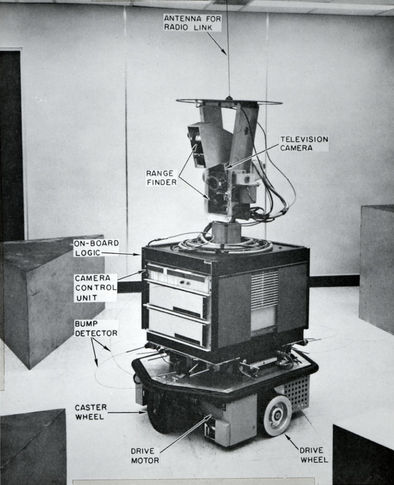
\includegraphics[height=8.0cm]{img/cap2/RobotShakey.jpg}}
\label{fig:RobotShakey}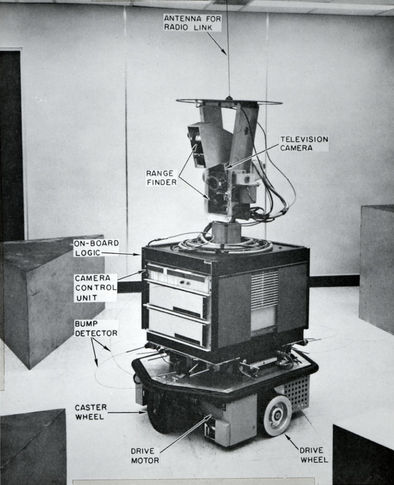
\includegraphics[height=8.0cm]{img/cap2/RobotShakey.jpg}
\end{center}
\caption{Robot Shakey. En los albores de la Visión Artificial}
\end{figure}


\subsection{Bloques habituales en sistemas de Visión Artificial}
La mayoría de sistemas de visión artificial o visión por computador están compuestos por dos elementos principales:  El sistema de adquisición de imágenes y el sistema de procesado de imágenes. El primero se compone de la iluminación, captura de imágenes y sistemas de adquisición de señales. El segundo implementa los algoritmos de visión que procesan las imágenes para extraer información de ellas.

	\textbf{- El sistema de iluminación}: Está compuesto por todos los elementos que iluminan los objetos con cualquier tipo de radiación electromagnética. Como ejemplo de estos artefactos podríamos citar la luz natural del sol, o la luz artificial proporcionada por lámparas, lasers o leds.

	\textbf{- El sistema de captura de imagen}: Transforma en señales eléctricas la luz que se refleja en los objetos. El elemento más utilizado son las cámaras, tanto de espectro visible como de espectro invisible.

	\textbf{- El sistema de adquisición de señales}: Las imágenes capturadas por las cámaras se utilizan para generar señales de vídeo. Su principal objetivo es enviar la señal de vídeo a la entrada de datos del ordenador.

	\textbf{- Sistema de procesamiento}: Suele ser un ordenador u otro dispositivo con capacidad de computación que implementa los algoritmos necesarios para procesar la imagen digital y para elaborar la información requerida por el sistema de visión artificial

	El sistema de procesamiento de imágenes suele componerse de las siguientes fases:
    \begin{enumerate}
		\item{Preproceso}: Durante esta fase la imagen puede ser adaptada para extraer mejor la información requerida por los algoritmos o métodos usados. El principal objetivo de esta fase es obtener una mejor calidad de la imagen de entrada, usando técnicas como filtrados de ruidos, convolución, resaltado de bordes etc.

		\item{Segmentación}: En esta fase la imagen es dividida en áreas de interés. Por ejemplo diferenciando objetos cuadrados de objetos esféricos o seleccionando las líneas de la carretera obviando el resto de la imagen. Para este propósito se pueden utilizar varias técnicas: umbrales, discontinuidades, crecimiento de regiones, filtros de color, detección de movimiento, etc

		\item{Clasificación}: Una vez la imagen ha sido dividida por regiones de interés (\textit{Regions of Interest}), se pueden extraer las características específicas de cada una. Esto puede realizarse por análisis morfológico , por texturas o usando técnicas de clasificación de color.
	\end{enumerate}

	\textbf{- Sistemas Periféricos}: Se trata de los elementos receptores de información, incluyendo monitores, dispositivos que usan la información par tomar decisiones etc.

\subsection{Aplicaciones de Visión Artificial}
Hoy en día, el número de aplicaciones de visión por computador está creciendo muy deprisa, debido a la disponibilidad de hardware barato que es capaz de ejecutar complejos algoritmos de visión artificial en un tiempo razonable. Por ejemplo, podemos encontrar aplicaciones en robótica para vehículos no tripulados, en medicina la visión artificial ya ayuda en diagnósticos mediante análisis de imágenes de los pacientes ( cáncer, enfermedades degenerativas, etc), en astronomía ayuda a generar imágenes de mayor calidad etc.

Actualmente, la visión artificial se utiliza en muchos procesos científicos, industriales y militares, por ejemplo para el reconocimiento de objetos o en el seguimiento de éstos:

	\textbf{Reconocimiento de objetos}: Se trata de buscar unas propiedades concretas de un determinado objeto (forma, color o cualquier otro patrón) en una imagen para determinar si un objeto se encuentra o no en ella. Por ejemplo mediante la obtención de píxeles característicos que destaquen en la imagen o utilizándose técnicas de \textit{Deep Learning} con redes neuronales.

	\textbf{Seguimiento de objetos}: Tras ser detectado, se pueden realizar tareas de seguimiento de un objeto. Podrá efectuarse dicho seguimiento teniendo en cuenta sus propiedades (texturas, bordes, etc) o analizando su desplazamiento respecto a imágenes anteriores.

	\textbf{Reconocimiento de caracteres (OCR)}:  Una de las aplicaciones más populares para la visión artificial es el reconocimiento de caracteres (OCR). El propósito de estos sistemas son la identificación de caracteres, por ejemplo hay aplicaciones que te permiten sacar una foto a la lista de componentes de un producto envasado y la aplicación gracias al OCR puede revisar todos los ingredientes del alimento y avisar si el producto contiene algún elemento al que pueda ser alérgico el usuario, como por ejemplo el gluten.

	\textbf{Aplicaciones de realidad aumentada}: gracias a la Visión Artificial es posible capturar imágenes del mundo real y procesarlas añadiendo la posibilidad de introducir en estas imágenes elementos artificiales nuevos (gráficos 3D) que encajarían en las dimensiones de las imágenes capturadas. Por ejemplo podríamos captar imágenes de una habitación de la casa a través de la cámara del móvil y mediante realidad aumentada añadir mobiliario nuevo virtual que sólo sería observable desde la pantalla del smartphone.

\begin{figure}[htbp]
\begin{center}
\label{fig:realiadAumentada}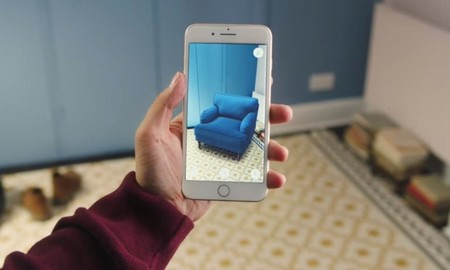
\includegraphics[height=8.0cm]{img/cap2/realidadAumentada.jpg}
\end{center}
\caption{Ejemplo de realidad aumentada, el sillón sólo existe en la pantalla del smartphone}
\end{figure}


\section{Visual SLAM}

\textit{Visual Simultaneous Localization And Mapping} (Localización y Mapeo Visual Simultaneo). Se refiere al proceso de estimar la posición y orientación de una cámara con respecto al mundo que le rodea, mientras que simultáneamente mapea el espacio que rodea a la cámara gracias a un procedimiento que analiza y extrae información de las imágenes capturadas por dicha cámara.

Visual SLAM es un tipo específico de sistema SLAM que se basa en algoritmos de visión 3D
para realizar tareas de autolocalización y mapeo cuando ni la localización de la posición de la cámara ni el entorno son conocidos.

La mayoría de los sistemas SLAM funcionan estimando la posición de un conjunto de puntos en varias imágenes sucesivas y así triangular la posición 3D, mientras que simultáneamente utiliza esta información para dar un posición aproximada de la cámara. Básicamente, el objetivo de estos sistemas es hacer un mapa de sus alrededores de su localización para así poder realizar tareas de navegación por el entorno.

Esto es posible con una sola cámara. Mientras existan un número suficiente de puntos que puedan ser seguidos a través de varios fotogramas, tanto la orientación del sensor de orientación como la estructura física del entorno pueden ser rápidamente estimados.

Todos los sistemas Visual SLAM están constantemente trabajando para minimizar el error de reproyección, o la diferencia entre los puntos reales y los puntos proyectados, para ello suele utilizar una solución llamada \textit{Bundle Adjustment}.




\subsection{Aplicaciones en Visual SLAM} 

Visual SLAM es todavía una tecnología emergente, pero con muchísimo potencial. Es una parte importante en aplicaciones de realidad aumentada, ya que esta tecnología es capaz de mapear el mundo físico con gran exactitud. También se utilizará en una gran variedad de robots, por ejemplo, los robots que se envían a Marte utilizan sistemas de Visual SLAM para navegar de forma autónoma. De la misma manera drones y robots en agricultura pueden utilizar esta misma tecnología para moverse por campos de cultivo, incluso los vehículos autónomos podrían utilizar sistemas Visual SLAM para mapear y entender el mundo a su alrededor. Otro gran potencial del Visual SLAM es que permite reemplazar el GPS en ciertos entornos, ya que el GPS no es muy útil en interiores y en grandes ciudades, donde el GPS tiene una exactitud de metros mientras que con Visual SLAM no existirían estos problemas y además tiene mayor exactitud.
A continuación se expondrán varios ejemplos de aplicaciones, desde teléfonos móviles hasta robots aspiradora.
\begin {enumerate}
%\subsection{Proyecto Tango}
\item \textbf{Proyecto Tango:}

El proyecto Tango es un proyecto colaborativo que trata de equipar a los smartphones y Tablets con sistema operativo Android la capacidad de medir la profundidad a la que se encuentra cada píxel de las imágenes capturadas por la cámara. Para ello los dispositivos compatibles con Tango dispondrán de 2 cámaras, una cámara RGB y otra que captura la profundidad, así el smartphone es capaz de construir un mapa en 3D del entorno (Figura \ref{fig:prototipoTango}). 
\begin{figure}[htbp]
\begin{center}
\subfigure[]{\label{fig:lenovo}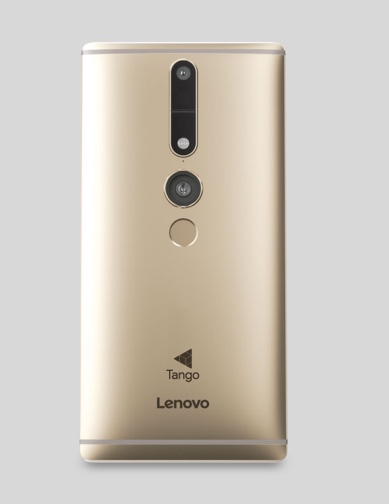
\includegraphics[height=4.5cm]{img/cap2/lenovo-phab2-pro.jpg}}
\hspace{0.5cm}
\subfigure[]{\label{fig:zenfone}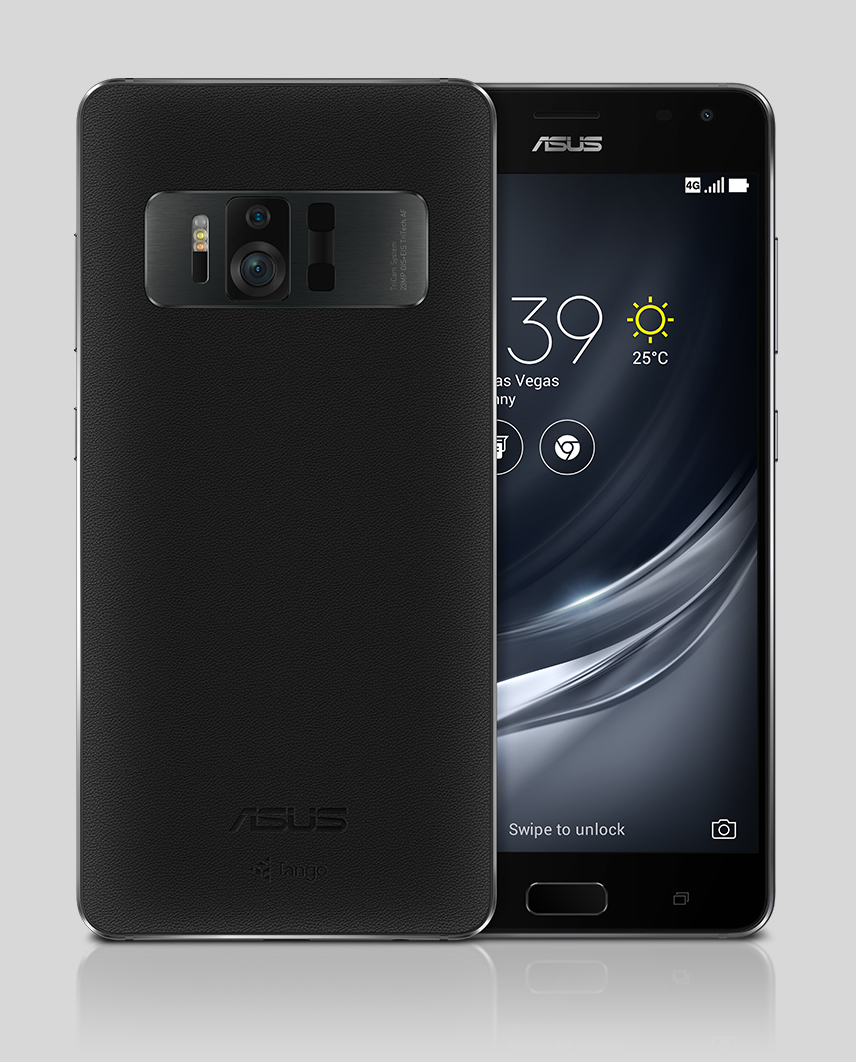
\includegraphics[height=4.5cm]{img/cap2/asus-zenfone-ar.jpg}}
\hspace{0.5cm}
\subfigure[]{\label{fig:prototipoTango}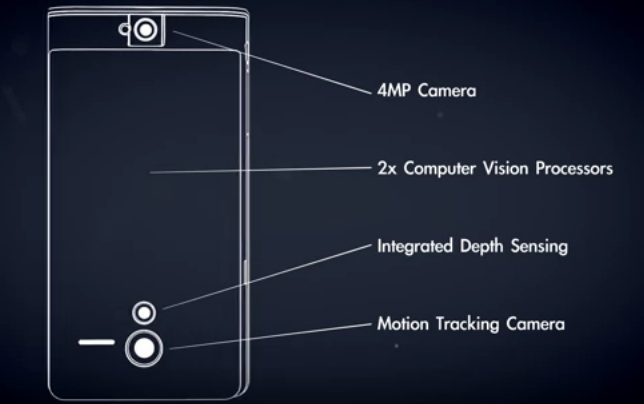
\includegraphics[height=4.5cm]{img/cap2/prototipo_Tango_smartPhone.png}}
\hspace{0.5cm}
\end{center}
\caption{El primer smartphone compatible con Tango de Lenovo(a). El primer Smartphone compatible con Tango y DayDream de ASUS (b).Esquema de prototipo de smartphone Tango (c).}
\end{figure}
Las posibilidades que ofrecerán este tipo de dispositivos serán muy variadas, desde medir las dimensiones de la habitación, hasta lo más útil como guiar a personas con discapacidades visuales en el interior de edificios. Pero también tendrá utilidades para el entretenimiento como convertir una habitación en el escenario de un juego mediante realidad aumentada.

Al ser una tecnología nueva aún no hay un elevado número de dispositivos que lo soporten. De momento existen 2 móviles compatibles con Tango \footnote{https://get.google.com/tango/}, el Lenovo  Phab 2 pro (Figura \ref{fig:lenovo}) y el Asus Zenfone AR (Figura \ref{fig:zenfone}).
En el caso del Zenfone AR  estará equipado con 3 cámaras traseras, una para seguir objetos (\textit{motion tracking}), otra para detectar profundidad y otra de alta resolución de 23 MP.
Con estas 3 cámaras el smartphone podrá crear una modelo tridimensional del entorno y seguir su movimiento. La cámara de localización permitirá al ZenFone conocer su posición 3D en todo momento mientras se mueve por el entorno. La cámara de profundidad está equipada con un proyector de Infrarrojos que le permite medir distancias hasta los objetos en el mundo real.

\begin{figure}[htbp]
\begin{center}
\subfigure[]{\label{fig:mapaTango}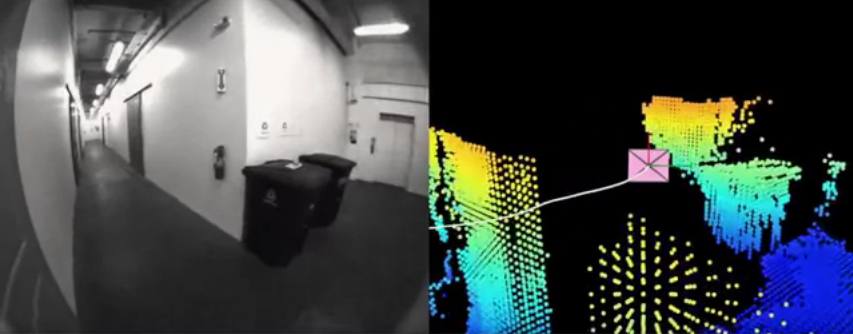
\includegraphics[height=3.0cm]{img/cap2/Proyecto_Tango_genera_mapa.png}}
\hspace{0.5cm}
\subfigure[]{\label{fig:makingMapTango}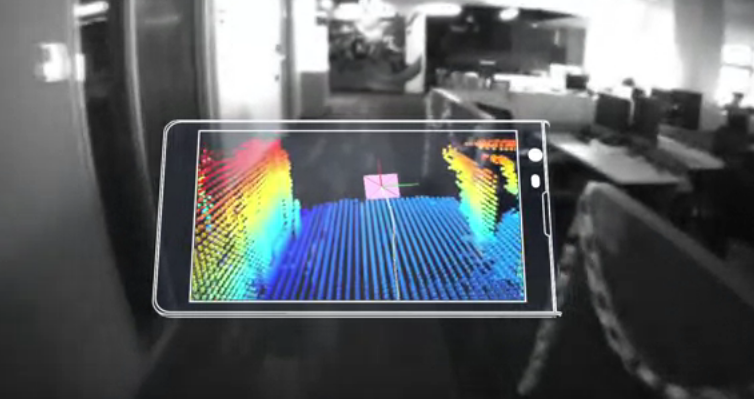
\includegraphics[height=3.0cm]{img/cap2/tangoDeviceMakingMap.png}}
\end{center}
\caption{Generación de mapa 1 (d). Generación de mapa 2 (e)}
\end{figure}

\clearpage

%\subsection{Magic Plan}
\item \textbf{Magic Plan:}

Magic Plan es una aplicación que permite de forma interactiva obtener planos de habitaciones o del interior de un edificio, utilizando para ello la cámara de nuestra tablet o smartphone, sólo es necesario sacar fotos. Esta aplicación es gratuita, aunque si se desea obtener el plano en formato digital (pdf, jpg, csv y otros) será necesario pagar una pequeña cantidad de dinero.
Es muy sencilla de utilizar y en cuestión de minutos se obtiene un plano fiable sin necesidad de medir, dibujar, mover muebles  y sin necesidad de ser un experto.
La aplicación utiliza técnicas de Visual SLAM y se apoya también en la información de los giroscopios de los dispositivos. Es compatible con Android y dispositivos Apple.

En el caso de Android, actualmente la última versión es compatible con el sistema Tango, por tanto el procedimiento de captura es mucho más sencillo, robusto y preciso  ya que  permite detectar con mayor exactitud todas las paredes de la habitación, visualizarlas en 3D y aplicar realidad aumentada.

%\begin{figure}[htbp]
%\begin{center}
%\subfigure[]{\label{fig:magicPlan}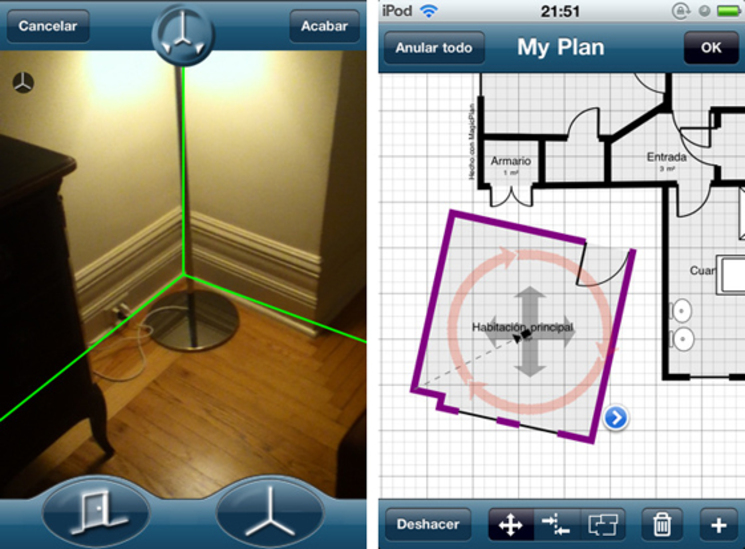
\includegraphics[height=8.0cm]{img/cap2/MagicPlan.jpg}}
%\end{center}
%\caption{La pantalla de un smartphone utilizando Magic Plan. }
%\end{figure}

%\clearpage

%\subsection{Pix4D}
\item \textbf{Pix4D:}

Pix4D \footnote{https://pix4d.com/} es un software especializado en fotogrametría. Permite la posibilidad de generar mapas 2D y 3D desde fotografías. Las imágenes pueden ser transmitidas vía wireless a Pix4DDim para procesarlas y convertirlas a mapas 2D y 3D.  Posteriormente esta información será accesible desde la nube para poder analizarlas y compartirlas.
Pix4D permite crear mapas con exactitud a partir de fotografías de interiores, también tiene aplicaciones en minería para medir superficies y volúmenes (Figura \ref{fig:volumen}) de minas a cielo abierto, incluso se utiliza con finalidades forenses para recrear en 3D escenarios de accidentes, que posteriormente pueden ser analizadas con todo detalle.
También tiene aplicaciones en la agricultura para obtener mapas de cosechas utilizando la información que proporcionan las cámaras especiales como la Parrot Sequoia (Figura \ref{fig:parrotSequoia}).
Con la aplicación Pix4DCapture podremos controlar un dron desde nuestro smartphone para que genere un mapa. El dron puede volar de forma autónoma siguiendo algunas de las trayectoria de vuelo que trae por defecto el producto o también puede generar el mapa mientras lo teledirigimos.

%\begin{figure}[htbp]
\begin{figure}[H]
\begin{center}
\subfigure[]{\label{fig:volumen}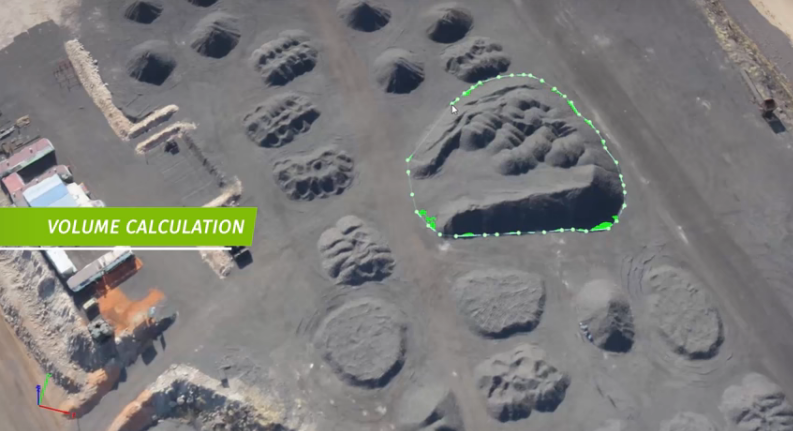
\includegraphics[height=3.0cm]{img/cap2/pix4d_volumen_calculo.png}}
%\hspace{0.5cm}
%\subfigure[]{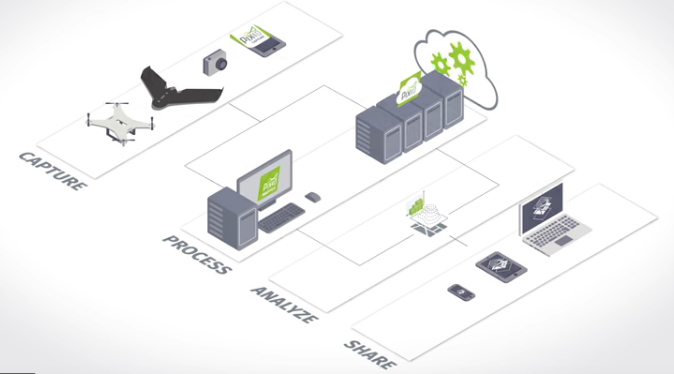
\includegraphics[height=3.0cm]{img/cap2/pix4d_esquema.png}}
%\hspace{0.5cm}
%\subfigure[]{\label{fig:dronTrayectoria}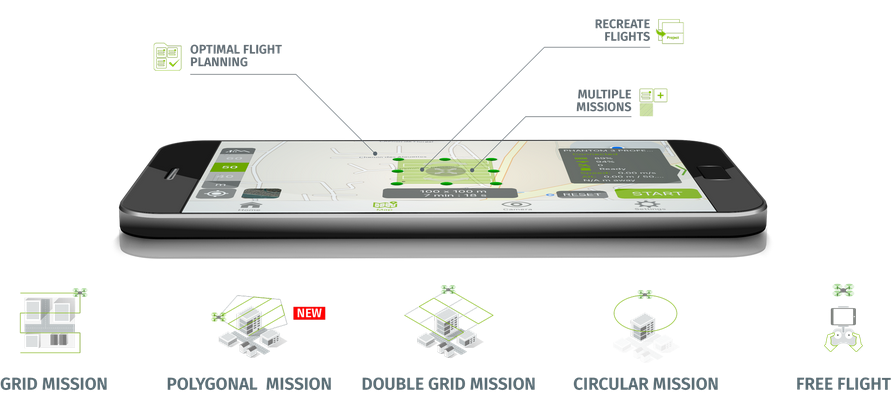
\includegraphics[height=4.0cm]{img/cap2/pix4d_dron_trayectorias.png}}
\hspace{0.5cm}
\subfigure[]{\label{fig:parrotSequoia}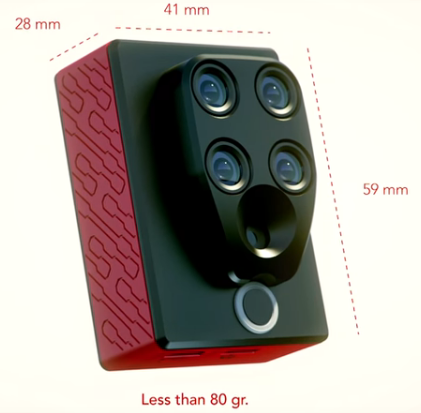
\includegraphics[height=4.0cm]{img/cap2/parrotSequoia.png}}
\end{center}
\caption{Pix4D cálculo de volumen(a). Cámara multiesprectral Parrot Sequoia (b)}
\end{figure}
%\clearpage

%\subsection{Photo Tourism}
\item \textbf{Photo Tourism:}

PhotoTourism o Photo Synth es un software inicialmente creado por la universidad de  Washington en colaboración con Microsoft. Es un sistema que toma grupos de conjuntos de fotografías disponibles online sobre un lugar en concreto, normalmente sobre un monumento turístico mundialmente conocido (como NotreDame, el Coliseo ( Figura \ref{fig:Coliseo}), La Fontana de Trevi) y es capaz de reconstruir puntos 3D de los monumentos y también calcular o estimar la posición de la cámara desde donde se tomaron las fotografías. Proporciona una nueva forma de navegar a través de fotografías de un destino turístico y una nueva forma de hacer visitas virtuales a monumentos.
Este sistema utiliza la técnica de \textit {Structure From Motion} SFM. SFM encuentra coincidencias de  puntos característicos entre distintas fotografías de un mismo lugar y que han sido tomadas desde distintos puntos de vista y así es capaz de calcular la localización 3D de dichos puntos característicos y también la localización 3D desde donde se tomaron las fotografías.
A diferencia de Visual SLAM, el procesamiento de estas fotografía es offline, sin necesidad de tiempo real, por lo que pueden ser ejecutadas desde un PC que por lo general tiene una capacidad de computación mucho mayor que una tablet o teléfono móvil.

\begin{figure}[htbp]
\begin{center}
\label{fig:Coliseo}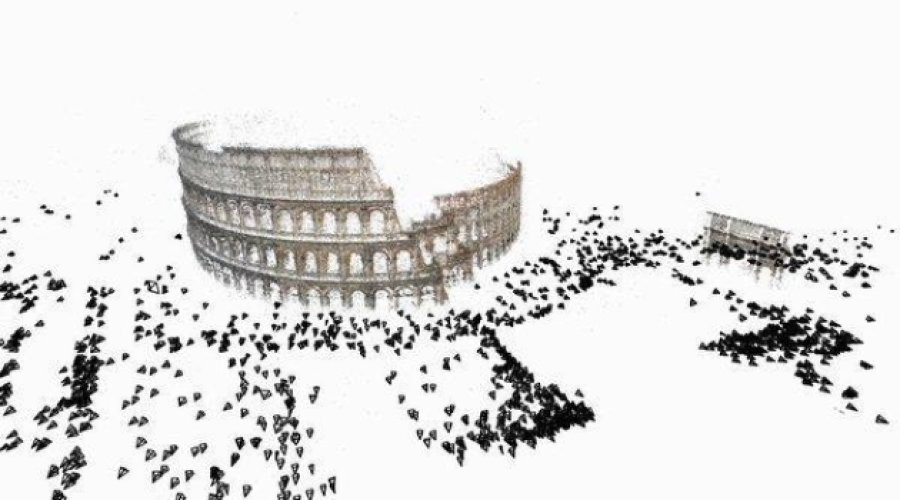
\includegraphics[height=8.0cm]{img/cap2/PhotoTourism.jpg}
\end{center}
\caption{Recreación del Coliseo de Roma generado con Photo Tourism. }
\end{figure}
%\clearpage

%\subsection{Canvas y el sensor Structure}


\item \textbf{Canvas y el sensor Structure:}

Canvas \footnote{https://canvas.io/ } es una herramienta de escaneo 3D enfocada a profesionales de la construcción o incluso aficionados al bricolaje en casa. La aplicación se ayuda del sensor de profundidad Structure. Este sensor se acopla en la parte trasera de un Ipad. Canvas permite obtener los planos en 3D de cualquier habitación de una manera fácil y sencilla, simplemente tendremos que pasear el Ipad equipado con el sensor Structure \footnote{https://structure.io/} alrededor de la habitación y podremos ver como el mapa 3D comienza a generarse en tiempo real. El sensor (Figura \ref{fig:Structure}) toma miles de medidas de profundidad que utilizará para generar el plano tridimensional. Los planos son almacenados en el Ipad y pueden ser consultados de manera interactiva posteriormente. Además permite que los planos generados sean convertidos a ficheros CAD.

\begin{figure}[htbp]
\begin{center}
\label{fig:Structure}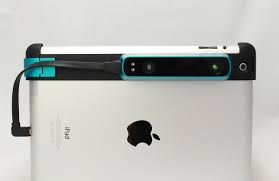
\includegraphics[height=5.0cm]{img/cap2/structureSensorCanvas.jpg}
\end{center}
\caption{El sensor de profundidad Structure para Ipad. }
\end{figure}

%\clearpage



\item \textbf{Robot Aspirador:}
Recientemente ha entrado en los hogares el uso de Visual SLAM gracias a los últimos modelos de aspiradora equipados con cámaras.
Estos aspiradores robotizados disponen de cámaras que le permiten obtener un mapa de la habitación o planta del edificio y gracias a este mapa son capaces de aspirar toda la superficie del suelo de la habitación de manera eficiente, sin dejar ninguna zona de la planta sin limpiar. Además están equipados con sensores de proximidad, que les permiten esquivar obstáculos y aunque tengan que modificar su recorrido momentáneamente son capaces de seguir limpiando ya que pueden utilizar el mapa para continuar su ruta. Entre los distintos aspiradores estarían:
Aspirador Dyson 360 Eye (Figura \ref{fig:Dyson})\footnote{http://www.dyson.come}, Aspirador Roomba 966 (Figura \ref{fig:roomba})\footnote{http://www.irobot.es/robots-domesticos/aspiracion}, Aspirador LG-Hombot \footnote{http://www.lg.com/es/aspiradoras/lg-VR64702LVMT}

Tanto el modelo de Dyson como Roomba utilizan una cámara de 360 grados, 
en cambio el modelo de LG utiliza una doble cámara, y es capaz de aspirar la casa incluso en la oscuridad.

%\begin{figure}[htbp]
\begin{figure}[H]
\begin{center}
\subfigure[]{\label{fig:Dyson}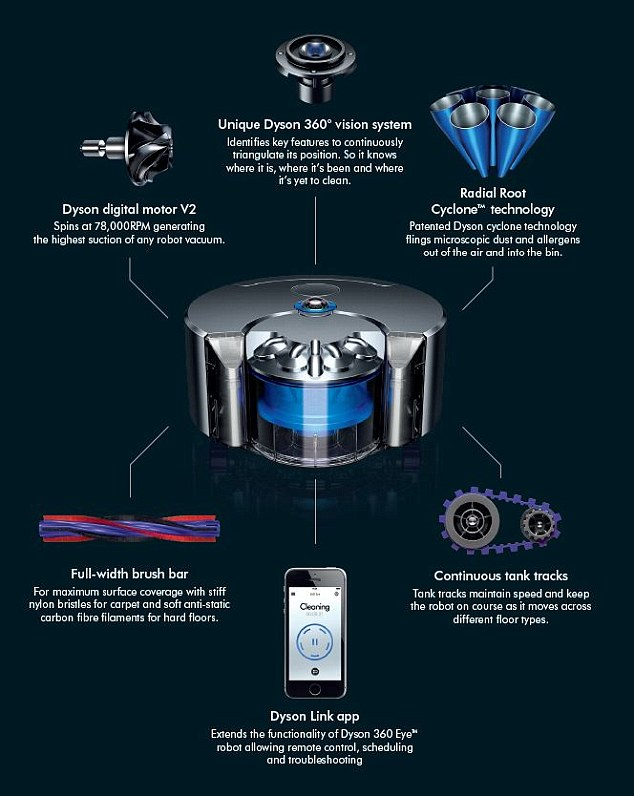
\includegraphics[height=6.0cm]{img/cap2/Dyson_360.jpg}}
\hspace{0.5cm}
\subfigure[]{\label{fig:roomba}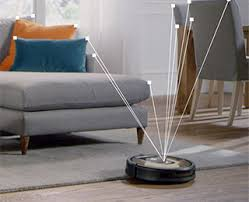
\includegraphics[height=6.0cm]{img/cap2/roomba_966.jpg}}
\hspace{0.5cm}
%\subfigure[]{\label{fig:LG_hombot}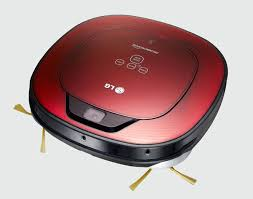
\includegraphics[height=6.0cm]{img/cap2/LG_hombot.jpg}}
\end{center}
%\caption{Robot Dyson 360 Eye (a) Robot Roomba 966 (b) Robot Hombot de LG (c).}
\caption{Robot Dyson 360 Eye (a) Robot Roomba 966 (b) }
\end{figure}

\item \textbf{Drones:}

Por último no podemos olvidar los drones, robots voladores equipados con cámara que también pueden obtener mapas de su entorno con Visual SLAM. Existen también proyectos para equipar a drones con dispositivos compatibles con Tango para que sean capaces de obtener mapas de interiores con mayor precisión, robustez y velocidad \footnote{http://spectrum.ieee.org/automaton/robotics/drones/autonomous-quadrotor-flight-based-on-google-project-tango}.


%\begin{figure}[htbp]
\begin{figure}[H]
\begin{center}
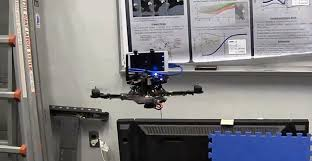
\includegraphics[height=5.0cm]{img/cap2/droneTango.jpg}
\end{center}
\caption{Dron equipado con dispositivo compatible con Tango}
\end{figure}

\end {enumerate}



\subsection{Conceptos}

Conviene explicar una serie de conceptos relacionados con Visual SLAM ya que aparecerán más adelante cuando expliquemos en profundidad los algoritmos más importantes que existen hoy en día para localización visual.

\textbf{Calidad}: La calidad del algoritmo de Visual SLAM dependerá de tres factores. La eficiencia temporal, la precisión espacial en la estimación de la posición y la robustez del algoritmo.

\textbf{Eficiencia}: Mediremos la eficiencia como el tiempo de ejecución de cada iteración del algoritmo. Los algoritmos deberán ser capaces de procesar al menos 30 fotogramas por segundo

\textbf{Precisión}:  El error lineal y error angular entre la posición estimada y la posición lineal determinará la precisión. Mediremos el error lineal como la distancia euclídea entre las dos posiciones, mientras que el error angular vendrá determinado por la diferencia entre las 2 orientaciones.

\textbf{Robustez}: Diremos que el algoritmo de localización es robusto siempre que pueda seguir funcionando con normalidad tras encontrarse con una situación imprevista (como una oclusión, secuestros, movimiento de objetos en la escena, mala calidad de imagen, etc)

\textbf{Oclusiones}: Cuando la cámara del robot esté tapada parcial o totalmente se producirá una oclusión, por tanto no se podrá extraer información en la región de la imagen ocluida. Los algoritmos deben estar preparados para cuando existan oclusiones.

\textbf{Secuestros}: Se producirá un secuestro cuando la cámara o robot sea movida deliberadamente por un tercero, de tal forma que los cálculos de la posición anterior ya no sean válidos. Los algoritmos deberían detectar secuestros e intentar localizarse desde su nueva posición.

\textbf{Localización Absoluta}: se produce cuando tenemos un mapa conocido, si estimamos la posición del robot dentro del mapa en coordenadas respecto del origen de coordenadas de ese mapa.

\textbf{Localización Incremental}:  En entornos con mapa desconocido, la localización del robot se establecerá de forma incremental respecto de posiciones previas pasadas ( por ejemplo en el instante anterior), lo que dará lugar a un error en la localización incremental que aumentará con el tiempo.

\textbf{Cierre de bucle}: Se produce cuando el robot vuelva a pasar por una zona del mundo que ya haya visitado anteriormente. Si se vuelve a pasar por el punto de origen se puede determinar el error que se ha producido comparando la posición real en el origen con la estimada por el algoritmo de localización.

\textbf{Relocalización}: Si tras un secuestro, el robot consigue recuperarse y estima correctamente la posición absoluta del robot dentro del mapa.


\subsection{Problemas abiertos en Visual SLAM} \label{s:problemavlsam}

Actualmente las técnicas de Visual SLAM presentan algunos problemas o inconvenientes que todavía son difíciles de sortear en la práctica. En esta sección presentaremos algunos de ellos:
\begin {enumerate}
\item \textbf{Inicialización del Mapa:}

Si en Visual SLAM queremos conseguir una estimación lo más exacta posible de la posición de la cámara es necesario contar con una buena inicialización del Mapa. Se debe contar con un sistema de coordenadas globales definido, y se tomarán puntos de referencia del entorno como puntos iniciales del mapa en el sistema global de coordenadas. Utilizando este método podemos inicializar Visual SLAM en un sistema de coordenadas global en la tierra. La transformación de estos puntos iniciales al sistema de referencia global se realizará mediante homografía.

Objetos de referencia como objetos 3D también se han utilizado para obtener un sistema global de coordenadas, posiciones iniciales de la cámara son estimadas gracias al seguimiento de objetos de referencia.
En Mono SLAM (cap 3,sec 1), por ejemplo, se utilizan al menos 4 puntos 3D (que se corresponden con las esquinas de un folio) como objetos de referencia.

\item \textbf{Ambigüedad en la escala:}

En algunas aplicaciones con Visual SLAM se necesita información de escala absoluta. Para obtener una referencia de escala absoluta se pueden utilizar zonas de la anatomía del usuario, como la cara, su mano o el propio cuerpo u otros objetos de tamaño conocido. En todos estos métodos se asume que entre personas la diferencia de tamaño es mínima para dichas partes del cuerpo. Se han dado otras aproximaciones como utilizar algunos de los sensores con los que ya están equipados la mayoría smartphones tales como acelerómetros, giroscopios y sensores magnéticos. Para eliminar el ruido de estos sensores se utiliza una técnica de filtro de dominio de frecuencia.


\item \textbf{Dificultad para operar en entornos con pocas texturas:}

Visual SLAM utiliza el emparejamiento de píxeles o puntos característicos entre varios \textit{frames} consecutivos. El emparejamiento suele fijarse en esquinas, bordes  o puntos distintivos que fácilmente podrán localizarse entre frames. Pero cuando en el entorno hay pocas texturas o presenta una alta monotonía de texturas,  el emparejamiento es difícil de realizar ya que un punto en un fotograma podría corresponder con N puntos en el siguiente fotograma y por tanto se dispararía el error de posición. Quizá este sea uno de los problemas más difíciles de solucionar con Visual SLAM
\cite{Takafumi17}.

\section{Estructura del documento}
El presente documento está dividido en 6 secciones y trata de describir este TFM, cuya temática  es la creación de una herramienta de evaluación de algoritmos de Visual SLAM. 
El primer capítulo es una introducción a la Visión Artificial y Visual SLAM, donde se explica en que consiste Visual SLAM, sus aplicaciones y cuales son las principales dificultades que debemos solventar a la hora de implementar un algoritmo de Visual SLAM. 
El capítulo 2 será una descripción detallada de los principales objetivos del TFM.
El capítulo 3 estará dedicado al Estado del Arte de los algoritmos Visual SLAM, y también se expondrán las herramientas más conocidas hoy en día para la evaluación de algoritmos Visual SLAM. 
En el capitulo 4 hablaremos de SLAMTestbed, una herramienta software creada precisamente en este TFM para evaluación de algoritmos Visual SLAM.
En el capítulo 5 se expondrán los distintos experimentos y tests realizados para evaluar la herramienta SLAMTestbed.
Y por último, el capitulo 6, donde se muestran las conclusiones del TFM.


\end {enumerate}
%\vfill
%\\raggedbottom 
%\parskip=1pt
%\vspace*{1in}
\flushbottom
\clearpage
\newpage
\pagebreak






\chapter{Objetivos} \label{cap:Objetivos}
%\section{Objetivos} \label{s:objeticos}
%\pagenumbering{arabic}
%\setcounter{page}{1}

%\setcounter{section}{2}

En el siguiente capítulo se detallarán las metas concretas que se pretenden alcanzar en este Trabajo Fin de Máster.

\section{Objetivos}
Desde el nacimiento de Visual SLAM, se están desarrollando algoritmos que permitan a los robots estimar su posición, o con una cámara localizar una imagen en tiempo real en 3D para aplicaciones de realidad aumentada. Estos algoritmos son complejos y están compuestos de múltiples etapas, a menudo un ligero cambio en alguna de estas etapas puede hacer que los resultados del algoritmo mejoren significativamente o por el contrario empeoren. Sería muy útil y conveniente contar con una herramienta que permitiese analizar o estimar la bondad de los nuevos algoritmos visual SLAM.

\textbf{El objetivo principal de este proyecto es presentar una herramienta que permitan comparar cuantitativamente el rendimiento de los algoritmos Visual SLAM y la calidad de sus estimaciones}.
Esta herramienta permitirá comparar el rendimiento de los diferentes algoritmos de Visual SLAM así como estudiar más fácilmente que modificaciones o mejoras se podrían aplicar en los algoritmos ya existentes.

En  este TFM nos hemos centrado en medir la exactitud de las estimaciones de posición sin tener en cuenta la generación de mapas, es decir se ha puesto toda la atención en comparar las mediciones de \textit{tracking} dejando el \textit{mapping} para futuros proyectos. 

Entenderemos que un algoritmo A es mejor que otro B cuando el algoritmo A sea capaz de estimar la posición con mayor exactitud que otro algoritmo B en el menor tiempo posible y de manera robusta. La herramienta a desarrollar medirá la precisión de las estimaciones de posición y la agilidad entendiéndose esta como el tiempo de proceso dedicado a realizar dichas estimaciones de posición. 

Típicamente esta herramienta permitirá comparar dos secuencias de posiciones 3D, la estimada por un algoritmo de Visual SLAM y la secuencia de posiciones verdaderas. La diferencia entre ambas mide el error del algoritmo SLAM a la hora de estimar correctamente las posiciones de la cámara.
Este objetivo principal lo hemos articulado en los siguientes subobjetivos:

\begin {enumerate}
\item \textbf{Conseguir un Registrador Espacial:} Este registrador espacial debe permitir registrar 2 secuencias de puntos 3D en el espacio, estimando rotación, traslación y escala para poder realizar el registro espacial entre las 2 nubes de puntos.


\item \textbf{Registrador Temporal:} Que permita sincronizar las 2 secuencias de puntos 3D. Para ello deberemos ajustar los 2 secuencias a la misma frecuencia de muestreo, (utilizaremos interpolación) y también calcular el offset temporal entre ambas. El offset temporal sería la diferencia de tiempo entre 2 secuencias. 

\item \textbf{La herramienta de medición se validará experimentalmente:} Para comprobar que funciona correctamente realizaremos experimentos donde comprobaremos el error estimado entre la verdad absoluta (groundtrouth) y una secuencia transformada de la que se conoce exactamente el registro temporal y espacial. Se creará un Módulo de Transformación que permitirá realizar tanto alteraciones temporales como espaciales a una secuencia dada generando como resultado una nueva secuencia transformada.

\end {enumerate}

\section {Requisitos}

La solución que se desarrolle para alcanzar los objetivos deberá satisfacer además estos requisitos:


	\textbf{R1}. La herramienta debe restringirse a la comparación de algoritmos Visual SLAM que utilizan como sensor de visión una cámara RGB. Así quedan descartados los algoritmos que emplean cámaras RGBD.

	\textbf{R2}. Se restringirá solo a los algoritmos Visual SLAM que empleen \textit{una sola} cámara.

	\textbf{R3}. La herramienta debe ser aplicable a nuevos algoritmos de Visual SLAM.

	\textbf{R4}. Facilidad de uso.

	\textbf{R5}. Debe ofrecer una única métrica cuantitativa para la comparación entre varios algoritmos de Visual SLAM.

	\textbf{R6}. Debe ofrecer resultados fácilmente legibles y reconocibles para el usuario.

	\textbf{R7}. El software generado debe ser abierto y estar públicamente disponible.

\section{Metodología y plan de trabajo}

En cuanto a la metodología utilizada para desarrollar este TFM, se ha seguido el modelo de ciclo de vida en espiral. Una de las primeras lecciones que se aprenden de las metodologías ágiles es que la metodología debe adaptarse al proyecto y no al revés. Dicha premisa cobra más importancia en un proyecto realizado por una sola persona.

\begin{figure}[H]
\begin{center}
\subfigure[]{\label{fig:espiral}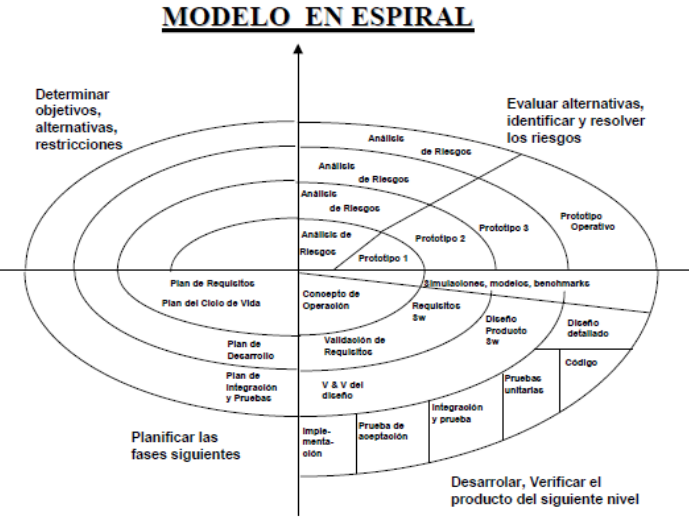
\includegraphics[height=6.0cm]{img/cap2/modeloEspiral.png}}
\end{center}
\caption{Inicialización de Mono SLAM con 4 puntos conocidos.}
\end{figure}


El modelo en espiral es un modelo iterativo, donde cada ciclo viene a representar una fase del proyecto software. Podemos diferenciar 4 fases dentro de cada ciclo del modelo en espiral

\textbf{-Determinar los Objetivos:} Determinaremos que metas se deben conseguir en cada iteración, teniendo en cuenta los objetivos del proyecto.

\textbf{-Evaluación de alternativas:} Evaluar las distintas alternativas para alcanzar las metas que se han establecido en la fase anterior, utilizando distintos puntos de vista.

\textbf{-Desarrollo y Evaluación:} Una vez seleccionada la mejor alternativa, se diseña y desarrolla el producto y por último se realizarán pruebas para testear su funcionamiento.

\textbf{-Planificación:} Teniendo en cuenta los resultados de las pruebas realizadas, se planificará la siguiente iteración revisando posibles errores cometidos en iteraciones anteriores y se comienza con una nuevo ciclo en espiral.

Por consiguiente, y enmarcándolo dentro de la metodología en espiral, primero se ha realizado un estudio previo muy amplio que sirve para obtener una visión completa del problema de Visual SLAM y detectar puntos críticos. Segundo se ha ido acotando hasta el primer prototipo del desarrollo principal, el cual ha sido revisado y validado en varias iteraciones. Este prototipo inicial es importante ya que no sólo nos permite avanzar en todas las vías en paralelo, sino porque ofrece una prueba de concepto para las ramificaciones que se han paralizado en favor del desarrollo troncal.

El proceso de desarrollo ha sido supervisado por los tutores mediante tres herramientas: reuniones semanales, definición de hitos y diario de trabajo.
Durante las reuniones se debían definir varios hitos de corto o medio plazo en los que se trabajaría esa semana. Este progreso se puede ver en la página web habilitada para tal uso:
\footnote{https://jderobot.org/Elias-tfm}

Así mismo, el código fuente desarrollado puede encontrarse en \footnote{https://github.com/JdeRobot/slam-Testbed} y la memoria en \footnote{https://github.com/RoboticsURJC-students/2017-tfm-elias-barcia}

\clearpage
\newpage
\pagebreak



%%\chapter{Problemas de Visual SLAM} \label{cap:problemavlsam}
\section{Problemas de Visual SLAM} \label{s:problemavlsam}

Actualmente las técnicas de Visual SLAM presentan algunos problemas o inconvenientes que todavía son difíciles de sortear en la práctica. En esta sección presentaremos algunos de ellos:

\subsection{Inicialización del Mapa:}

Si en Visual SLAM queremos conseguir una estimación lo más exacta posible de la posición de la cámara es necesario contar con una buena inicialización del Mapa. Se debe contar con un sistema de coordenadas globales definido, y se tomarań puntos de referencia del entorno como puntos iniciales del mapa en el sistema global de coordenadas. Utilizando este método podemos inicializar VisualSLAM en un sistema de coordenadas global en la tierra. La transformación de estos puntos iniciales al sistema de referencia global se realizará mediante homografía.

Objetos de referencia como objetos 3D también se han utilizado para obtener un sistema global de coordenadas, posiciones iniciales de la cámara son estimadas gracias al seguimiento de objetos de referencia.
En MonoSLAM por ejemplo se utilizan al menos 4 puntos 3D como objetos de referencia, y la forma del objeto se usa para mejorar el mapa.

\subsection{Ambigüedad en la escala:}

En algunas aplicaciones con Visual SLAM se necesita información de escala absoluta. Para obtener una referencia de escala absoluta se pueden utilizar zonas de la anatomía del usuario, como la cara, su mano o el propio cuerpo. En todos estos métodos se asume que entre personas la diferencia de tamaño es mínima para dichas partes del cuerpo. Se han dado otras aproximaciones como utilizar algunos de los sensores con los que ya están equipados la mayoría smartphones tales como acelerómetros, giroscopios y sensores magnéticos. Para eliminar el ruido de estos sensores se utiliza una técnica de filtro de dominio de frecuencia.

\subsection{Distorsión Rolling Shutter:}

Para conseguir una estimación de la posición de la cámara exacta, es importante considerar el tipo de shutter en la captura de la imagen. La mayoría de las técnicas de VisualSLAM asumen algoritmos \textit {global shutter}, y estos algoritmos estiman una posición de cámara para cada frame. Sin embargo existen en el mercado multitud de cámaras incluidas las RGB-D que emplean \textit {Rolling Shutter} debido a su coste. En las cámaras que utilizan el modo \textit{Rolling Shutter}, cada fila de una imagen capturada es tomada por una posición diferente de la cámara. Es obvio que es bastante complicado estimar directamente la posición de la cámara para cada fila. Se utilizará una aproximación basada en interpolación para estimar el \textit{Rolling shutter}. En algunas ocasiones se ha utilizado con éxito una función spline para interpolar la trayectoria de la cámara \footnote{https://www.premiumbeat.com/blog/know-the-basics-of-global-shutter-vs-rolling-shutter/}.

\begin{figure}[htbp]
\begin{center}
\subfigure[]{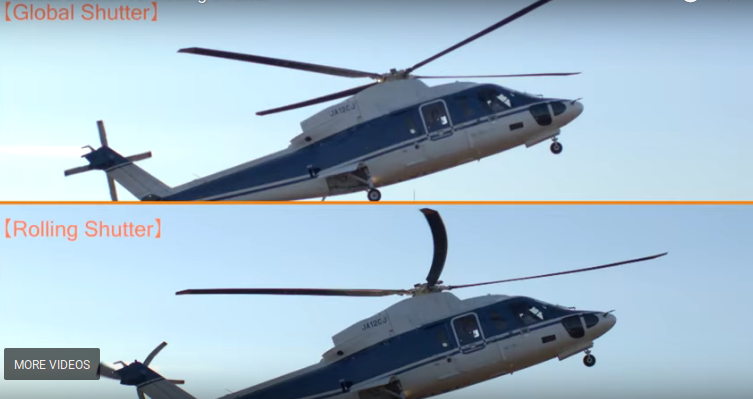
\includegraphics[height=5.0cm]{img/cap3/RollingShutter.png}}
\end{center}
\caption{Diferencias entre Global Shutter y Rolling Shutter (a)}
\end{figure}


\subsection{Dificultad para operar en entornos con pocas texturas:}

Visual SLAM utiliza el emparejamiento de píxeles o puntos característicos entre varios frames consecutivos. El emparejamiento suele fijarse en esquinas, bordes  o puntos distintivos que fácilmente podrán localizarse entre frames. Pero cuando en el entorno hay pocas texturas o presenta una alta monotonía de texturas,  el emparejamiento es difícil de realizar ya que un punto en un fotograma podría corresponder con N puntos en el siguiente fotograma y por tanto se dispararía el error de posición. Quizá este sea uno de los problemas más difíciles de solucionar con VisualSLAM
\cite{Takafumi17}.


\chapter{Estado del Arte} \label{cap:Estado del Arte}
%\section{Estado del Arte} \label{s:estado}

En esta sección explicaremos varios de los algoritmos SLAM más significativos , como MonoSLAM, PTAM, DTAM, SVO,LSD-SLAM,ORB-SLAM,DSO,SDVL y RGBD SLAM.
Tambien se describirán brevemente las distintas herramientas que existen en la actualidad para comparar las estimaciones de los algoritmos SLAM , comenzaremos por TUM, seguido de rgb trayectory evaluation , también describiremos la herramienta SLAMBENCH y por último daremos algunos detalles sobre The Kitti Vision Benchmark Suite.


\section{MonoSLAM}
El algoritmo de  MonoSLAM (\textit{Monocular SLAM}) \cite{Davison2007monoslam} utiliza solamente una cámara RGB para la localización y mapeo de entornos desconocidos. Fue desarrollado en el año 2002  por Andrew Robinson. Para estimar la posición de la cámara utiliza un filtro extendido de Kalman (EKF) y la posición de una serie de puntos 3D. Este método requiere de una inicialización con al menos 4 puntos 3D conocidos que utilizará para calcular la posición de la cámara y la generación de nuevos puntos para el mapa.
%\begin{figure}[htbp]
\begin{figure}[H]
\begin{center}
\subfigure[]{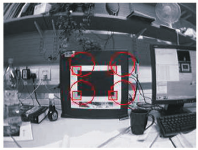
\includegraphics[height=6.0cm]{img/cap4/Initialization4PointsMonoSlam.png}}
\end{center}
\caption{Inicialización de MonoSLAM con 4 puntos conocidos.}
\end{figure}

El EKF, tiene un vector de estado compuesto de posición, orientación y velocidad de la cámara y además las coordenadas 3D de los puntos conocidos en un cierto momento, esto implica que el vector de estado irá aumentando de tamaño a medida que vayamos descubriendo nuevos puntos 3D. El modelo de observación estará compuesto de las proyecciones de cada uno de los puntos 3D en el plano imagen.

El uso de un EKF es apropiado, ya que se realizan iteraciones cada pocos milisegundos, y por tanto en intervalos de tiempo tan pequeños, el sistema puede aproximarse a un sistema lineal. Cuantas más iteraciones o frecuencia de muestreo la estimación mejora. En cada iteración se hace una detección de puntos de interés (esquinas con FAST) en la imagen actual de entrada, y obtendremos una serie de puntos que serán candidatos a ser el vector observación de los puntos que queremos seguir. Estos candidatos deberán ser filtrados, pues alguno puede ser un falsa esquina. Se utilizará una función de divergencia ZMSSD (\textit{Zero Mean Sum of Squared Differences}) entre parches para determinar si el candidato es aceptable o no. Al utilizar sólo parches de unos pocos píxeles alrededor del candidato, estamos optimizando el computo ya que no requiere procesar toda la imagen.

Aún así es posible que se acepten puntos candidatos que no sean apropiados. Para tratar de eliminar estos falsos positivos, \cite{civera20101} propuso una alternativa conocida como 1-Point RANSAC.
MonoSLAM es recomendable para mapas con pocos puntos. Es muy sensible a movimientos bruscos y por tanto difícilmente podrá recuperarse de un secuestro. Si la hipótesis de partida no es correcta el filtro podría desestabilizarse y no llegar nunca a aproximar razonablemente el vector de estado.


%\begin{figure}[htbp]
\begin{figure}[H]
\begin{center}
\subfigure[]{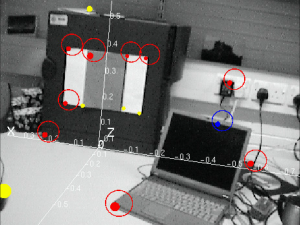
\includegraphics[height=5.0cm]{img/cap4/monoslam-300x225.png}}
\end{center}
\caption{Ejemplo de puntos característicos tomados con MonoSLAM.}
\end{figure}
\clearpage


\section{PTAM}
\textit{Parallel Tracking and \textit{Mapping}}. Es un algoritmo creado en 2007 por George Klein \cite{Klein2007parallel} que también calcula el Tracking y el \textit{Mapping} como en MonoSLAM pero para ello utiliza 2 \textit{Threads}, uno para calcular el posicionamiento de la cámara (Tracking ) y el segundo para la generación del mapa (\textit{Mapping}). Esta separación en dos hilos de ejecución se debe a que el Tracking necesita ser calculado en tiempo real para obtener una localización precisa, mientras que el \textit{Mapping} puede demorarse más tiempo sin perjudicar a la localización de la cámara. 

Con las imágenes captadas en secuencia se van generando \textit{Keyframes} o fotogramas clave. Se genera un nuevo \textit{Keyframe} a medida que la cámara se va desplazando. Los \textit{Keyframes} se utilizan para la localización y para ir generando el mapa de puntos.
Este algoritmo es recomendable para mapas con elevado número de puntos, es capaz de recuperarse fácilmente de un secuestro, extrae los puntos de interés mediante extracción de características como en MonoSLAM y trata de emparejarlos con los puntos extraídos de las imágenes anteriores.  Como extractor de características utiliza el detector FAST. Se realizará una subdivisión de la imagen a distintas resoluciones, normalmente 4 niveles, lo que se conoce como pirámide de la imagen y se pasará un filtro FAST sobre esta pirámide para detectar los puntos más característicos de la imagen.
Cada \textit{Keyframe} que se genera, contiene  la imagen captada junto su pirámide y sus puntos de interés detectados. Cuando añadimos un \textit{Keyframe}, se intenta localizar en este \textit{Keyframe} los puntos que ya se encuentran en el mapa, en caso de no ĺlocalizarlos se añaden nuevos puntos al mapa. Mientras no se añadan \textit{Keyframes}, se intentará mejorar el mapa con los \textit{Keyframes} disponibles optimizando con Bundle Adjustment.

Se suele utilizar en entornos cerrados y pequeños y utiliza técnicas SFM. Muy utilizado también para realidad aumentada.

%\begin{figure}[htbp]
\begin{figure}[H]
\begin{center}
\subfigure[]{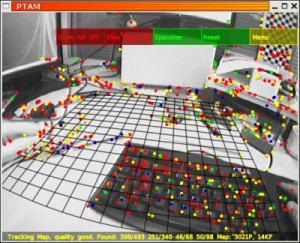
\includegraphics[height=6.0cm]{img/cap4/ptam_screenshot-300x243.jpg}}
\end{center}
\caption{Nube de puntos característicos tomados con PTAM.}
\end{figure}



\clearpage

\section{ORB-SLAM}
Es un algoritmo basado en extracción y emparejamiento de píxeles característicos mediante descriptores ORB, estos descriptores son más fiables que los parches tradicionales y por tanto permiten obtener mapas robustos y precisos tanto en escenarios de grandes dimensiones como en zonas pequeñas, sin embargo para su funcionamiento en tiempo real requiere la utilización de ordenadores con alta capacidad de proceso \cite{Mur2015orb}.
Puede ser utilizado con una cámara o dos e incluso con cámaras de profundidad RGBD. Para cierres de bucle y relocalización utiliza un modelo de bolsa de palabras \cite{galvez2012bags}.
Utiliza 3 \textit{Threads}, el primero para Tracking, el segundo para \textit{Mapping} y un tercero para detectar cierres de bucle. 

En el proceso de Tracking, se trata de calcular la posición actual a partir de los emparejamientos encontrados de los puntos 3D en el fotograma anterior, para ello utilizará los descriptores ORB.
En caso de perdida, el robot podrá relocalizarse gracias a un modelo de bolsa de palabras que le permitirá encontrar \textit{Keyframes} candidatos que concuerden con la observación actual (Figura \ref{fig:ORBMatching}).

En el proceso de \textit{Mapping}, se inicializarán 2 mapas, uno por homografía y el segundo mediante una matriz fundamental. Los 2 mapas recibirán una puntuación y se elegirá como candidato para inicializar el mapa aquel que obtenga mayor puntuación. Cuando ya se dispone del mapa inicial, se procesan los \textit{Keyframes} creando nuevos puntos 3D y se optimiza localmente el mapa mediante Bundle Adjustment. A su vez se genera un grafo donde cada \textit{Keyframe} se corresponde con un vértice y un vértice estará unido a otro siempre y cuando los \textit{Keyframe} tengan varios puntos 3D en común. Este grafo permite la eliminación de \textit{Keyframe} redundantes (Figura \ref{fig:ORB_SLAM}).

En el proceso de Looping, se comprobará si se ha producido un cierre de bucle. Utilizando el grafo de \textit{Keyframe} conectados y el modelo de bolsa de palabras se intenta encontrar \textit{Keyframe} candidatos que tengan una apariencia similar a la imagen actual.

%\begin{figure}[htbp]
\begin{figure}[H]
\begin{center}
\subfigure[]{\label{fig:ORBMatching}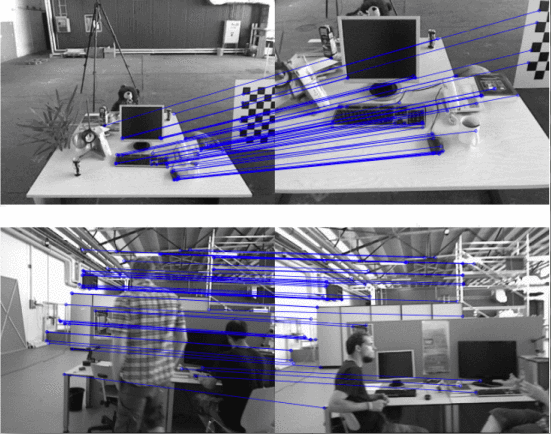
\includegraphics[height=5.5cm]{img/cap4/ORB_localization.png}}
\hspace{0.5cm}
\subfigure[]{\label{fig:ORB_SLAM}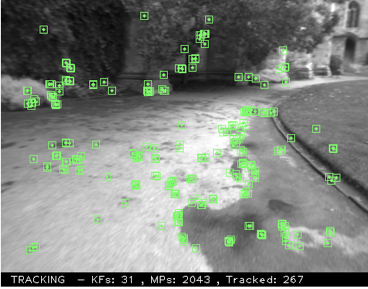
\includegraphics[height=5.5cm]{img/cap4/ORB_SLAM.png}}
\end{center}
\caption{Localización de puntos característicos en 2 imágenes con ORB }
\end{figure}

\clearpage

\section{DSO}
\textit{Direct Sparse Model}.
Está basado en optimizaciones continuas del error fotométrico sobre una ventana de frames recientes\cite{Engel2016direct}.
El inicio del Tracking, cuando se crea un nuevo \textit{Keyframe}, todos los puntos activos son proyectados en el y ligeramente dilatados, creando así un mapa de profundidad semi denso. Nuevos frames son creados con respecto a este frame utilizando alineamiento directo de 2 frames, una pirámide multi escala y un modelo de movimiento constante a inicializar. 
Para la relocalización, se podrán trazar hasta 27 rotaciones pequeñas en diferentes direcciones. Esta recuperación de posición se consigue en el nivel más pequeño de la pirámide de la imagen.
La creación de \textit{Keyframes} es similar a ORB-SLAM, existen 3 criterios para determinar cuando se necesita un nuevo \textit{Keyframe}.
\begin {enumerate}
\item Se creará un nuevo \textit{Keyframe} (Figura \ref{fig:mapaDSO}) cuando la imagen de entrada cambie notablemente con respecto al último \textit{Keyframe}, esto se medirá con la diferencias de medias al cuadrado entre los píxeles.
\item La traslación de la cámara causa oclusiones y des-oclusiones, lo cual indica que se deben generar nuevos \textit{Keyframes}
\item Si el tiempo de exposición de la cámara cambia significativamente, se deberá tomar un nuevo \textit{Keyframe}. Esto se mide por el factor de brillo relativo entre 2 frames. 
\end {enumerate}

En cuanto al rechazo de \textit{Keyframes}, sigue la siguiente estrategia. Sean $I_1$ \dots $I_n$ un conjunto de \textit{Keyframes} activos, siendo $I_1$ el más nuevo y $I_n$ el más antiguo
\begin {enumerate}
\item Siempre se mantendrán los dos últimos \textit{Keyframes} ($I_1$  e $I_2$ )
\item Frames con menos del 5\% de sus puntos visibles en $I_1$  son descartados.
\item Si mas de N frames están activos, se descartan (exceptuando $I_1$  e $I_2$) aquel que maximice un marcador de distancia d(i,j) donde d(i,j) es la distancia Euclídea entre \textit{Keyframes} $I_1$  e $I_j$
\end {enumerate}

Sobre el tratamiento de los puntos, siempre se tratará de mantener un numero fijo de puntos activos repartidos de forma uniforme entre el espacio y los frames activos. En un primer paso, se identifican Np puntos candidatos en cada nuevo \textit{Keyframe}. Los puntos candidatos no son inmediatamente sumados a la optimización, sino que son localizados individualmente en sucesivos frames generando una primera estimación del valor de profundidad que servirá como inicialización. 

En cuanto a la selección de puntos candidatos, se intentará seleccionar aquellos puntos que están bien distribuidos en la imagen y tienen un valor elevado de gradiente con respecto a sus alrededores. Para obtener una distribución uniforme de puntos sobre la imagen, esta se divide en bloques de $dxd$, de cada bloque se elegirá el píxel con el mayor gradiente siempre y cuando supere un umbral, de lo contrario no se selecciona el píxel de ese bloque. Los puntos candidatos son localizados en siguientes frames utilizando una búsqueda sobre la línea epipolar minimizando el error fotométrico. Una vez hallamos encontrado las coincidencias preparamos un valor de profundidad y la varianza asociada que se utilizará para restringir el intervalo de búsqueda en frames siguientes. Esta estrategia de localización está inspirada en LSD-SLAM.

Por último, la activación de puntos candidatos, cuando un conjunto de puntos antiguos son marginados, nuevos puntos candidatos son activados para remplazarlos, siempre intentando mantener una distribución uniforme de puntos por toda la imagen \footnote{https://ieeexplore.ieee.org/stamp/stamp.jsp?arnumber=7898369}.

%\begin{figure}[htbp]
\begin{figure}[H]
\begin{center}
\subfigure[]{\label{fig:mapaDSO}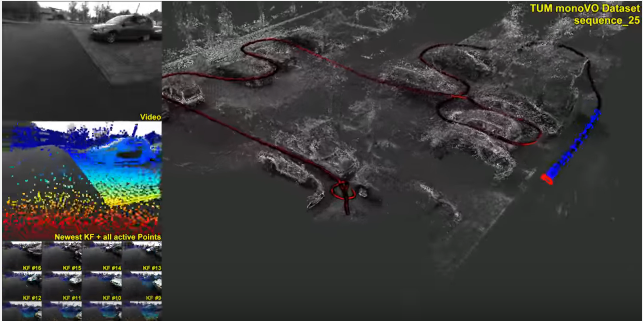
\includegraphics[height=6.0cm]{img/cap4/mapaDSO.png}}
\hspace{0.5cm}
\subfigure[]{\label{fig:fotogramaDSO}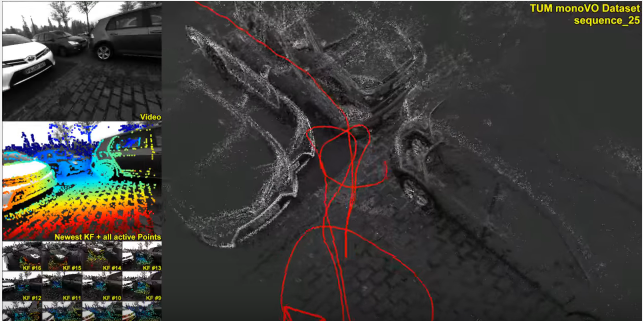
\includegraphics[height=6.0cm]{img/cap4/fotogramaDSO.png}}
\end{center}
\caption{Mapa generado con DSO (a) Ligero error en la posición al volver al punto de partida (b).}
\end{figure}

\clearpage

\section{LDSO}
\textit{LDSO: Direct Sparse Odometry with Loop Closure}. Este método es una extensión del algoritmo DSO (Direct Sparse Odometry). LDSO incorpora detección de cierre de bucle y optimización de posición y mapeo. Al ser un método directo, DSO puede utilizar cualquier pixel de la imagen con suficiente gradiente de intensidad, lo cual lo hace más robusto incluso en áreas donde apenas se pueden obtener puntos característicos. LDSO mantiene esta robusted, mientras que al mismo tiempo asegura la repetibilidad  sobre alguno de esos puntos prestando más atención sobre esquinas características en el proceso de tracking. Estas repetibilidad de puntos característicos permite detectar de forma fiable los candidatos de cierres de bucle utilizando la técnica basada en carácterísticas de bag-of-words. 
Los candidatos a cierre de bucle son verificados geométricamente y restricciones de pose relativa son estimadas minizando en conjunto errores geométricos 2D y 3D.
Selección de puntos de características Repetibles, DSO utiliza un grid dinamico para detectar suficientes pixels incluso en entornos con pocas texturas. Más especificamente, todavía se toma un numero determinado de pixeles ( por defecto 2000 en DSO), de los cuales algunos son esquinas. Manteniendo el número de esquinas pequeño se calculan los descriptores ORB y los empaquetamos en BoW. El algoritmo  utiliza ambos tipos de pixeles de esquinas y no esquinas para obtener el tracking, y la carga del thread para obtener el cierre de bucle permanece al mínimo.
En un frame capturado mediante DSO hay pocos elementos repetibles y por tanto es dificil buscar emparejamiento de imágenes usando esos puntos para cierre bucle. Pero en LDSO se utilizan ambos esquinas y otros pixeles con alto gradiente, donde las esquinas se utilizan para construir modelos BoW (Bag of Words) y para tracking, mientras que los no esquinas sólo se utilizan para tracking. De esta forma podemos hallar la posición en entornos con pocas texturas y tambien encontrar caracteristicas comunes entre keyframes si lo necesitasemos.
Cada vez que calculamos descriptores ORB para cada keyframe, una base de datos BoW es construida. Los candidatos a cierre de bucle son propuestos para el keyframe actual mediante consultas a la base de datos y solo se toman aquellos que están fuera de la actual ventana. Para cada candidato intentamos machear sus características ORB a aquellos del keyframe actual, y entonces ejecutamos RANSAC PnP para computarla estimación inicial de la transformación. Despues se optimiza la transformación usando el método de Gauss-Newton mediante la minimización de restricciones geométricas 3D y 2D.
\begin{figure}[H]
\begin{center}
\subfigure[]{\label{fig:LDSO}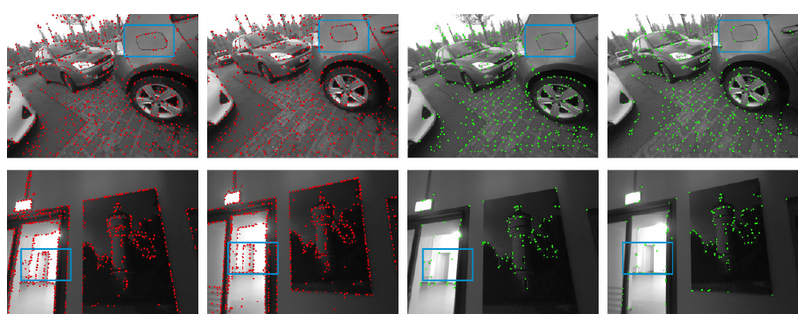
\includegraphics[height=6.0cm]{img/cap4/LDSO.png}}
\end{center}
\caption{diferencias entre puntos escogidos con DSO y LDSO.}
\end{figure}


\section{Herramientas para realizar evaluaciones comparativas de algoritmos SLAM}
En este apartado trataremos sobre varias herramientas que podemos utilizar para hacer benchmarking sobre los resultados de algoritmos SLAM y evaluar y comparar dichos resultados

\begin {enumerate}
%\subsection{Computer Vision Group TUM}
\item\textbf{Computer Vision Group TUM}

Proporciona varias herramientas para evaluar el rendimiento de algoritmos VSLAM, permite evaluar trayectorias y compararlas con la trayectoria ground truth.\cite{sturm12iros}
Utiliza principalmente 2 métodos, el error absoluto de la trayectoria \textit{absolute trajectory error (ATE)} y el error relativo a la posición \textit{relative pose error (RPE)}. Podemos encontrar en la web HERE scripts descargables para ambas métricas.

Las trayectorias que vayan a ser evaluadas deben ser almacenadas en un archivo de texto, donde cada línea contendrá una única posición con el siguiente formato( 'timestamp tx ty tz qx qy qz qw')

Donde el campo timestamp, tipo float proporciona el número de segundos , tx ty tz que son de tipo float, dan la posición del centro óptico de la cámara con respecto al origen de coordenadas del mundo real , qx qy qz qw , también de tipo float, dan la orientación del centro óptico de la cámara  con respecto al origen de coordenadas del mundo real pero en formato de quaternio unidad.


%\begin {enumerate}
%\item \textbf{Absolute Trajectory Error (ATE)}
 \textbf{\textit{Absolute Trajectory Error (ATE)}}:
 El error absoluto de trayectoria mide la diferencia que existe entre cada punto de la trayectoria estimada y la trayectoria real. Como paso de preproceso se realiza una asociación entre la posición estimada con la posición ground truth utilizando el emparejamiento por timestamps o marcas de tiempo. Tras esta asociación, se alinea la trayectoria real con la estimada usando SVD (Singular Value Decomposition). Por último, el ordenador calula la diferencia entre cada par de posiciones y devuelve valores estadísticos como la media,mediana y desviación estandar de estas diferencias. También es posible obtener gráficos con las 2 trayectorias.

%\item \textbf{Relative Pose Error (RPE)}
\textbf{\textit{Relative Pose Error (RPE)}}: 
Con el script python evaluaterpe.py es posible calcular el error relativo a la posición . Este script obtiene el error entre el movimiento relativo entre pares de timestamps. Por defecto el script calcula el error entre todos los pares de timestamps del fichero de trayectoria. Como el numero de pares de timestamps en la trayectoria estimada es cuadrático se pueden poner cotas con un número máximo de pares de timestamps. Opcionalmente, tambien se puede elegir usar un tamaño de ventana ficho (-fixed delta). En este caso cada pose en la trayectoria estimada es asociado con posteriores posiciones dependiendo del tamaño de ventana (-delta) y unidad (-delta unit). Esta técnica de evaluación es util para calcular el desvio o deriva.



%\end {enumerate}


\item \textbf{Trajectory Evaluation Toolbox for Visual(-inertial) Odometry}

Esta herramienta está desarrolla en python e incluye : 
Métodos de alineamiento de trayectorias para diferentes modalidades de sensores
Métricas de error tales como ATE y Relative Odometry Error. \cite{Zhang18iros}

El software ha sido diseñado para uso facil. Dados 2 ficheros de texto donde especificaremos la trayectoria estimada y el groundtruth, la herramienta establece automáticamente el emparejamiento de tiempos, realiza alineamiento de trayectoria y calcula distintos errores métricos con una línea de comandos. Tambien se puede utilizar para comparar diferentes algoritmos con múltiples datasets. Para que la aplicación pudiese ser utilizada con diferentes formatos, tambien se proporcionan varios scripts para convertir otros formatos conocidos (e.g., EuRoC, rosbag) al formato utilizado por la herramienta.
El formato utilizado para los ficheros de datos es el siguiente: timestamp tx ty tz qx qy qz qw

\item \textbf{SLAMBENCH}

SLAMBench es una herramienta de la Universidad de Edimburgo, esta herramienta ha sido creada para evaluar sistemas SLAM ya sean sistemas de código abierto o sistemas propietarios sobre un conjunto extensible de datasets y métricas. \cite{Bodin2018}
Actualmente soporta 8 tipos distintos de algoritmos (densos, semi-densos y escasos ) y 3 datasets. Es una herramienta que permite la reproductibilidad de los resultados para los sistemas SLAM actuales y posibilita la integración y evaluación the nuevos resultados SLAM.

SLAMBench soporta varios algoritmos diferentes. Entre los algoritmos escasos o poco densos soportaría los siguientes MonoSLAM, PTAM ,OKVIS y ORB-SLAM2. Los 2 primeros algoritmos soportan solo sistemas monoculares, OKVIS soporta sólo estereo y RGB-D y ORBSLAM2 soporta ambos tipos. Estos algoritmos son algoritmos indirectos.
Entre los métodos densos se soportan 3 tipos de algoritmos, KinectFusion, InfiniTAM, ElasticFusion que son 2 recientes modelos densos. Por último LSD-SLAM es un sistema SLAM semi-denso de una sola cámara (monocular).
\begin{figure}[H]
\begin{center}
\subfigure[]{\label{fig:LDSO}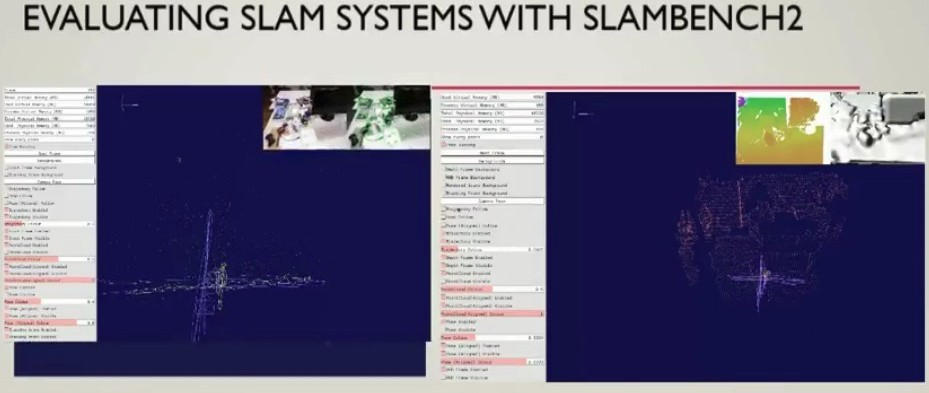
\includegraphics[height=6.0cm]{img/cap4/slambench.jpg}}
\end{center}
\caption{captura de la herramienta SLAMBENCH2.}
\end{figure}

Para medir el rendimiento de algoritmos SLAM se puede utilizar un framework para cuantificar la calidad de los resultados teniendo en cuenta exactitud, tiempo de ejecución, uso de memoria y consumo de energía. Esta información puede ser visualizada gracias a su interfaz gráfico.
Además SLAMBench ofrece una plataforma con grandes posibilidades para investigaciones futuras ya sea para diseño de algoritmos como optimizaciones a nivel de implementación. Es una herramienta multiplataforma y se puede utilizar en PCs de sobremesa, portátiles y móbiles. Algunos benchmarks se han obtenido con Ubuntu, OS y Android.
También puede ser utilizado con CUDA.
SLAMBench proporciona, entre otras métricas, medidas de exactitud del algoritmo utilizado. Las medidas de exactitud son determinadas comparando datos estimados con los datos ground-truth.
Absolute Trajectory Error (ATE) y Relative Pose Error RPE son utilizadas para medir la exactitud de la trayectoria. Estas métricas de trayectoria junto con una métrica de mapeo, Reconstruccion de Error , proporcionan comparaciones cuantitativas para varios algoritmos.

ATE y RPE son calculadas en tiempo de ejecución, con un alineamiento mínimo entre la primera posición más cercana de ground-truth y la posición estimada ( en términos de timestamp). Ya off-line, técnicas más complejas de alineamiento pueden ser usadas para comparar técnicas densas y semidensas cuando el mapeo de escalas no funciona. RER se calcula mediante la ejecución del algoritmo Iterative Closest Point (ICP) de los modelos de la nube de puntos de la reconstruncción y del ground truth. Como este proceso consume mucha CPU esta evaluación es tambien ejecutada off-line.

Otras métricas que proporciona SLAMBench es el consumo de energía ,utilización de memoria, velocidad de proceso por frame.

Interface de usuario modular: SLAMBench tambien permite elegir entre diferentes sistemas de interfaz de usuario. Métricas de evaluación pueden ser cambiadas y customizadas, así como el interfaz de usuario gráfico (GUI), mientras mantiene independencia de los datasets y algoritmos. Por ejemplo, el visualizador nativo está basado en la librería Pangolin , puede ser reemplazado por un visualizador ROS.

SLAMBench está siendo un componente muy importante en robótica y Sistemas de Realidad Aumentada (AR). Aunque un gran número de algoritmos SLAM han sido presentados, no se ha investigado lo suficente para tratar de unificar el interface de estos algoritmos, o realizar comparaciones de todas sus capacidades en conjunto. Esto presenta un problema ya que diferentes aplicaciones SLAM pueden tener diferentes requisitos funcionales y no funcionales. Por ejemplo, una solución para Realidad Aumentada desarrollada para móviles tendría que optimizar el consumo de energía, mientras que otra solución diseñada para vehículos de navegación autónoma estaría enfocada a funcionar con la mayor exactitud posible. SLAMBench2 es un framework de evaluación que compararía sistemas SLAM actuales y futuros, utilizando una lista extensible de datasets, mientras utiliza una lista comparable de métricas de rendimiento. Se podrían utilizar una gran variedad de algoritmos de SLAM y datasets como ElasticFusion, ORB-SLAM2, OKVIS y tambien se podría integrar con nuevos algoritmos y datasets. SLAMBench2 es un software que está disponible de manera pública. 

\item \textbf{The Kitti Vision Benchmark Suite }

Es un conjunto de aplicativos que utilizan mapas y secuencias grabados desde la plataforma de coches autónomos Annieway para crear nuevos desafíos o retos en las tareas comparativas o benchmarking de visualslam.\cite{Geiger2012CVPR}
Están investigando en varios campos como: vision stereo, flujo optico, odometría, detección de objetos en 3D y seguimiento de objetos 3D.
La exactitud de los conjuntos de datos ground truth es medida gracias al scanner laser Velodyne y a los sistemas de localización GPS con los que van equipados sus coches autónomos.
Los datasets han sido grabados en la ciudad de Karslruhe.
Además de proporcionar todos los datos en formato raw, para cada uno de sus benchmarks, también proporcionan una metrica de evaluación y una web de evaluación de métricas. En experimientos preliminares se ha comprobado que métodos que obtienen una puntuación alta en algunos benchmarks, cuando son aplicados al mundo real obtienen unos resultados por debajo de la media. El objetivo es reducir esta tendencia y completar los benchmarks existentes proporcionando benchmarks en el mundo real con dificultades novedosas para la comunidad. 

Un ejemplo podría ser el benchmark de odometría, que consiste en 22 sequencias stereo, grabadas en formato png. En el dataset se proporcionan 11 secuencias con trayectorias ground truth para entrenar y 11 sequencias sin ground truth para evaluar. Para este benchmark se pueden proporcionar reusltados usando una cámara o un sistema de cámaras estereo.
La única restricción que se impone es que el metodo deber ser totalmente automático (no se permite el etiquetado manual de cierre de bucle) y que el mismo conjunto de parámetros es usado para todas las secuencias.
Para todas las secuencias de test, su evaluador estima los errores de traslación y rotación. En una tabla de evaluación se establece un ranking de métodos de acuerdo con la media de esos valores, donde los errores son medidos en porcentaje para la trasalación y en grados por metro para la rotación.
\begin{figure}[H]
\begin{center}
\subfigure[]{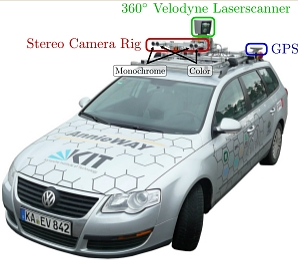
\includegraphics[height=6.0cm]{img/cap4/kittiCar.png}}
\end{center}
\caption{Coche autónomo Annieway utlizado con Kitti.}
\end{figure}

\end {enumerate}


\section{Comparativa de los algoritmos más representativos} 
A continuación se presenta una tabla que muestra las características principales de cada algoritmo. Esta tabla es similar a la que aparece en \cite{Perdices17} pero en este caso se ha añadido el algoritmo DSO.

\begin{center}
% \begin{tabular}{||c c c c c c c c||} 
\begin{tabular}{ |m{2.5cm} | m {1.5cm}| m {1.7cm}| m {1.7cm} | m {1.7cm}| m {1.7cm}| m {1.7cm}| m {1.7cm}| }
 \hline
 Funcionalidad & Mono-SLAM & PTAM & ORB-SLAM & LDSO  \\ [0.5ex] 
 \hline\hline
 Probabilístico & Sí & No & No & No \\ 
 \hline
 Hilos de ejecución & 1 & 2 & 3 & 2\\
 \hline
 Emparejamien-to & Parches & Parches & ORB & Métodos directos \\
 \hline
 Puntos 3D con incertidumbre & No & No & No & Sí\\
 \hline
 Mapa inicial & Dado & Homograf. & Homog. /Matriz F. & Incerti-dumbre \\ [1ex] 
 \hline
 \textit{Keyframes} & No & Sí & Sí & Sí  \\ [1ex] 
 \hline
 Puntos en mapa & Cientos & Miles & Miles & Miles \\ [1ex] 
 \hline
 Mapa denso & No & No & No & Semi-denso\\ [1ex] 
 \hline
 Gestión de mapas grandes & No & No & Sí & Sí \\ [1ex] 
 \hline
 Relocalización & No & Sí & Sí & No\\ [1ex] 
 \hline
 Rechazos de espurios & No & No & Sí & No\\ [1ex] 
 \hline
 Cierre de bucle & No & No & Sí & Sí\\ [1ex] 
 \hline
\end{tabular}
\end{center}
\clearpage
%\flushbottom
\newpage
\pagebreak










 %3
\newpage
\newpage
%\chapter{Descripción} \label{cap:Herramienta SLAMTestbed}
\chapter{Herramienta SLAMTestbed} \label{cap:Herramienta SLAMTestbed} %chapter 4
%\setcounter{section}{4}
En este capítulo se detalla el diseño y la implementación de SLAMTestbed, una aplicación herramienta diseñada y creada para comparar cuantitativamente algoritmos SLAM. El diseño de algoritmos SLAM, y de Visual SLAM en particular es todavía una disciplina abierta en periodo de expansión y cuenta cada vez con un mayor número de aplicaciones reales, entre las que destaca la navegación de vehículos autónomos o las aplicaciones de realidad aumentada. Existe un gran número de algoritmos, por lo que se necesitan herramientas que  permitan medir la precisión, robustez y velocidad de cada algoritmo.

Comenzaremos explicando el diseño de la herramienta SLAMTestbed desde un punto de vista de Caja Negra, explicando sus entradas y sus salidas. Se continuará con la explicación de su diagrama de bloques y se finalizará profundizando en cada uno de los componentes principales de la herramienta, es decir los distintos módulos que permiten calcular el Registro Espacial ( Escala, Traslación y Rotación) y el Registro Temporal (interpolación de frecuencias y cálculo de \textit{Offset} o Desplazamiento Temporal) entre dos secuencias de posiciones y orientaciones 3D.

\section{Diseño}

En esta sección no entraremos en los detalles de la implementación de la herramienta SLAMTestbed, si no que lo trataremos como una \textit{caja negra}.
En la entrada del sistema tendremos dos secuencias de puntos 3D.
Las secuencias procesados por esta herramienta serán ficheros de texto cuyos registros tendrán los siguientes 8 campos:

\textit{Timestamp, X, Y, Z, qx,qy,qz,qw}

Uno de los \textit{dataset} será la verdad absoluta, y el segundo\textit{dataset} será la posición y orientación en 3D obtenidos tras aplicar un algoritmo Visual SLAM, correspondiendo cada registro del \textit{dataset} con una posición de la cámara.
Una vez procesados los dos \textit{datasets} por la herramienta, obtendremos como salida, las transformaciones estimadas por la herramientas entre la verdad absoluta y las posiciones y orientaciones calculadas por el algoritmo de SLAM. Además, se obtendrá un conjunto de estadísticos que miden el error cometido en las estimaciones de SLAM y así poder medir la precisión de los algoritmos.


\begin{figure}[H]
\begin{center}
\label{fig:Open File}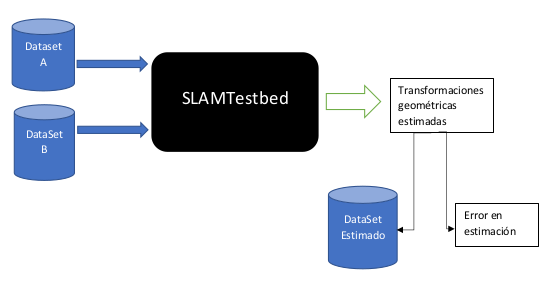
\includegraphics[height=8.0cm,width=14.0cm]{img/cap5/Esquema_TFM_CajaNegra2.png}
\hspace{0.5cm}
%\subfigure[]{\label{fig:LG_hombot}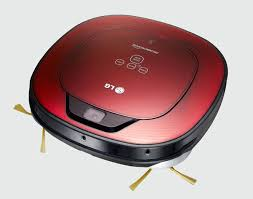
\includegraphics[height=6.0cm]{img/cap2/LG_hombot.jpg}}
\end{center}
%\caption{Robot Dyson 360 Eye (a) Robot Roomba 966 (b) Robot Hombot de LG (c).}
\caption{ El diseño de Caja Negra de la herramienta SLAMTestbed. }
\end{figure}

%\section{Diseño de caja Blanca}
Una vez explicadas las entradas y salidas de la aplicación ahora explicaremos
con más detalle la implementación de la herramienta SLAMTestbed. 

El objetivo principal de la herramienta desarrollada es calcular el error existente entre una secuencia con las posiciones y orientaciones 3D verdaderas (\textit{dataset A}) y la trayectoria calculada por el algoritmo de SLAM (\textit{dataSet B}). Para que esto sea posible, necesitaremos antes eliminar algunas variables que no permiten comparar directamente las dos trayectorias, como son la escala, el offset temporal y la transformación en 3D entre ellas. Por ello, necesitaremos calcular un nuevo \textit{dataset} (estimado), que sea comparable con el \textit{dataset A}. 

Las principales funciones o módulos utilizados para obtener el \textit{dataset} estimado son:

\begin{description}
\item [Cálculo de PCA]:

El análisis de componentes principales (o PCA), nos permitirá reducir los dos  \textit{dataSets} a sus componentes principales, lo que posibilita estimar la escala y el offset existente entre ellos.
\item [Estimación de Escala]: 

Estima la diferencia de escala entre los dos \textit{datasets} a partir de los datos proporcionados en el cálculo de componentes principales.
\item [Estimación de Offset temporal]: 

Con este módulo podremos hallar la diferencia entre marcas de tiempos de los 2 \textit{datasets}, ya que pueden haber comenzado en periodos de tiempo distintos.
\item [Interpolación para igualar frecuencias de muestreo]: 

Con la interpolación podremos igualar en frecuencias los dos \textit{datasets}, en caso de que éstas sean distintas, que es lo habitual por que el algoritmo SLAM genera estimaciones a diferente ritmo del que vienen las muestras de la secuencia con verdad absoluta.

\item [Operaciones de Registro para estimar la Rotación y Traslación]: 

Permitirá estimar las traslación y rotación existentes entre el \textit{dataset A} y el \textit{dataset B} y llevarlas así al mismo sistema de referencia espacial, donde ya son directamente comparables.
\end{description}


%\begin{figure}[H]
\begin{figure}
\begin{center}
\label{fig:Open File}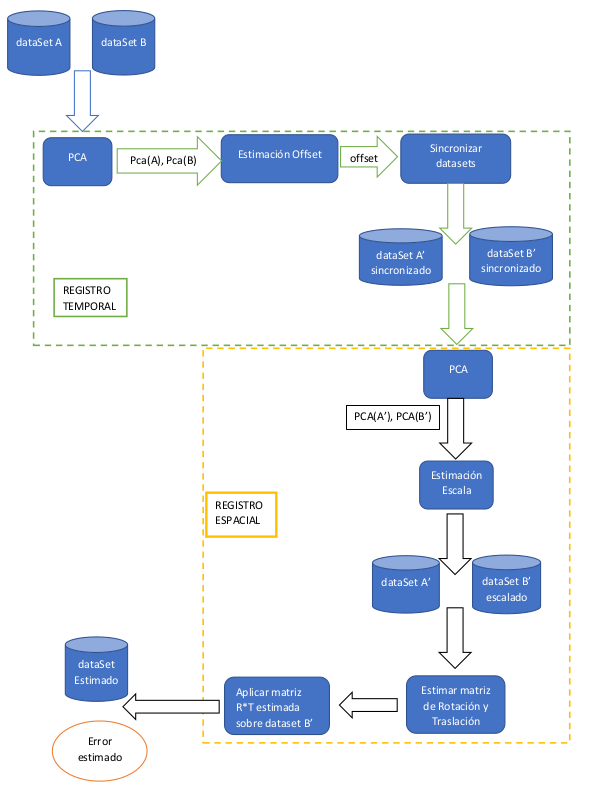
\includegraphics[height=18.0cm,width=12.0cm]{img/cap5/EsquemaTFM_CajaBlanca_Transformaciones4.png}
\hspace{0.5cm}
%\subfigure[]{\label{fig:LG_hombot}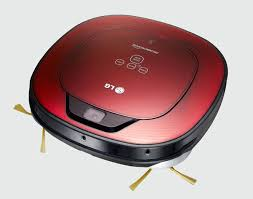
\includegraphics[height=6.0cm]{img/cap2/LG_hombot.jpg}}
\end{center}
%\caption{Robot Dyson 360 Eye (a) Robot Roomba 966 (b) Robot Hombot de LG (c).}
\caption{ Diagrama de bloques de la herramienta SLAMTestbed }
\end{figure}

La explicación al flujo de datos seguido en la Figura 4.2 es el siguiente:


Primero se calcula la descomposición en componentes principales (PCA) para cada uno de los \textit{datasets} obteniendo como resultado \textit{dataSet A'} y \textit{dataSet B'}. Posteriormente se estima el \textit{offset} o desplazamiento de tiempo que exista entre las 2 secuencias de datos o \textit{datasets}. Corrigiendo el offset en el \textit{dataset B}, sumando el valor del \textit{offset} calculado a los valores de tiempo del \textit{dataset B} así las dos secuencias tienen ya el mismo origen de tiempos. Una vez tengamos calculado el offset, unificaremos las frecuencias de los 2 \textit{datasets} mediante interpolación. En este proceso de interpolación se generarán nuevas muestras para los \textit{datasets'}.
Cuando tengamos unificada la frecuencia para los dos \textit{datasets}, obtendremos de nuevo PCA de ambos \textit{datasets} y podremos obtener la escala.
Posteriormente estimaremos la transformaciones de rotación y traslación para pasar del \textit{dataset A} al \textit{dataset B}. Aplicaremos dichas transformaciones sobre el \textit{dataset A}, para obtener un nuevo \textit{dataset}, el \textit{dataset} Estimado que pintaremos en pantalla de color rojo.

A continuación se explicarán con más detalle cada uno de estos módulos.


\section{Estimador PCA y Cálculo de Escala}
    En análisis de componentes principales (\textit{PCA} según sus siglas en inglés) es el algoritmo más utilizado para reducir las dimensiones de un conjunto de datos. Como resultado de aplicar PCA sobre un conjunto de datos, obtendremos un nuevo conjunto de datos en términos de nuevas variables no correlacionadas, que denominaremos componentes principales.

    Las componentes principales se ordenarán por su Varianza, de esta forma la primera componente principal será la que mayor varianza tenga e identificará un eje. Un segundo eje ortogonal al primero vendrá definido por la segunda componente principal e identificará la segunda mayor varianza. Finalmente obtendremos un tercer eje ortogonal a los dos primeros, definido por la tercera componente principal que identificará la tercera mayor varianza.

    En nuestro caso, este análisis nos permitirá obtener el tamaño de cada \textit{dataset} en cada una de sus componentes (x,y,z)
	Este análisis es necesario puesto que los ejes de las dos secuencias de entrada no tienen porqué coincidir. Por ello, con los valores obtenidos con PCA podremos generar dos nuevos \textit{datasets} cuyos ejes sean comparables, es decir que estén alineados. A partir de los nuevos \textit{datasets} generados podremos calcular la diferencia de tiempos entre los dos \textit{datasets} y posteriormente la escala entre ambos.
 
	Se implementan dos métodos de cálculo de PCA, el primero es realizando una descomposición Eigen \textit{eigenDecomposition}, el segundo utilizando el método SVD (utilizando la librería Eigen), que describiremos a continuación en pseudocódigo.

	\begin{lstlisting}[frame=single]
		# Obtener el valor medio de cada componente
		mX = media (dataset.x)
		mY = media (dataset.y)
		mZ = media (dataset.z)

		#restar la media a cada componente x, y z

		dataset2.x = dataset.x - mX
		dataset2.y = dataset.y - mY
		dataset2.z = dataset.z - mZ
        
        #Calcular el nuevo dataset

		cov = obtenerMatrizCovarianza(dataset2)
		svd = CalularSVD(cov )
		pca =  Matriz V del resultado svd
		datasetResultado = dataset * Matriz (svd.V)

	\end{lstlisting}

    Una vez que los ejes de ambos \textit{datasets} sean comparables, podremos calcular la diferencia de escala entre los dos \textit{datasets}, lo que permitirá igualar la escala entre los \textit{datasets} obteniendo así el primer paso del registro espacial. El algoritmo utilizado está basado en la utilización de los valores singulares de cada \textit{dataset}, como se muestra en el siguiente pseudocódigo:

        
	\begin{lstlisting}[frame=single]
		S1 = svd(dataSet1).valoresSingulares
		S2 = svd(dataSet2).valoresSingulares
		scalaX = S2(0)  / S1(0)
		scalaY = S2(1)  / S1(1)
		scalaZ = S2(2)  / S1(2)
	\end{lstlisting}

\section{Estimador Offset Temporal}

Este módulo es necesario puesto que los \textit{datasets} pueden tener un desfase en su inicio, incluso aunque hayan sido obtenidos a partir de la misma secuencia, debido a la propia implementación de los algoritmos SLAM. El método principal utilizado para estimar el offset se realiza mediante el cálculo de la Correlación Cruzada. 
Este método conlleva una gran carga para la CPU ya que incluye múltiples cálculos para interpolar y calcular la correlación cruzada entre los dos \textit{datasets}. Este algoritmo es iterativo y utilizaremos un dataset como base de tiempo fijo y otro dataset B que se deslizará en el tiempo desde -T hasta +T en pequeños incrementos de tiempo, pasos o \textit{steps} en cada iteración, calculando para cada paso la correlación cruzada entre el \textit{dataset} deslizante y el \textit{dataset} original (que se mantiene fijo en el tiempo). 
En cada iteración del algoritmo se calculará la correlación para un paso determinado, almacenando la memoria el paso cuya correlación sea mayor, lo que nos indicará el offset temporal entre las dos secuencias. Para ello calcularemos la interpolación para los puntos 3D orientados que estén dentro del rango temporal de los dos \textit{datasets}. Una vez interpolados los puntos 3D comunes de las dos series temporales tendremos dos series nuevas, para las cuales calcularemos la correlación cruzada aplicando el algoritmo clásico para dos series temporales. Pero antes, y como cada serie temporal tiene 3 coordenadas (x,y,z para cada punto 3d), debemos transformar estas 3 coordenadas en un sólo valor para cada punto 3D de cada serie, para ello tendremos que calcular la distancia al origen de todo punto 3D, y por tanto la correlación cruzada se calculará sobre los dos \textit{datasets} convertidos a distancias al origen de coordenadas.
Para un punto 3d (x,y,z), la distancia 3d respecto al origen se calculará:
\begin{center}
	\begin{math}
	\sqrt{(x-0)^2 +(y-0)^2+(z-0)^2}
	\end{math}
\end{center}

\begin{figure}[H]
\begin{center}
\label{fig:opciones de View}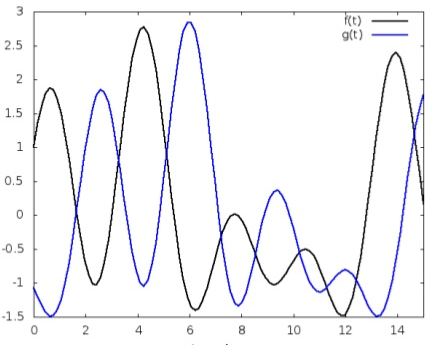
\includegraphics[height=8.0cm,width=12.0cm]{img/cap5/correlacionCruzada2.png}
\hspace{0.5cm}

\end{center}

\caption{Gráfico que muestra el desfase del offset entre dos series temporales y el resultado de la correlación cruzada.}
\end{figure}
	                                
	\begin{lstlisting}[frame=single]
	dataA(d) = CalcularDistanciaAlOrigen( dataSetA(x,y,z))
	dataB(d) = CalcularDistanciaAlOrigen( dataSetB(x,y,z))
	mA = CalcularMedia(dataA)
	mB = CalularMedia(dataB)

	Para cada fila

   		sx = dataA(i) - mA

   		sy = dataB(i) - mB

   	denom = sqrt(sx*sy);
   	step = 0.01
   	Desde i=-T hasta i = T
   		Si ( dataB.t < dataB.t )
			j=j+1
    		continuar

    	sino si (dataB.t > dataA.t)
    		i=i+1
    		continuar

    	sino si (dataB.t == dataA.t)
    		sxy=(dataA -mA) * (dataB-mB)
        	i++
        	j++


   

   r = (sxy) / denom;

   r= fabs(r);
    \end{lstlisting}



\section{Interpolador temporal}

	El módulo de interpolación se utiliza para sincronizar a igual frecuencia 2 secuencias, cuyas frecuencias de muestreo no sean iguales, algo que es común entre los algoritmos de SLAM.
	En este proceso de interpolación se generarán nuevos registros en el \textit{dataset} a partir de la interpolación de muestras entre dos marcas de tiempo.
	Este interpolador puede configurarse para que tenga distintos comportamientos:
    \begin{enumerate}
	 
	 \item{\textbf{Interpolación a la frecuencia menor}} de los dos \textit{datasets}. Aunque se generarán nuevos registros sincronizados por interpolación, en general se perderán registros del dataset de mayor frecuencia.

	 \item{\textbf{Interpolación a la frecuencia mayor}} de los dos \textit{datasets}. En este caso se generarán nuevos registros para el dataset de menor frecuencia.

	 \item{\textbf{Interpolación a frecuencia común}}, en este caso, los dos \textit{datasets} se deberán sincronizar a la frecuencia deseada por el usuario.
	 \end{enumerate}

	 En los tres casos, la interpolación se realiza sobre las secuencias temporales de los 2 \textit{datasets}, pero además se calcula la interpolación para las coordenadas X,Y,Z de cada punto 3D y valores (qx,qy,qz,qw) de cada cuaternio. La función \textit{slerp} de la librería Eigen nos permite calcular la interpolación entre cuaternios, viene de la abreviatura de la definición en inglés \textit{Spherical Linear intERPolation}, creada para animaciones de rotaciones 3D utilizando cuaternios.


	 La fórmula para la interpolación lineal utilizada sería:

	 \begin{center}
	 \begin{math}
		y-y2= (t-t2)*\frac{y3-y2}{t3-t2}
	 \end{math}
	 \end{center}

	 Donde t sería el nuevo valor de tiempo para el cual deberíamos interpolar los nuevos valores de las cordenadas X,Y,Z. 
	 Los valores t3,y3 hacen referencia al valor de la secuencia en t+1
	 Los valores t2,y2 hacen referencia al valor de la secuencia en t-1

	 %double y= y2 + (x-x2)*((y3-y2)/(x3-x2));
	 %double y2= (B.row(contB-1))(1);
	%double x = (A.row(contA-1))(0);t
	%double x2= (B.row(contB-1))(0);t2
	%double y3= (B.row(contB))(1);
	%double x3= (B.row(contB))(0);t3
	 



\section{Registro Espacial}
Una vez modificados los dos \textit{datasets} para que tengan la misma escala y la misma frecuencia de muestreo y el mismo origen temporal, el siguiente paso es obtener la rotación y la traslación que existe entre ellos. Esta matriz servirá para transformar el segundo \textit{dataset}, y así poder calcular el error existente en la trayectoria obtenida por el algoritmo de SLAM.
Los pasos necesarios para realizar este registro espacial son los siguientes:

\textbf{Hallar la matrices de rotación y traslación} .

	El algoritmo desarrollado para esta funcionalidad sería el siguiente:
    \begin{lstlisting}[frame=single]
    # Hallar los centroides para las coordenadas X,Y,Z 
    	centA = centroides (A)
    	centB = centroides (B)
    

    # Restar los centroides a sus respectivas matrices
      	A= A-centA
      	B= B-centB
    
    # Calcular el producto de las matrices
    	H = A.traspuesta * B

    # Obtener valores singulares de la matriz H
    	S,U,V = svd(H)
    
    # Obtener la matriz de Rotacion
      	R = V*U.traspuesta

    # Obtener la matriz de Traslacion
    	t= -R * centA + centB;  
    \end{lstlisting}

\textbf{Transformar un \textit{dataset} aplicando las matrices de Rotación y Traslación estimadas}

Este método tomará un \textit{dataset}, lo multiplicará por la matriz de rotación y le sumará la matriz de traslación.

\textbf{Transformar los cuaternines aplicando la matriz Rotación.}

Con este método conseguimos transformar los cuarternios del \textit{dataSet A} al \textit{dataSet B}. Para ello convertiremos la matriz de rotación en un cuaternio que llamaremos "q". Por último multiplicaremos cada cuaternio p de la siguiente forma.
\begin{center}
		\textit{q * p * q.inverso }
\end{center}

\textbf{Estimar las matrices de rotación y traslación mediante la técnica de RANSAC.}
Estimaremos las matrices de Rotación y Traslación utilizando los datos de los dos \textit{datasets}, eliminando primero los puntos espúreos (outliers) mediante el algoritmo RANSAC \cite{Fischler:1981:RSC:358669.358692}.
Se ha elegido RANSAC por que permite estimar la matríz R*T entre ambas secuencias con robustez, de modo que la estimación es fiable.



El algoritmo seguido ha sido el siguiente:
    \begin{lstlisting}[frame=single]
	Mientras n < MaxIteraciones hacer
		Seleccionar n inliers
		Estimar una primera matriz de R*T
		aplicar R*T sobre subconjunto NoInliers
		Si el error < threshhold
			agregar candidato a inliers
		aplicar RT sobre inliers, NoInliers
		medir el error 
		seleccionar menor error
		incrementar iteraccion
	Devolveremos las matrices de R*T con menor error
	\end{lstlisting}
	        
   

\section{Cálculo de Estadísticas}

Este bloque mide las diferencias entre dos secuencias pero cuando una de llas es la de posiciones verdaderas y la otra es de posiciones estimadas, entonces esas diferencias se interpretan correctamente como el error en las posiciones etimadas.

Para medir el error cometido entre el \textit{dataset} con posiciones orientadas verdaderas y el \textit{dataset} Estimado utilizaremos el módulo de Cálculo de Estadísticas.
Este módulo permite calcular distintos estadísticos, como el error medio, mediano, máximo y mínimo, así como el Error Cuadrático Medio (Root Mean Square Error).
Cuanto menores sean estos valores, mejor será la estimación.

De entre estos estadísticos, el que mejor determina la calidad de la trayectoria estimada por los algoritmos de SLAM es el error cuadrático medio, puesto que penaliza los errores demasiado grandes más que otros estadísticos, algo que es determinante en los algoritmos de SLAM. Cuanto más próximo a 0 sea el valor del RMSE, mejor será la estimación. Si conseguimos un RMSE con valor 0 significa que los datos estimados coinciden con los datos que hemos tomado como verdad absoluta o \textit{groundtruth}.

El RMSE se calcula de la siguiente forma:
\begin{center}
\begin{math}
RMSE =\sqrt{\sum{( g - e)^2}/N}
\end{math}
\end{center}

donde g es el dataset \textit{groundTruht}

      e es el dataset Estimado

      N es el número de elementos de los datasets

Otro valor de medida de error calculado es la distancia angular entre 2 rotaciones, que nos sirve para medir el grado de error entre la orientación real y la orientación estimada, para ello convertimos la matriz de rotación estimada en un cuaternio usando la libreía Eigen.

Los pasos para medir este error angular sería:
\begin{lstlisting}[frame=single]
convertir matriz de rotacion en cuaternio  q
convertir matriz de rotacion estimada en cuaternio p
normalizar cuaternios q y p
myAngularDistance=p.angularDistance(q);

\end{lstlisting}

En caso de no conocer la matriz de rotación de la secuencia verdadera, el vector q será igual a (1,0,0,0).








\section{Interfaz Gráfico de Usuario}
Para la herramienta SLAMTestbed también se ha diseñado y creado un Interfaz de Usuario Gráfico (\textit{Graphic User Interface}) que permita pintar los puntos 3D de cada \textit{dataset} en pantalla, así como invocar comandos (a través de clicks de ratón) para ejecutar los distintos módulos que contiene la herramienta.

Esto permite medir la exactitud de los resultados de la aplicación de un algoritmo con los resultados de otro algoritmo o comparar varios resultados de un mismo algoritmo en el que se han aplicado distintos parámetros de ejecución.

Este interfaz gráfico de usuario de 3 dimensiones ha sido desarrollado en C++ con el entorno QT , OpenGL y la librería Eigen. 

La librería Eigen \footnote{https://eigen.tuxfamily.org/dox/GettingStarted.html} es una librería \textit{Open Source} realizada en C++, para cálculos de Álgebra lineal, operaciones con Matrices y vectores, Transformaciones Geométricas. 

OpenGL\footnote{https://www.opengl.org/} es un API estandar y se ha utilizado en este proyecto para todo el tratamiento en gráficos 3D, pero apenas proporciona soporte para GUI, es por ello, por lo que se decidió incorporar como herramienta de desarrollo el \textit{framework} QT. 

QT \footnote{https://www.qt.io/developers/} es un framework de desarrollo en C++, con el cual se ha podido diseñar y desarrollar el interfaz de usuario de SLAMTestbed. Además, contiene el módulo QTOpenGL que permite integrar facilmente código OpenGL con aplicaciones QT.

La aplicación software muestra al usuario un interfaz gráfico que permite leer un archivo de datos con puntos 3D y mostrarlo en pantalla como una nube de puntos 3D (Figura 4.5). Este archivo podríamos denominarlo groundTruth.
Con el ratón podremos girar en 3 dimensiones la nube de puntos, acercarnos  (Zoom in) o alejarnos (Zoom Out), así como leer un segundo conjunto de puntos 3D y estimar las transformaciones ( rotaciones , traslaciones, escala etc) que existen entre ellos. El conjunto de datos resultante tras aplicar las estimaciones será visualizado en pantalla como otra nube de puntos 3D.

\begin{figure}[H]
\begin{center}
\label{fig:Transformaciones versus Estimaciones}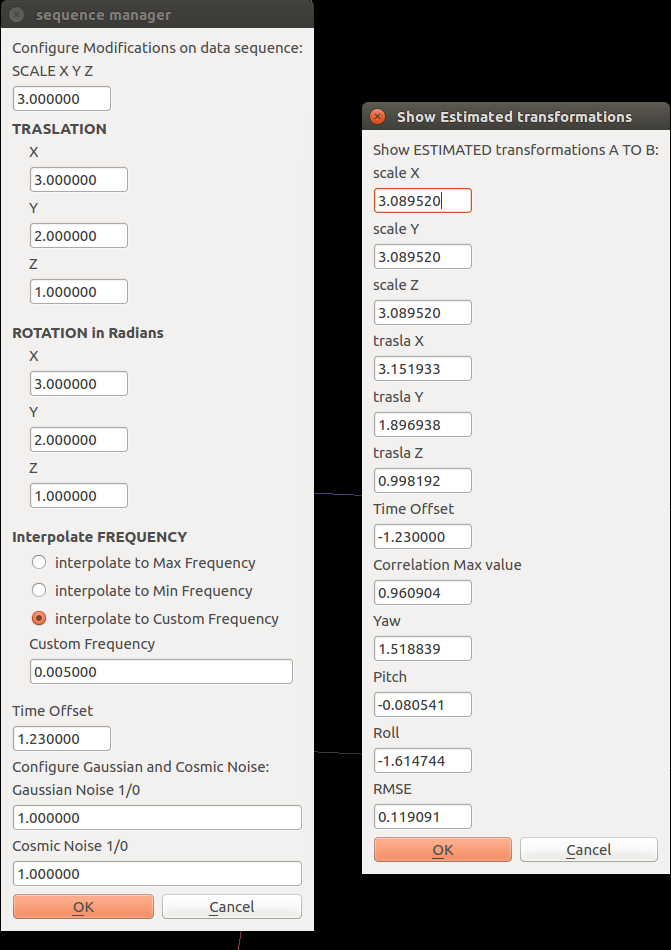
\includegraphics[height=12.0cm,width=8.0cm]{img/cap5/showTransformationsEstimated.png}
\hspace{0.5cm}
\end{center}
\caption{Transformaciones realizadas frente Transformaciones estimadas }
\end{figure}


\begin{figure}[H]
\begin{center}
\label{fig:opciones de View}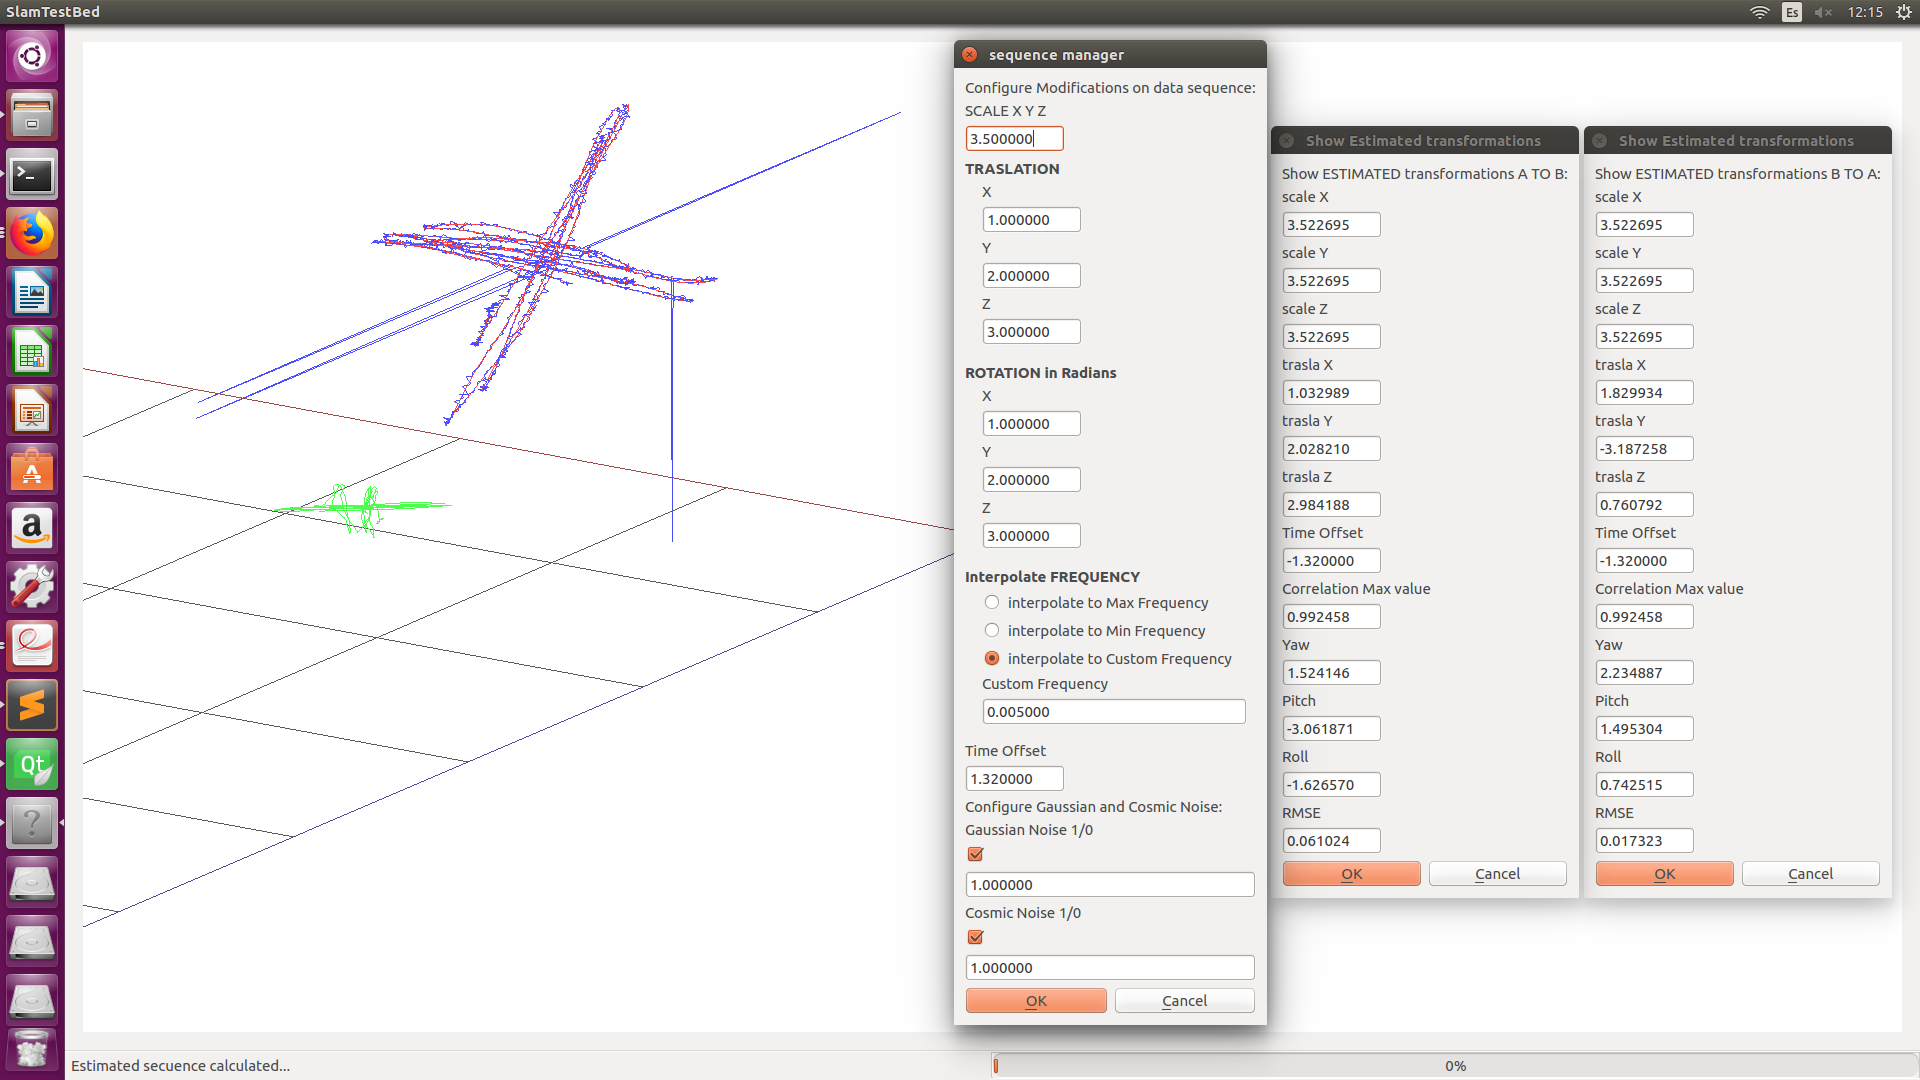
\includegraphics[height=10.0cm,width=15.0cm]{img/cap6/Escala_Trasla_Rota_Offset_Gauss_CosmicNoise_abba.png}
\hspace{0.5cm}

\end{center}

\caption{Gráfico que muestra los resultados de la estimación de un cambio de escala y traslación .}
\end{figure}

En la pantalla gráfica podremos ver tres \textit{datasets}. Los puntos 3D del primer \textit{dataset} \textit{groundtrouth} se pintarán en color verde, los puntos del \textit{dataset} a evaluar o \textit{dataset} transformado serán de color azul, y por último en color rojo estarán los puntos 3D del \textit{dataset} estimado.
En el caso de que el error entre los dos \textit{datasets} sea pequeño, los puntos 3D correspondientes al \textit{dataset} estimado solaparán con los puntos correspondientes a la verdad absoluta, lo que significará que la trayectoria calculada por el algoritmo de SLAM es cercana a la realidad y en este caso el punto estimado (en color rojo) quedará invisible. Además el GUI también muestra los valores de transformación estimadas (Figura 4.4)


%\clearpage

 %4
\newpage
\chapter{Experimentos} \label{cap:experimentos}
%\section{Conclusiones} \label{s:conclusiones}
%\setcounter{section}{5}
En este capitulo mostraremos las pruebas realizadas con la herramienta SLAMTESTBED.
Para comprobar los resultados podremos utilizar la ventana que muestra el resultado de las estimaciones una vez han terminado los cálculos. Gracias a la visualización gráfica de los datasets (incluido el dataset estimado) la evaluación de los resultados será más sencilla y fiable, ya que si los puntos 3D del dataset estimado no se aproximan al dataset destino, el desajuste entre los puntos 3d de ambos dataset será perceptible a simple vista.


Acontinuación mostraremos las pruebas realizadas para estimar las transformaciones para convertir el dataset A en el datasetB y viceversa, donde el datasetB se obtiene como resultados de aplicar el módulo transformador sobre el datasetA.
Se han realizado varias pruebas, en cada una de ellas se han activado un subconjunto de parámetros del módulo transformador, es decir que en una prueba se habrá modificado sólo la escala y un traslación , en otras pruebas se habrá realizado cambios en traslación y rotación , etc.

En cada captura de pantalla aparecerá de forma gráfica , el dataset original (en verde), el dataset transformado (en azul), y el dataset estimado (en rojo), junto con otras 3 pantallas que indicarán los valores de los parámetros de las transformaciones realizadas, y otras 2 pantallas con los valores de la estimaciones calculadas (tanto si la estimación ha sido calculada del datasetA al datasetB o del datasetB al datasetA).

\section{Módulo Transformador}
Esta herramienta poseé varios modulos accesibles desde el interfaz gráfico. Entre estos módulos podríamos destacar el \textbf{Módulo Transformador}.
Como se ha comentado anteriormente, el módulo Transformador permite realizar transformaciones sobre el conjunto de puntos 3D groundTruth, de tal forma que se obtendrá como resultado una segunda nube de puntos transformados. De esta forma se han podido realizar pruebas teniendo un sólo datasets para comprobar que los calculos estimados de Traslación , Rotación y escala son fiables y tienen un error mínimo.

Los diversos parámetros del módulo transformador serán accesible por el interfaz gráfico de la pantalla.

A continuación describiremos en detalle las transformaciones permitidas por la herramienta:

\textbf{Escala}. Permite modificar los datos de entrada a nivel de escala. La escala siempre será mayor que cero y se admitirán números con reales. Por defecto tendrá el valor de 1. 

\textbf{Traslaciones}. Se podrán definir traslaciones sobre cada uno de los 3 ejes de coordenadas. 
La traslación admite números reales positivos y negativos.

\textbf{Rotaciones}. Se podrán definir rotaciones sobre cada unos de los 3 ejes de coordenadas. El valor de cada rotación se insertará en Radianes. Los valores admitidos serán números reales tanto positivos como negativos. Para indicar rotaciones, los ángulos de rotación se incluirán en Radianes.

\textbf{Offset de tiempo}. Con el offset de tiempo podremos introducir un 'gap' en los valores de timestamp del fichero de entrada que más tarde podremos estimar. La exactitud del offset será de centésimas, es decir con 2 decimales.

\textbf{Interpolación}: El módulo de interpolación nos permitirá ajustar a la misma frecuencia los 2 datasets. Se podrán realizar 3 tipos de interpolación de los datos.
	Interpolación a la frecuencia máxima
	Interpolación a la frecuencia mínima
	Interpolación a frecuencia personalizada

\textbf{Ruido Gaussiano}: Una de las transformaciones que podremos aplicar sobre el conjunto de datos del groundtrouth es aplicar un ruido gaussiano a los datos transformados

\textbf{Ruido Cósmico}: Otra transformación a aplicar sobre los datos transformados es la incorporación del ruido cósmico


\section{Pruebas de transformaciones individuales}

En este apartado, mostraremos imágenes del módulo GUI, donde se han realizado varias pruebas de transformaciones indivicuales y se han estimado dichas transformaciones.
En todas las transformaciones se ha realizado la interpolación de frecuencias al valor 0.05 para ambos datasets.

\begin{figure}[H]
\begin{center}
\subfigure[]{\label{fig:opciones de View}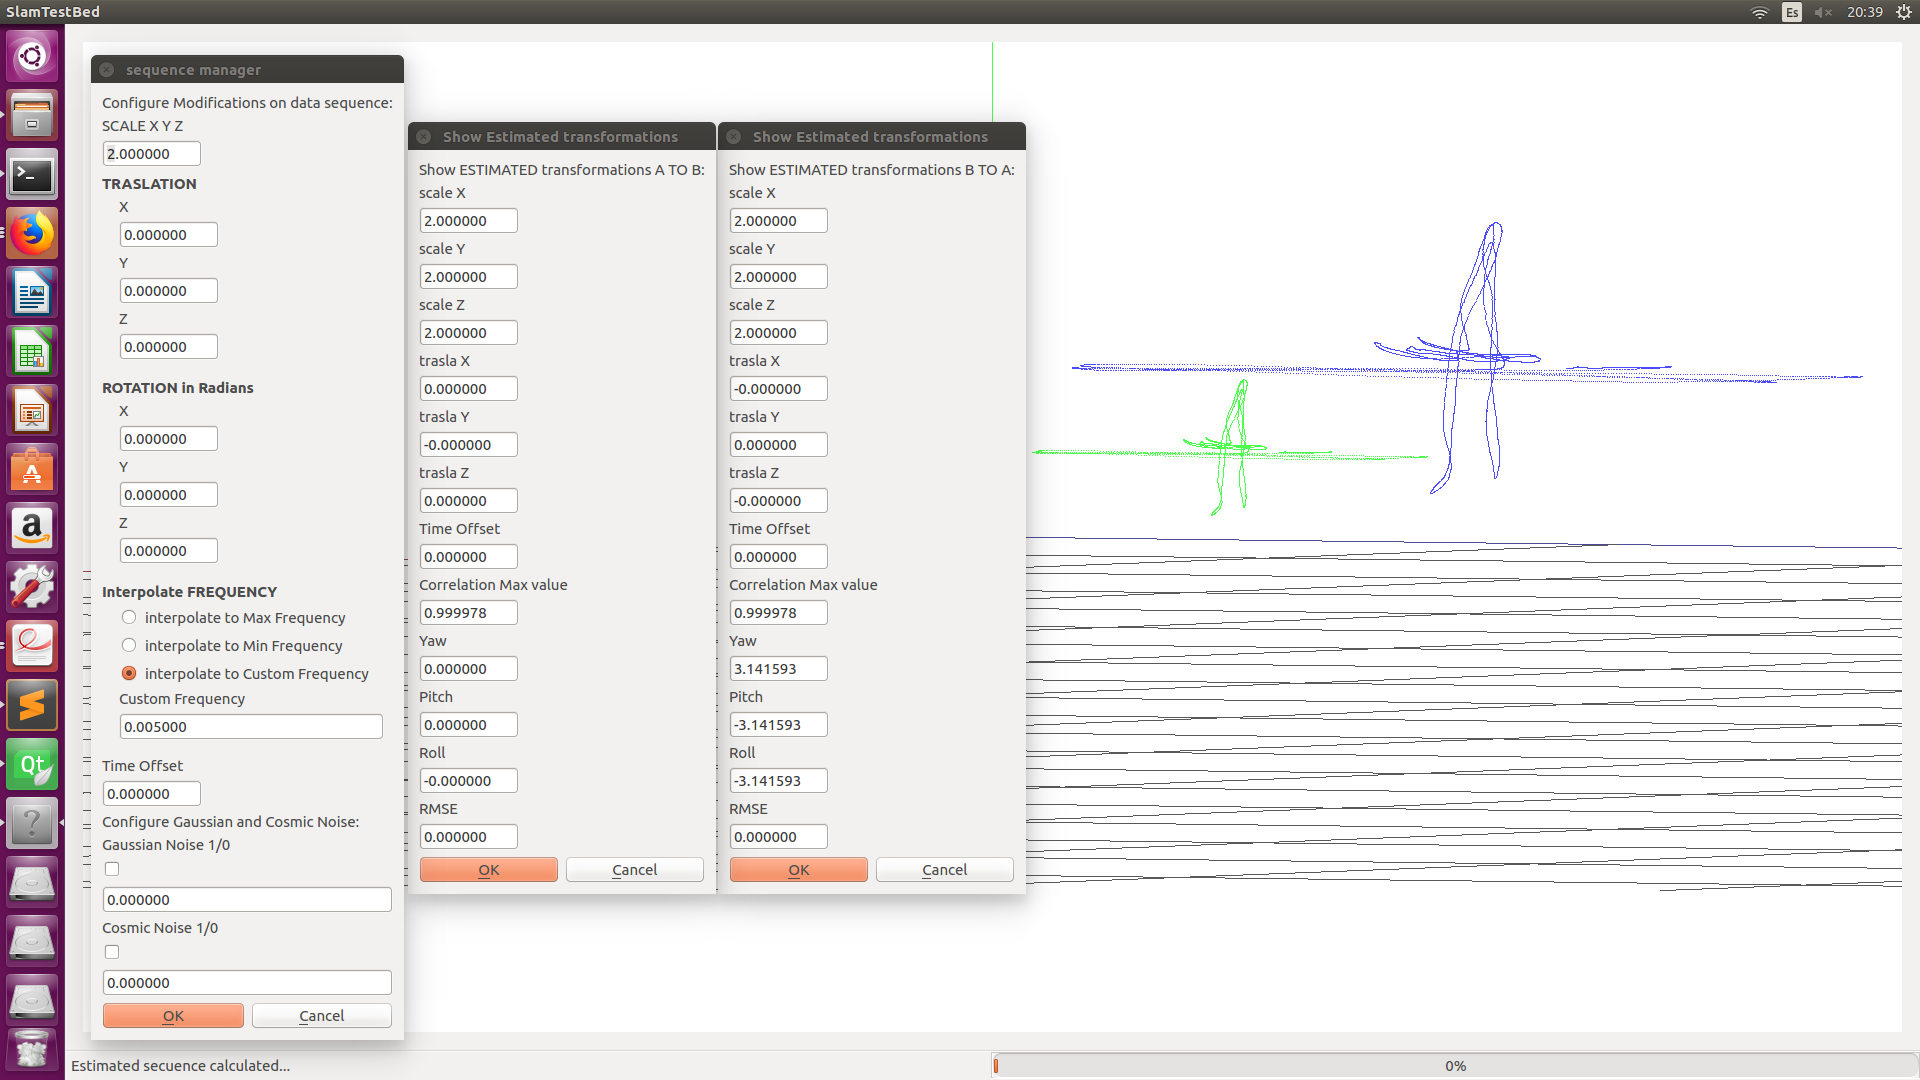
\includegraphics[height=10.0cm,width=15.0cm]{img/cap6/Escala_abba.png}}
\hspace{0.5cm}

\end{center}

\caption{Gráfico que muestra los resultados de la estimación tras una transformación de un cambio de escala.}
\end{figure}

El gráfico superior muestra los resultados de la estimación tras una transformación de un cambio de escala. Se aprecia en la captura de pantalla, como el dataset transformado es más grande que el dataset original. Como se puede observar el RMSE es 0.0 y el valor de la escala estimada coincide con el valor de la transformación de escala, en este caso es 2.0

\begin{figure}[H]
\begin{center}
\subfigure[]{\label{fig:opciones de View}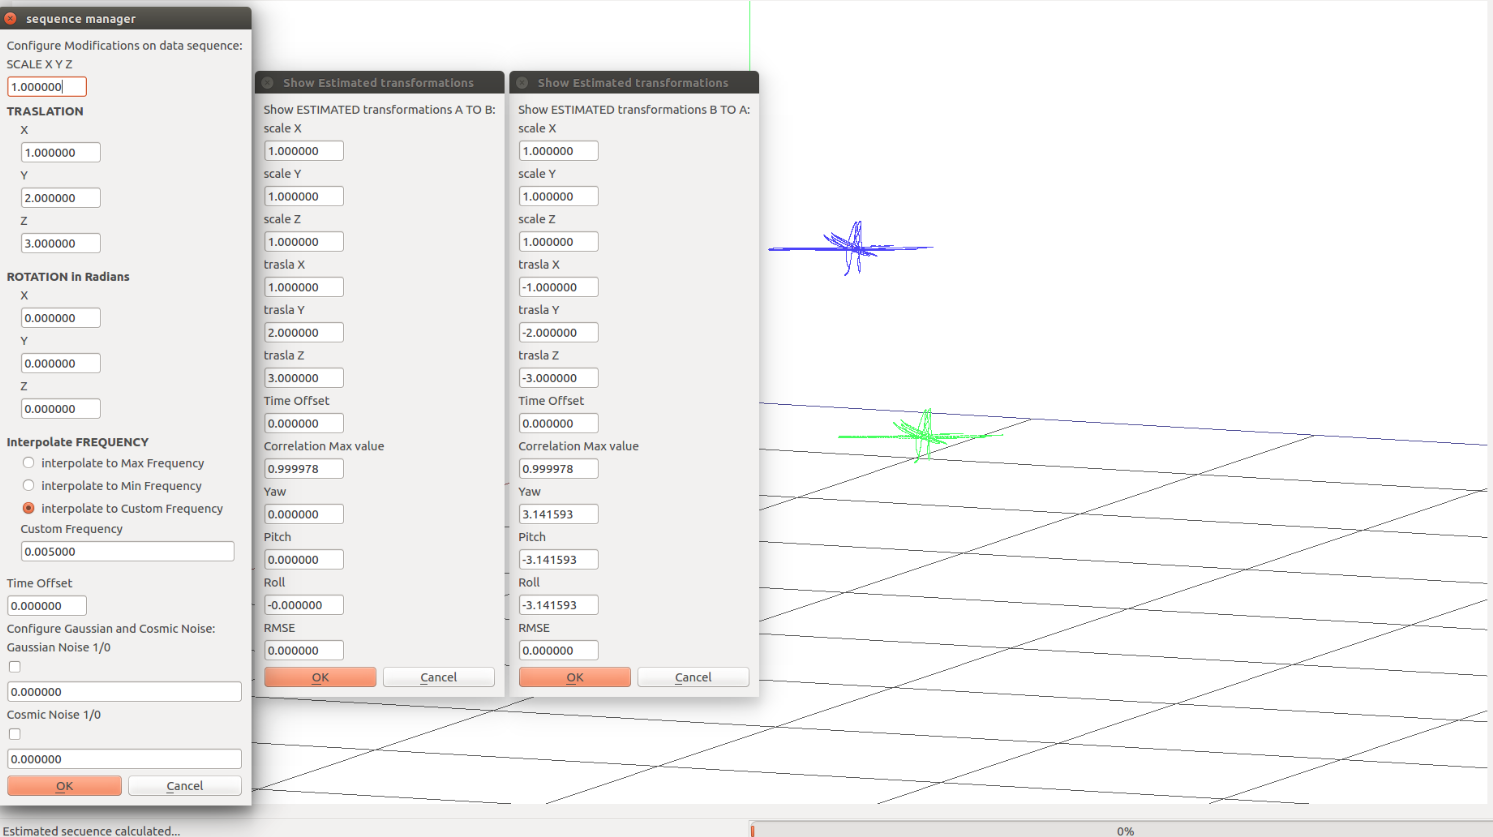
\includegraphics[height=10.0cm,width=15.0cm]{img/cap6/Traslation_abba.png}}
\hspace{0.5cm}

\end{center}

\caption{Gráfico que muestra los resultados de la estimación de un cambio de traslación.}
\end{figure}

La captura de pantalla superior muestra los resultados de la estimación tras realizar una traslación en el dataset original. Como puede observarse el RMSE es 0.0, y gráficamente el dataset transformado y estimado coinciden en cada posición 3D.  Es por este motivo por el que hay ausencia de puntos rojos en la representación 3D. Hay que recordar que el dataset estimado se presenta con puntos rojos. Cuando la estimación no es buena , el dataset transformado y estimado no coincidirán y podremos ver en pantalla los puntos rojos , allí donde precisamente no coincidan dataset estimado. En cuanto a los valores de la traslación estimada puede verse que coinciden con la transformación realizada.

\begin{figure}[H]
\begin{center}
\subfigure[]{\label{fig:opciones de View}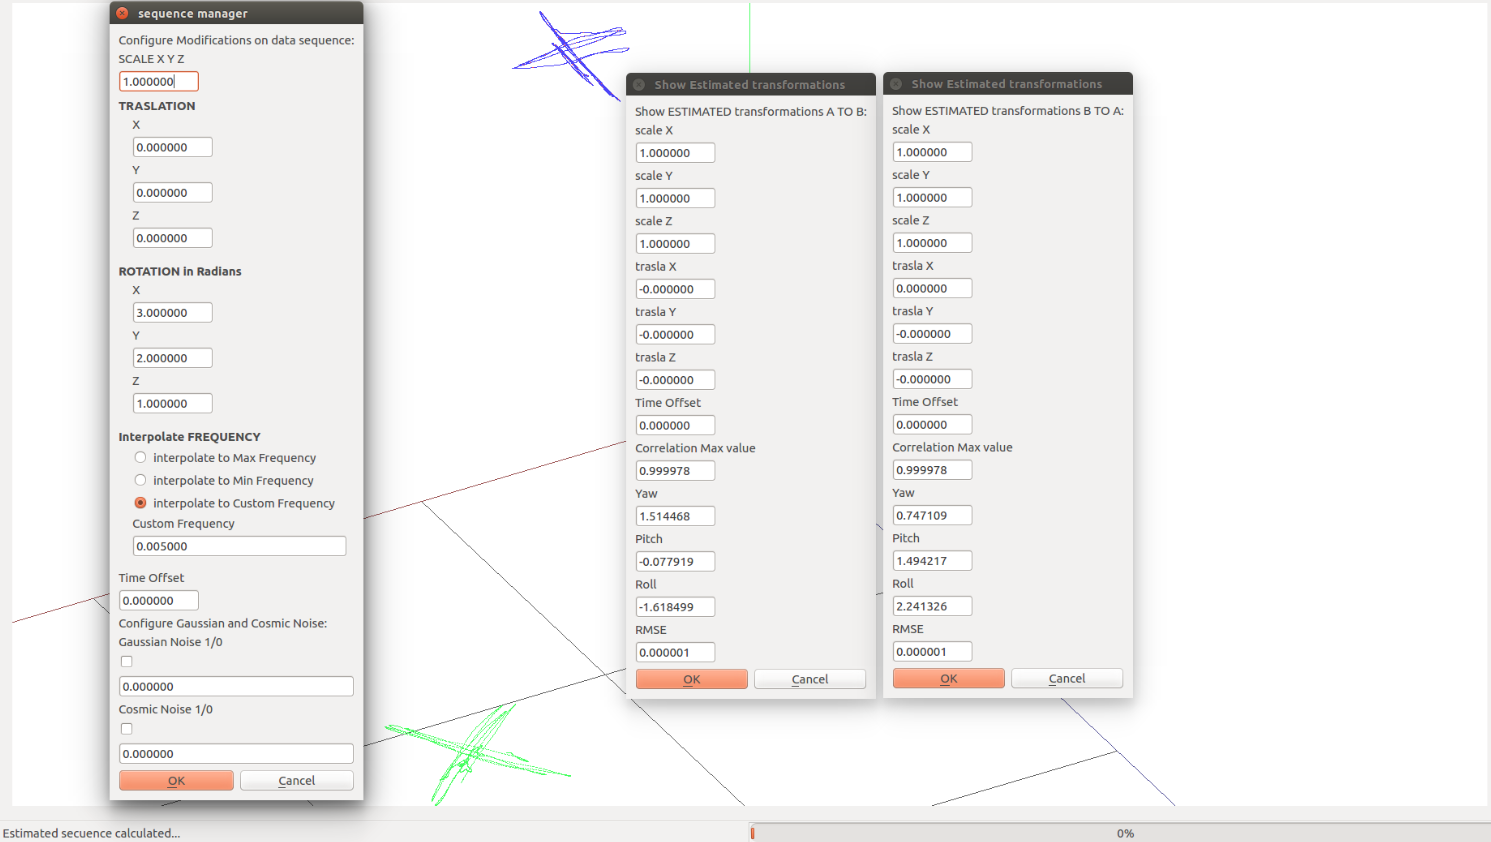
\includegraphics[height=10.0cm,width=15.0cm]{img/cap6/Rotation_abba.png}}
\hspace{0.5cm}

\end{center}

\caption{Gráfico que muestra los resultados de la estimación de un cambio de rotación.}
\end{figure}

En la captura de pantalla anterior, podremos observar el dataset original en verde, y el dataset transformado tras aplicar una rotación. La rotación se especifica en radianes. Como puede observarse, el error (RMSE) es mínimo 0.00001. Se puede comprobar que aunque la rotación realizada en los ejes X,Y,Z en la transformación ha sido respectivamente de 3.0, 2.0 y 1.0 radianes, en la estimación estos valores no coinciden, se ha aplicado otra rotación equivalente en radianes.



\section{Pruebas de transformaciones en parejas}

\begin{figure}[H]
\begin{center}
\subfigure[]{\label{fig:opciones de View}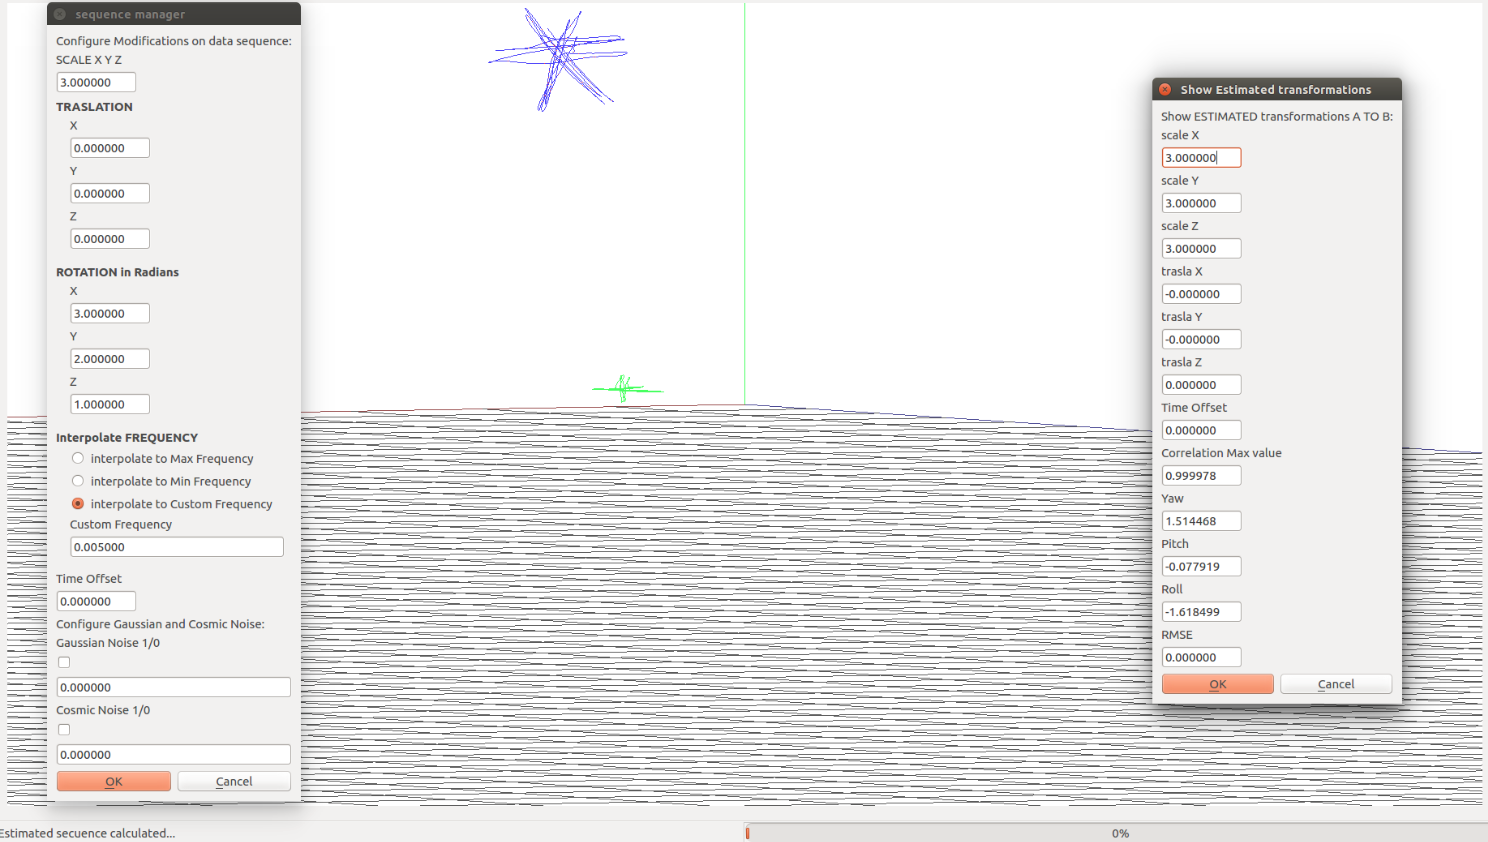
\includegraphics[height=10.0cm,width=15.0cm]{img/cap6/Escala_Traslacion.png}}
\hspace{0.5cm}

\end{center}

\caption{Gráfico que muestra los resultados de la estimación de un cambio de escala y traslación .}
\end{figure}

En la imagen superior, se muestra en color verde, el dataset groundtruth, y en azul el mismo dataset tras realizarle un par de transformaciones en escala y traslación.
En la ventana de la derecha se muestran los resultados de la transformación estimada, que coincide con la transformación realizada, además el RMSE es 0.
El dataset estimado , también se pinta en color rojo, pero en este caso la estimación es tan buena que coincide con el dataset transformado y no se aprecia ningún punto rojo.
En este caso la transformación realizada es de escala y traslación. Se puede comprobar que la estimación realizada es correcta ya que coinciden los valores de la escala y traslación estimados.



\begin{figure}[H]
\begin{center}
\subfigure[]{\label{fig:opciones de View}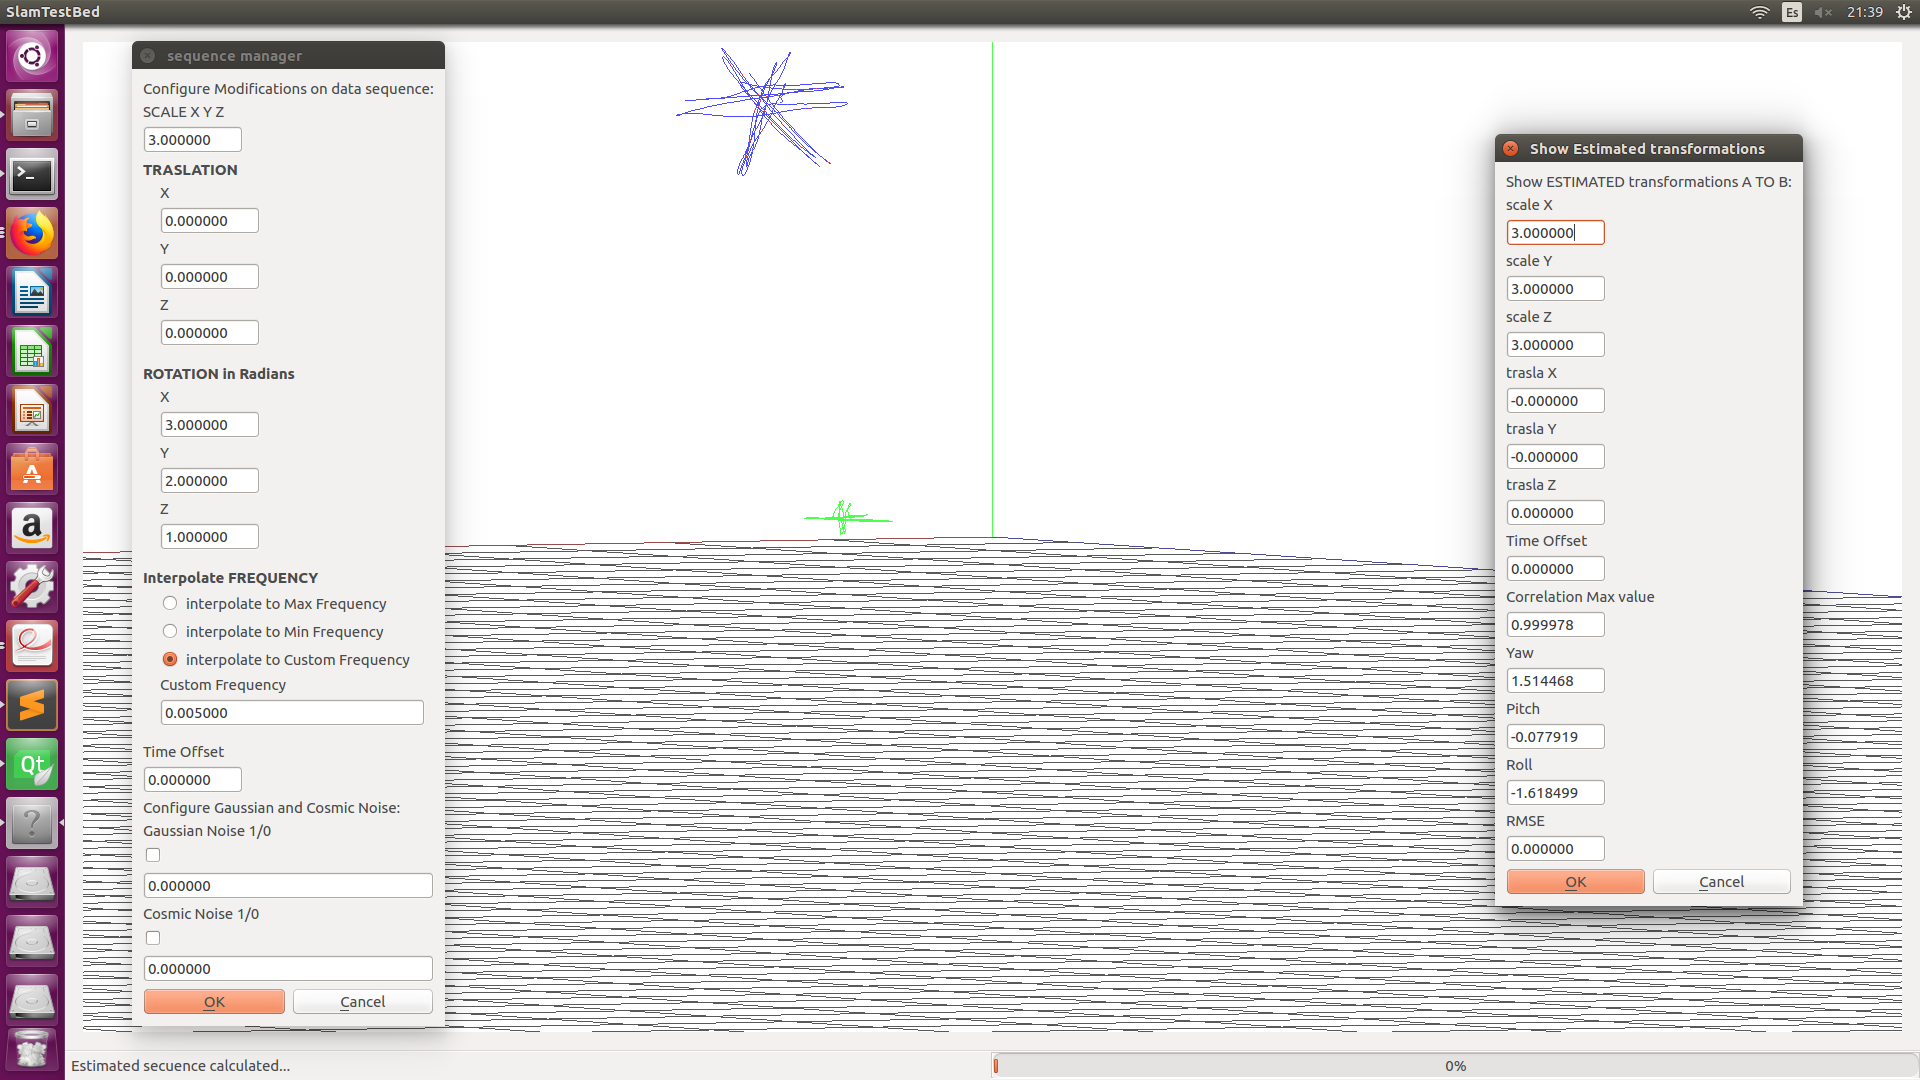
\includegraphics[height=10.0cm,width=15.0cm]{img/cap6/Escala_Rotation.png}}
\hspace{0.5cm}

\end{center}

\caption{Gráfico que muestra los resultados de la estimación de un cambio de escala y rotación.}
\end{figure}
En la imagen superior podemos ver los resultados de aplicar otras 2 transformaciones sobre el dataset original. En este caso se trata de una transformación en escala y rotación.
Tras realizar la estimación, el error medido entre el dataset estimado y el dataset transformado es 0.0 . Por tanto podemos decir que la estimación es exacta a la transformación realizada sobre el dataset original.

\begin{figure}[H]
\begin{center}
\subfigure[]{\label{fig:opciones de View}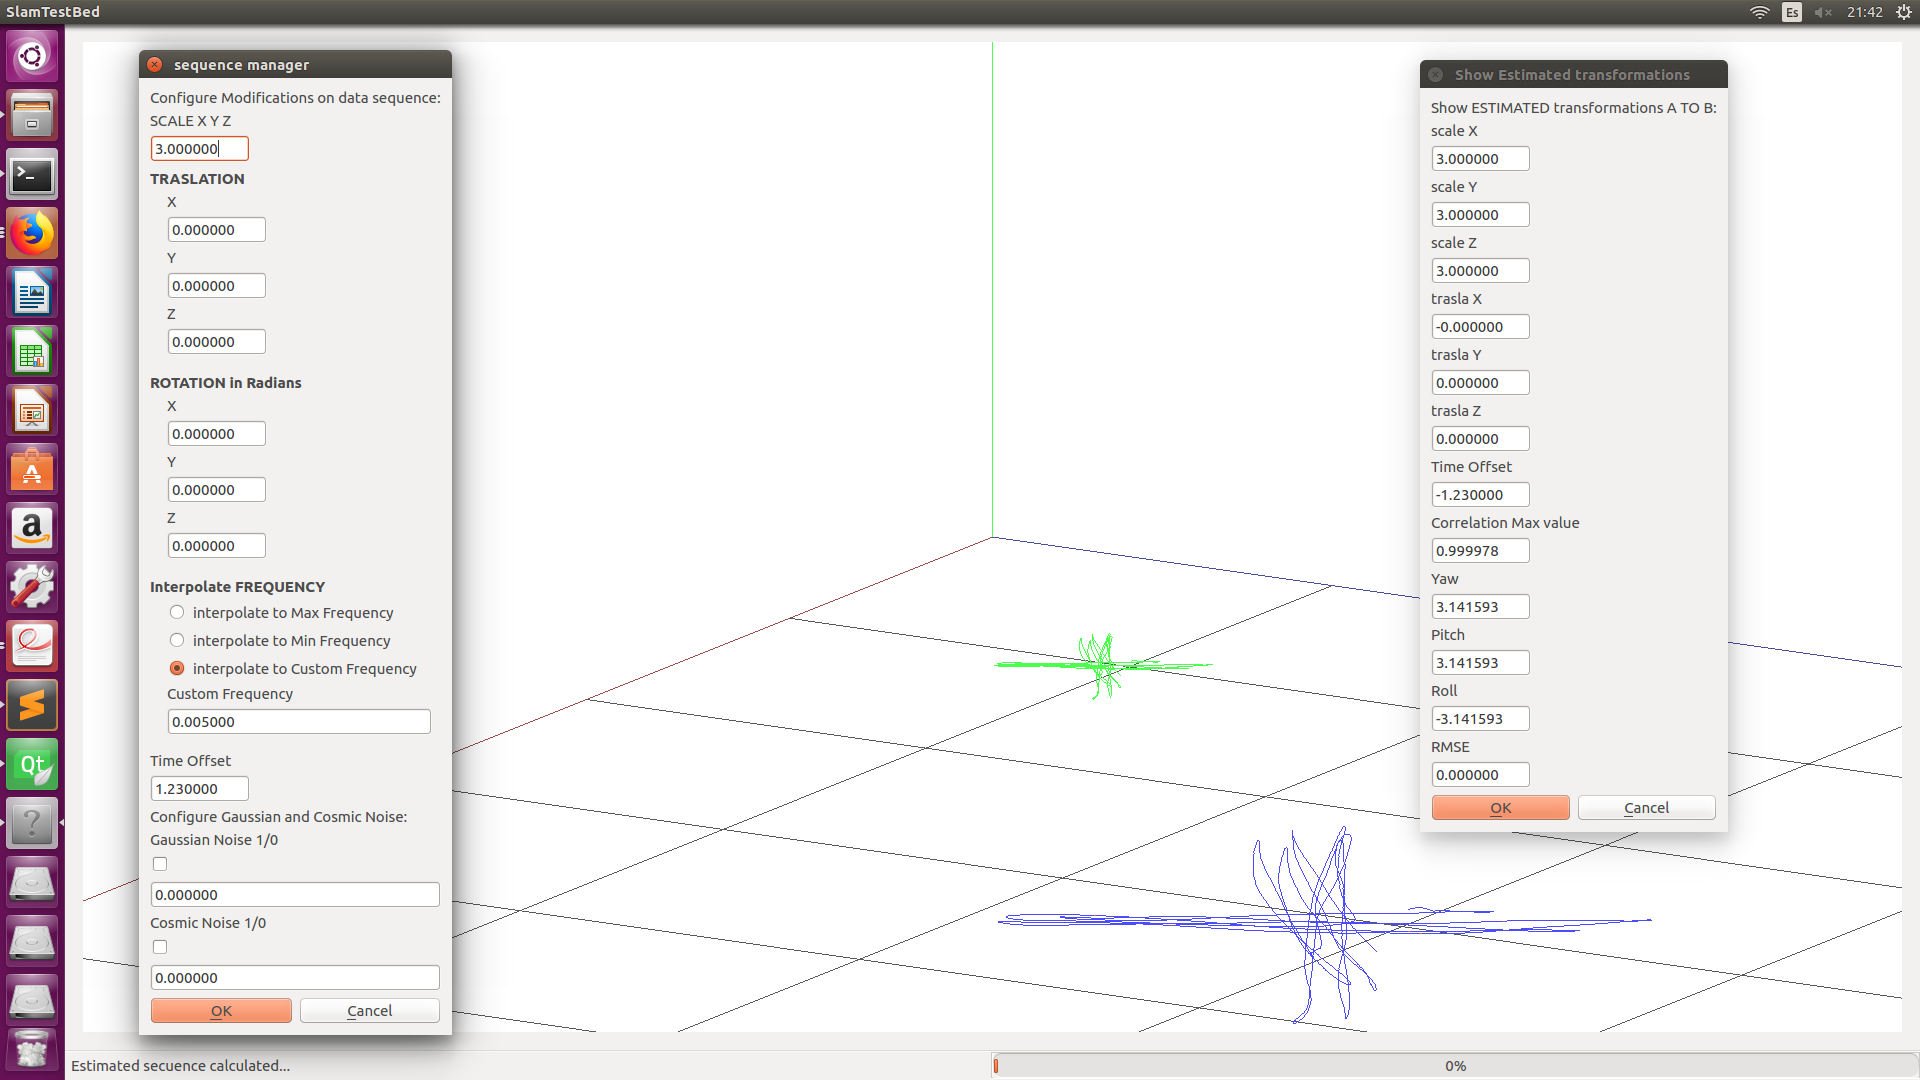
\includegraphics[height=10.0cm,width=15.0cm]{img/cap6/Escala_Offset.png}}
\hspace{0.5cm}

\end{center}

\caption{Gráfico que muestra los resultados de la estimación de un cambio de escala y offset.}
\end{figure}

En este caso, al dataset original (color verde) se le ha aplicado un par de transformaciones ( en escala y con offset), dando lugar al conjunto azul. En este caso tambien la estimación es buena , ya que el error RMSE da como resultado 0.0 y el cálculo del offset tambien coincide con el valor del offset que se ha aplicado en la transformación, salvo con signo negativo.


\begin{figure}[H]
\begin{center}
\subfigure[]{\label{fig:opciones de View}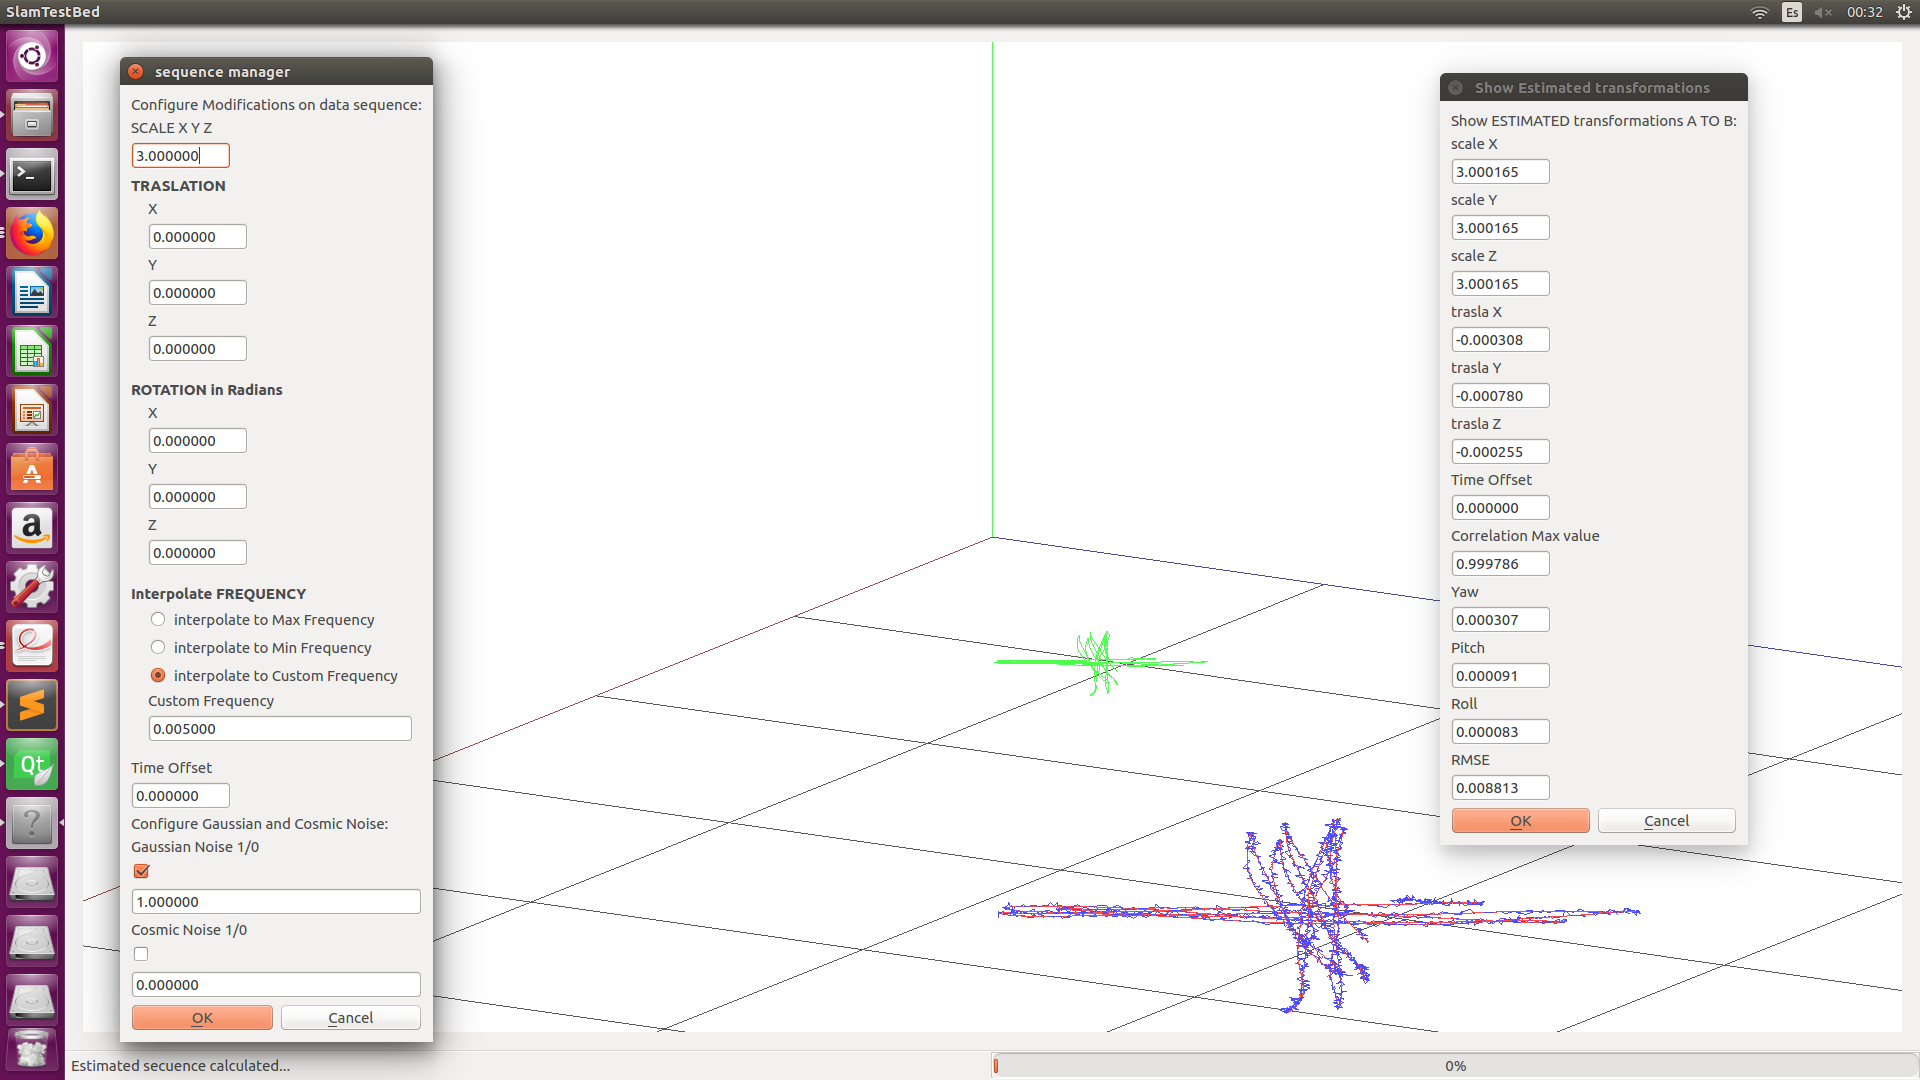
\includegraphics[height=10.0cm,width=15.0cm]{img/cap6/Escala_GaussNoise.png}}
\hspace{0.5cm}

\end{center}

\caption{Gráfico que muestra los resultados de la estimación de un cambio de escala y ruido Gaussiano .}
\end{figure}

En la imagen superior, se ha aplicado sobre el dataset original un cambio de escala y además se le ha añadido ruido Gaussiano, como puede verse en el dataset resultante (color azul). Las estimaciones obtenidas son buenas, pero el error RMSE calculado entre el dataset transformado y el dataset estimando ya no es 0.0, sino 0.008. Esta falta de precisión puede apreciarse a simple vista, ya que como el dataset estimado carece de ruido gaussiano, los puntos del dataset estimado no coinciden con los puntos del dataset transformado, y por tanto ahora si podemos ver buena parte de los puntos del dataset estimado (colo rojo).

\begin{figure}[H]
\begin{center}
\subfigure[]{\label{fig:opciones de View}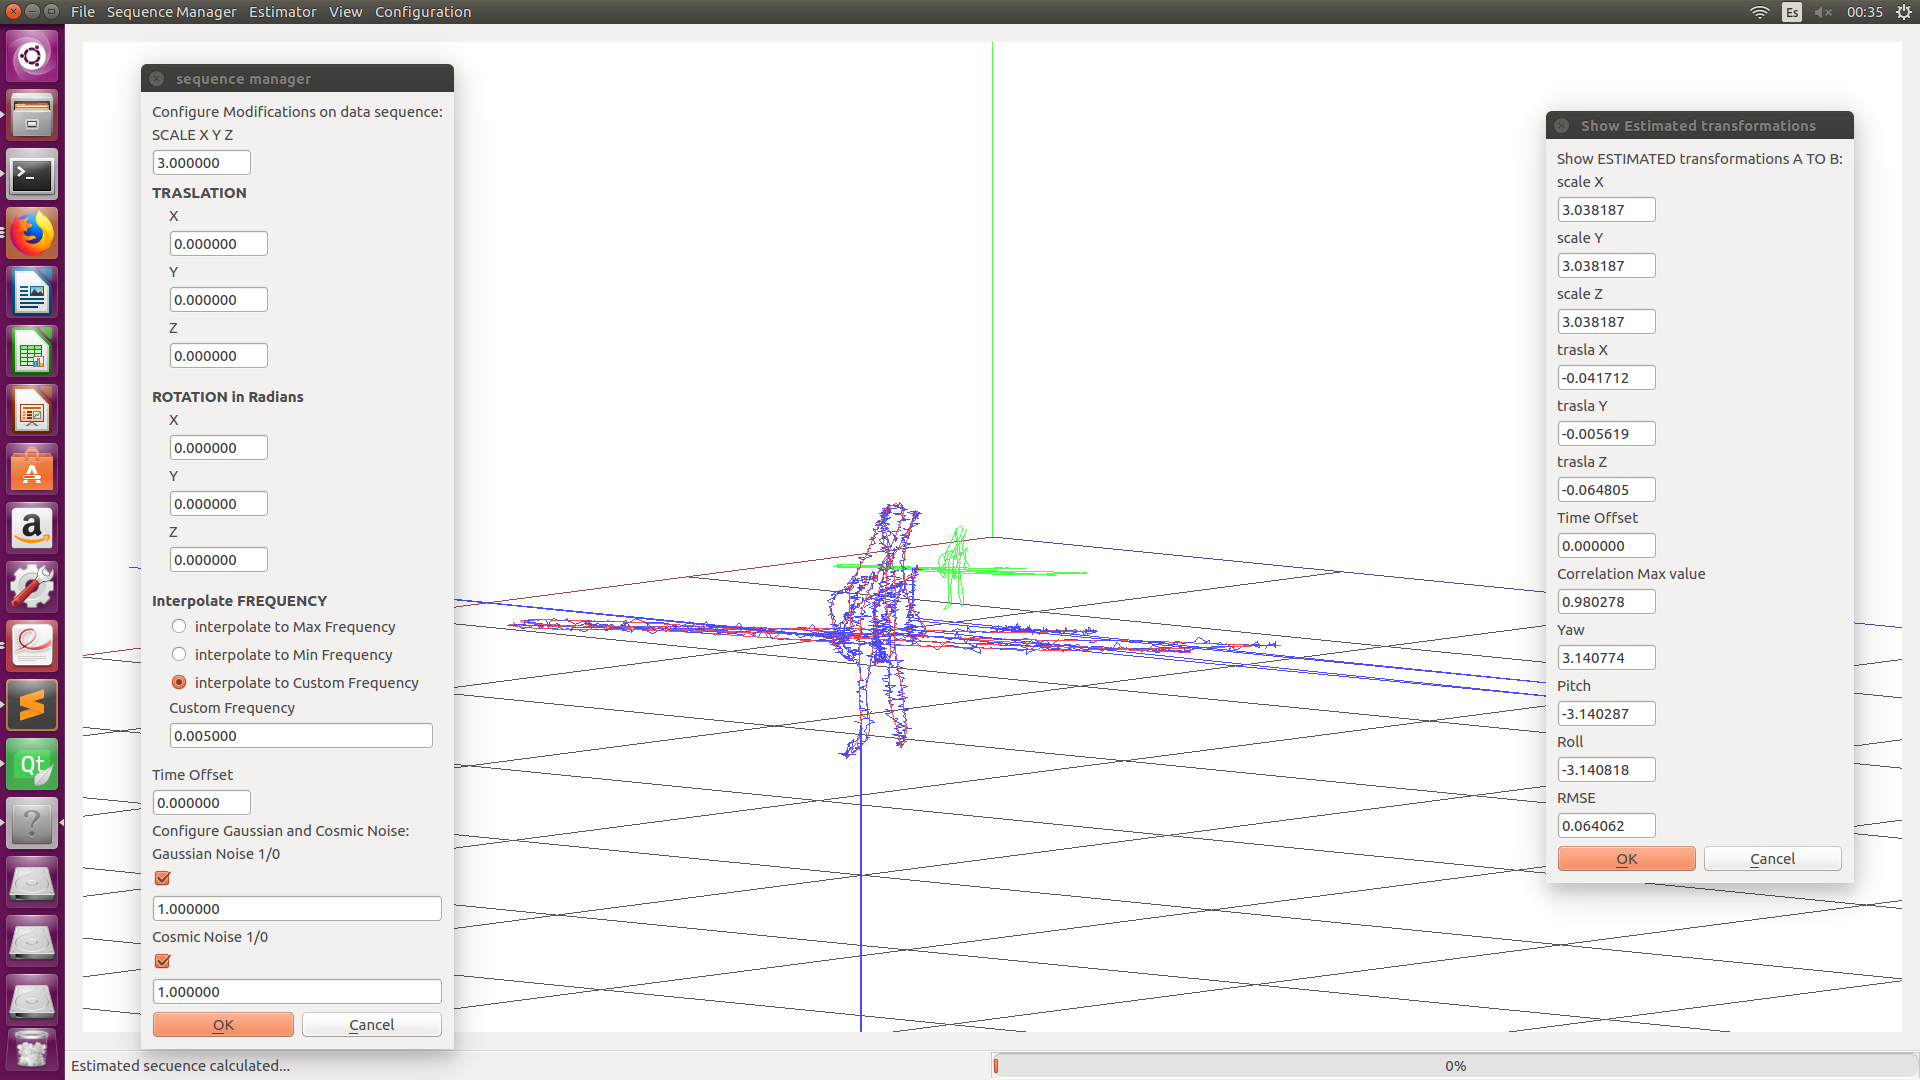
\includegraphics[height=10.0cm,width=15.0cm]{img/cap6/Escala_GaussCosmicNoise.png}}
\hspace{0.5cm}

\end{center}

\caption{Gráfico que muestra los resultados de la estimación de un cambio de escala y traslación .}
\end{figure}

En este caso, se ha aplicado sobre el dataset original un cambio de escala más ruido gaussiano y cósmico. Al tener ahora ruido cósmico, en algunos puntos del dataset transformado aparecen unos valores muy superiores a la media, estos valores desorbitados harán que aumente notablemente el error entre el dataset transformado y el dataset estimado. Para esta experimento , el valor RMSE es de 0.06. Aunque puede observarse que aún así, la posición de los puntos del dataset estimado coincide con la posición de los puntos del dataset transformado.

\begin{figure}[H]
\begin{center}
\subfigure[]{\label{fig:opciones de View}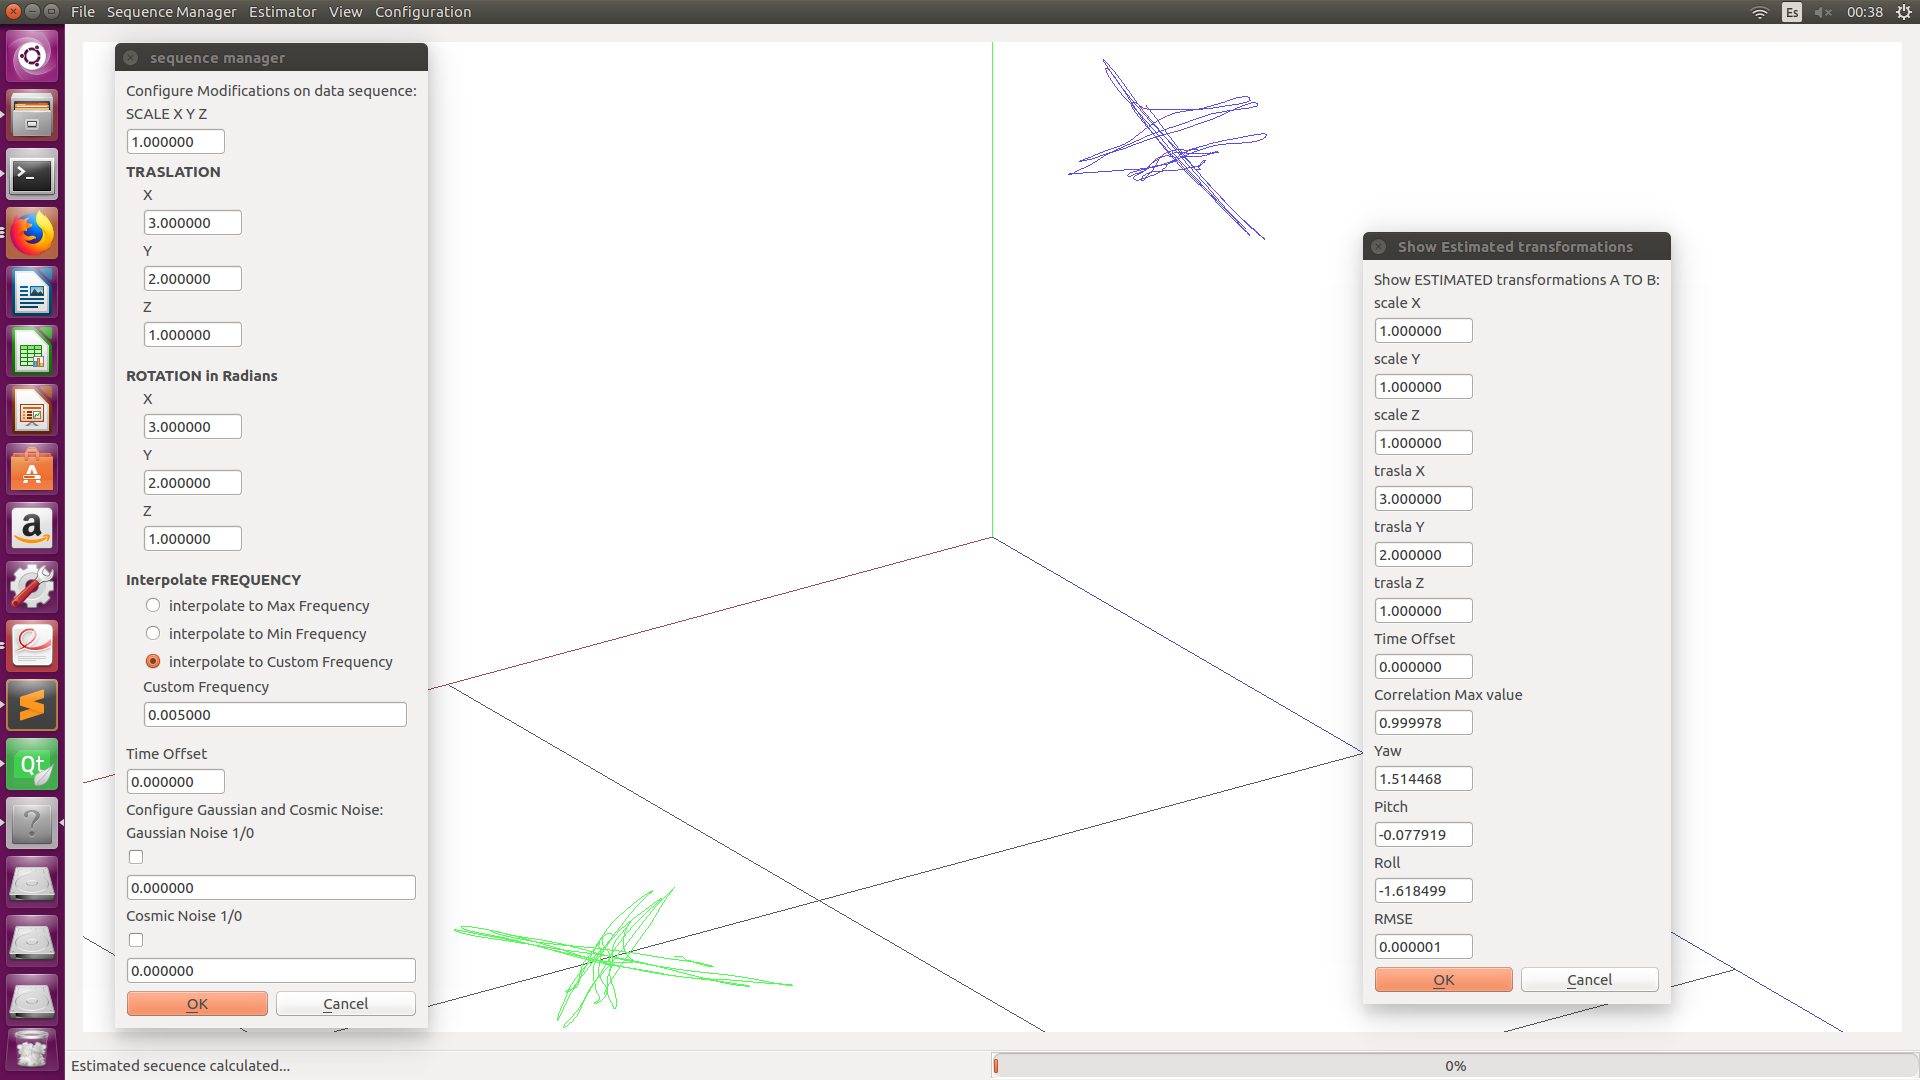
\includegraphics[height=10.0cm,width=15.0cm]{img/cap6/Trasla_Rota.png}}
\hspace{0.5cm}

\end{center}

\caption{Gráfico que muestra los resultados de la estimación de un cambio de traslación y rotación .}
\end{figure}

En este test, se han aplicado 2 transformaciones sobre el dataset original, una traslación y una rotación.
La estimación de la traslación y la rotación coinciden con los valores de las transformaciones. El error calculado entre el dataset estimado y el dataset transformado es 0.000001.
Podríamos considerarlo como 0.0


\begin{figure}[H]
\begin{center}
\subfigure[]{\label{fig:opciones de View}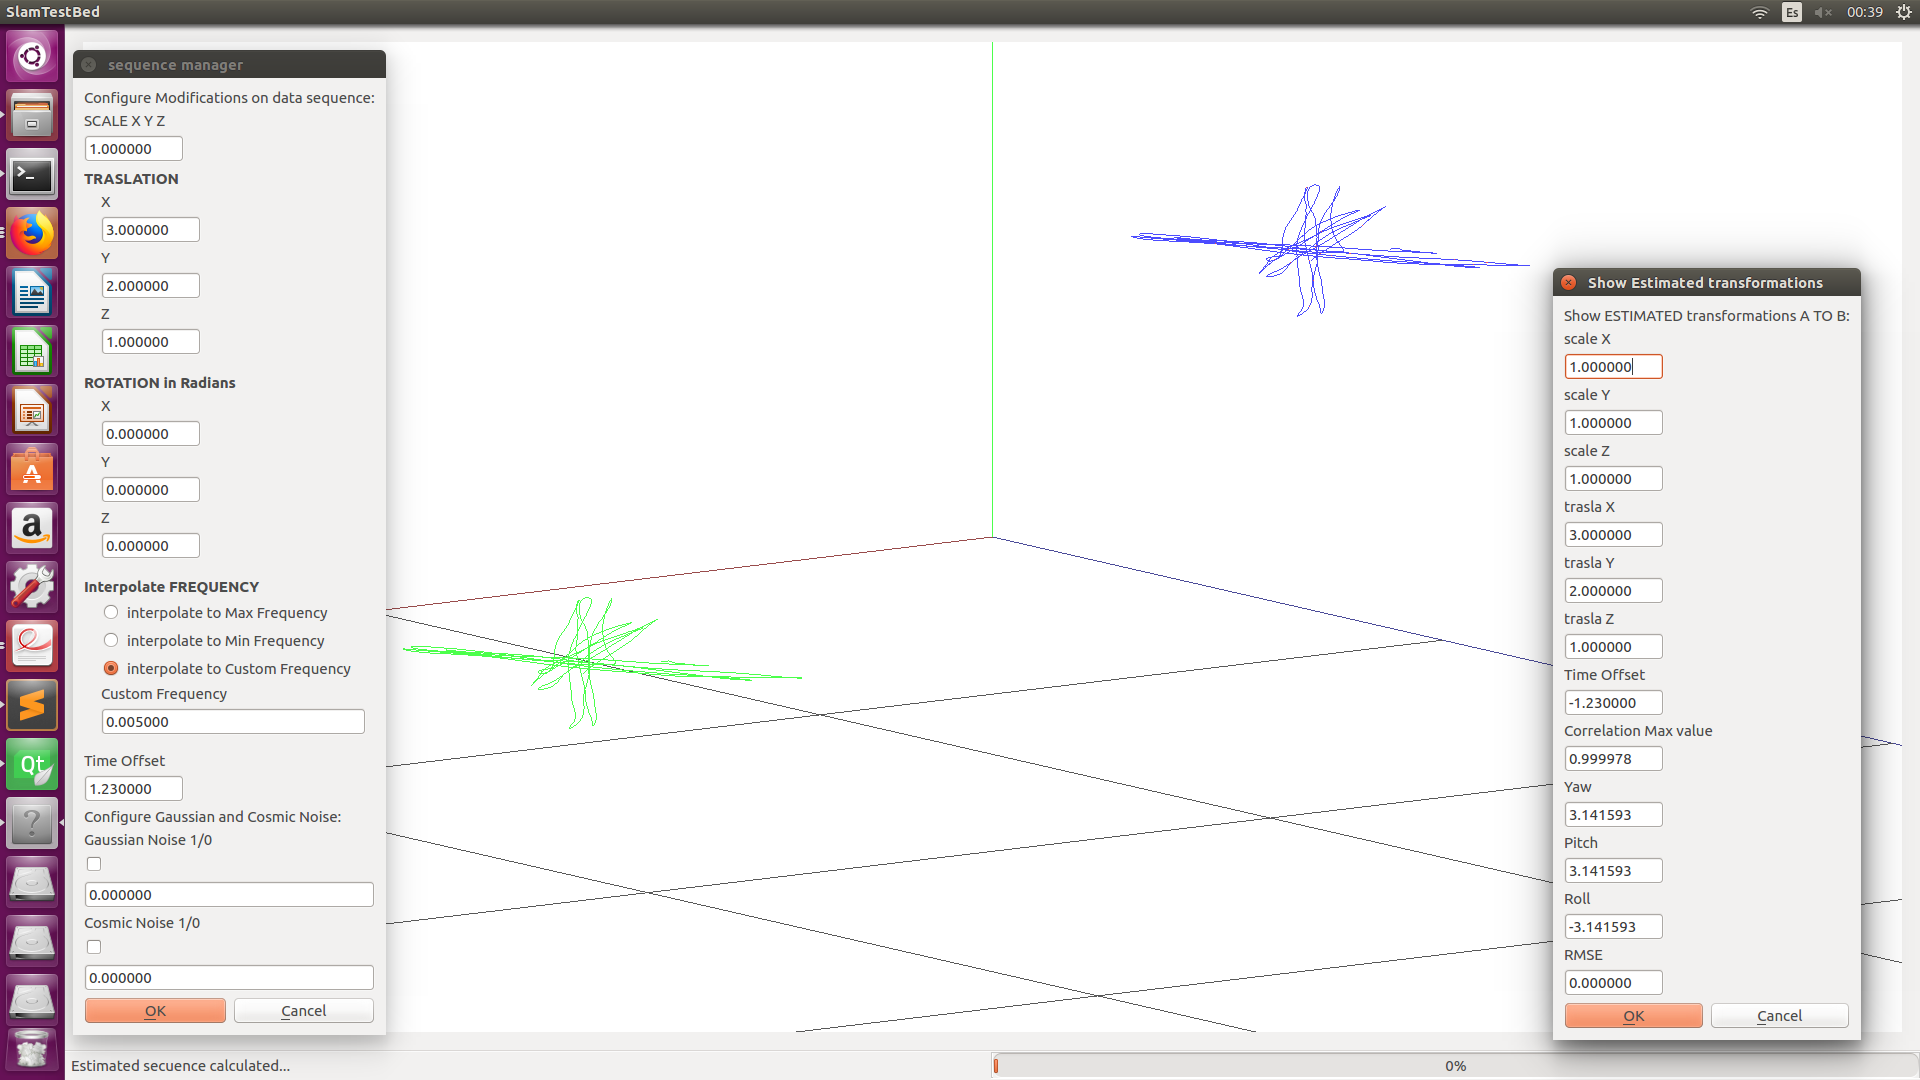
\includegraphics[height=10.0cm,width=15.0cm]{img/cap6/Trasla_Offset.png}}
\hspace{0.5cm}

\end{center}

\caption{Gráfico que muestra los resultados de la estimación de un cambio de traslación y offset .}
\end{figure}
En este caso, al dataset original (color verde) se le ha aplicado un par de transformaciones ( en traslación y con offset), dando lugar al dataset transformado (conjunto de puntos de color azul). En este caso tambien la estimación es buena , ya que el error RMSE da como resultado 0.0 y el cálculo del offset tambien coincide con el valor del offset que se ha aplicado en la transformación, salvo con signo negativo.


\begin{figure}[H]
\begin{center}
\subfigure[]{\label{fig:opciones de View}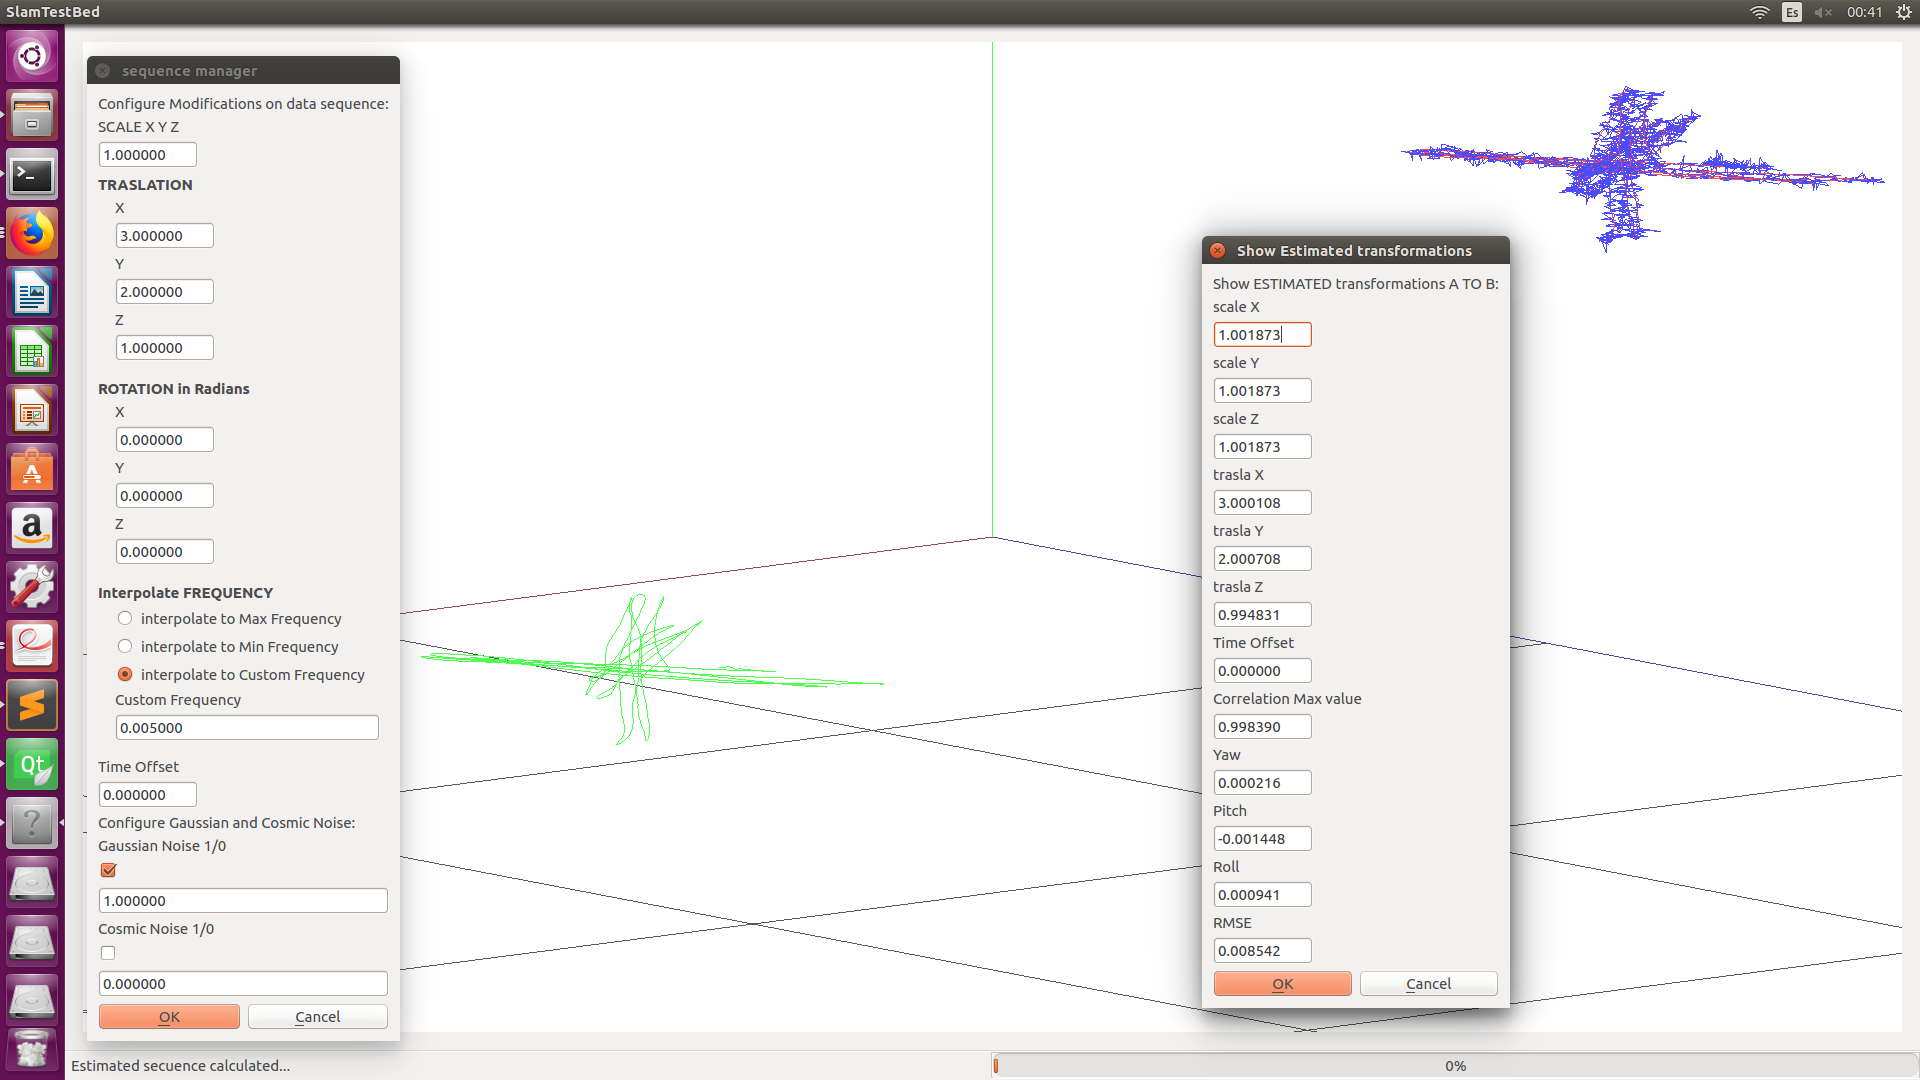
\includegraphics[height=10.0cm,width=15.0cm]{img/cap6/Trasla_GaussNoise.png}}
\hspace{0.5cm}

\end{center}

\caption{Gráfico que muestra los resultados de la estimación de un cambio de traslación y ruido gaussiano.}
\end{figure}
En la imagen superior, se ha aplicado sobre el dataset original un cambio de traslación y además se le ha añadido ruido Gaussiano, como puede verse en el dataset resultante (color azul). Las estimaciones obtenidas son buenas, pero el error RMSE calculado entre el dataset transformado y el dataset estimando ya no es 0.0, sino 0.008. Esta falta de precisión puede apreciarse a simple vista en el interfaz gráfico, ya que como el dataset estimado carece de ruido gaussiano , los puntos del dataset estimado no coinciden con los puntos del dataset transformado, y por tanto ahora si podemos ver buena parte de los puntos del dataset estimado (colo rojo).


\begin{figure}[H]
\begin{center}
\subfigure[]{\label{fig:opciones de View}\includegraphics[height=10.0cm,width=15.0cm]{img/cap6/Trasla_GaussianCosmicNoise.png}}
\hspace{0.5cm}

\end{center}

\caption{Gráfico que muestra los resultados de la estimación de un cambio de traslación y ruido cósmico y gaussiano.}
\end{figure}
En este caso, se ha aplicado sobre el dataset original un cambio de traslación más ruido gaussiano y cósmico. Al tener ahora ruido cósmico, en algunos puntos del dataset transformado aparecen unos valores muy superiores al rango de valores del dataset , estos valores desorbitados harán que aumente notablemente el error entre el dataset transformado y el dataset estimado. Para esta experimento , el valor RMSE es de 0.12. Aunque puede observarse que aún así, la posición de los puntos del dataset estimado coincide con la posición de los puntos del dataset transformado.



\begin{figure}[H]
\begin{center}
\subfigure[]{\label{fig:opciones de View}\includegraphics[height=10.0cm,width=15.0cm]{img/cap6/Rota_Offset.png}}
\hspace{0.5cm}

\end{center}

\caption{Gráfico que muestra los resultados de la estimación de un cambio de rotación y offset.}
\end{figure}

En este caso, al dataset original (color verde) se le ha aplicado un par de transformaciones ( en rotación y con offset tenmporal), dando lugar al dataset transformado (conjunto de puntos de color azul). En este caso tambien la estimación es buena , ya que el error RMSE da como resultado 0.0 y el cálculo del offset tambien coincide con el valor del offset que se ha aplicado en la transformación, salvo con signo negativo.



\begin{figure}[H]
\begin{center}
\subfigure[]{\label{fig:opciones de View}\includegraphics[height=10.0cm,width=15.0cm]{img/cap6/Rota_GaussNoise.png}}
\hspace{0.5cm}

\end{center}

\caption{Gráfico que muestra los resultados de la estimación de un cambio de rotación y ruido gaussiano.}
\end{figure}
En la imagen superior, se ha aplicado sobre el dataset original un cambio de rotación y además se le ha añadido ruido Gaussiano, como puede verse en el dataset resultante (color azul). Las estimaciones obtenidas son buenas, pero el error RMSE calculado entre el dataset transformado y el dataset estimado ya no es 0.0, sino 0.008. Esta falta de precisión puede apreciarse a simple vista en el interfaz gráfico, ya que como el dataset estimado carece de ruido gaussiano , los puntos del dataset estimado no coinciden con los puntos del dataset transformado, y por tanto ahora si podemos ver buena parte de los puntos del dataset estimado (colo rojo).




\begin{figure}[H]
\begin{center}
\subfigure[]{\label{fig:opciones de View}\includegraphics[height=10.0cm,width=15.0cm]{img/cap6/Rota_Gauss_Cosmic.png}}
\hspace{0.5cm}

\end{center}

\caption{Gráfico que muestra los resultados de la estimación de un cambio de rotación y ruido cósmico y gaussiano.}
\end{figure}

En este caso, se ha aplicado sobre el dataset original un cambio de rotación más ruido gaussiano y cósmico. Al tener ahora ruido cósmico, en algunos puntos del dataset transformado aparecen unos valores muy superiores al rango de valores del dataset , estos valores desorbitados harán que aumente notablemente el error entre el dataset transformado y el dataset estimado. Para esta experimento, el valor RMSE es de 0.12. Aunque puede observarse que aún así, la posición de los puntos del dataset estimado coincide con la posición de los puntos del dataset transformado.




\section{Pruebas de transformaciones combinadas}

En este apartado mostraremos los resultados de las estimaciones tras realizar varias transformaciones combinadas. En todas se utiliza la interpolación de tiempo a 0.005 segundos


\begin{figure}[H]
\begin{center}
\subfigure[]{\label{fig:opciones de View}\includegraphics[height=10.0cm,width=15.0cm]{img/cap6/Escala_Trasla_Rota_abba.png}}
\hspace{0.5cm}

\end{center}

\caption{Gráfico que muestra los resultados de la estimación de un cambio de escala y traslación .}
\end{figure}

En la imagen superior se realiza la estimación de las transformaciones necesarias para pasar del datasetA al datasetB . En este caso se ha aplicado una transformación combinada de Escala, Traslación y Rotación. En verde puede verse el dataset original y en azul el dataset transformado, en rojo se aprecia el dataset estimado.
Se puede ver gráficamente como el dataset estimado se ajusta con gran precisión al dataset transformado (azul).
Por otra parte el RMSE entre el dataset transformado y el dataset estimado es de 0.0
Además las transformaciones se han calculado en los 2 sentidos, desde el dataSet A  al dataSet B y desde el dataSetB al dataSet A.


\begin{figure}[H]
\begin{center}
\subfigure[]{\label{fig:opciones de View}\includegraphics[height=10.0cm,width=15.0cm]{img/cap6/Escala_Trasla_Rota_Offset_abba.png}}
\hspace{0.5cm}

\end{center}

\caption{Gráfico que muestra los resultados de la estimación de un cambio de escala, traslación,rotación y offset .}
\end{figure}

Arriba en la imagen , se presenta el dataset original en verde, el dataset transformado en azul y el dataset estimado en rojo.
En este caso se ha realizado la siguiente combinación de transformaciónes, Escala, Traslación, Rotación y Offset.
Como se puede observar en los resultados de las estimaciones, el offset es estimado con total exactitud. Sin embargo el valor del RMSE ya no es de 0.0, si no de 0.0005, aún así el error cometido sigue siendo muy bajo.
Visualmente, también se puede observar que la precisión ha disminiuido , ya que se aprecian más puntos rojos (dataset estimado) en el gráfico. Esto indica que la estimación sigue siendo muy buena aunque la precisión ha bajado.


\begin{figure}[H]
\begin{center}
\subfigure[]{\label{fig:opciones de View}\includegraphics[height=10.0cm,width=15.0cm]{img/cap6/Escala_Trasla_Rota_Offset_GaussNoise_abba.png}}
\hspace{0.5cm}

\end{center}

\caption{Gráfico que muestra los resultados de la estimación de un cambio de escala y traslación .}
\end{figure}

En la imagen superior, podemos ver el dataset original en verde, el dataset transformado en azul y el dataset estimado en rojo.
Las transformaciones realizadas en este caso han sido, Escala, Traslación, Rotación, Offset y Ruido Gaussiano.
En este caso, al incluir ruido Gaussiano en la transformación del dataset original, el dataset estimado pierde precisión, y el RMSE obtenido es de  0.008.
Sin embargo, la precisión aunque es menor, continúa siendo buena, y en el gráfico puede verse , como el dataset estimado concuerda de manera aceptable con el dataset estimado.
Observesé que en el dataset estimado no hay ruido gaussiano.


\begin{figure}[H]
\begin{center}
\subfigure[]{\label{fig:opciones de View}\includegraphics[height=10.0cm,width=15.0cm]{img/cap6/Escala_Trasla_Rota_Offset_Gauss_CosmicNoise_abba.png}}
\hspace{0.5cm}

\end{center}

\caption{Gráfico que muestra los resultados de la estimación de un cambio de escala y traslación .}
\end{figure}

Arriba podemos ver una nueva captura de pantalla, donde se han realizado las siguientes transformaciones, Escala, Traslación, Rotación, Offset, Ruido Gaussiano y Ruido Cósmico.
Como se puede observar, en las estimaciones del dataset A ( verde ) al dataset B (azul), la precisión ha bajado notablemente, con un valor RMSE del 0.06.
Esta precisión tan baja se debe a la incluisión de ruido Cósmico, que altera notablemente los valores de X, Y , Z  de algunos puntos 3D.
Aún así, como puede verse en  la representación gráfica del dataset Estimado (rojo) sobre el dataset Transformado ( azul ) se aproxima bastante a la solución óptima.



\begin{figure}[H]
\begin{center}
\subfigure[]{\label{fig:opciones de View}\includegraphics[height=8.0cm,width=12.0cm]{img/cap6/LoadTwoDataSets_RANSAC.png}}
\hspace{0.5cm}

\end{center}

\caption{Gráfico que muestra los resultados de la estimación de la transformación del datasetA en el datasetB y viceversa, utilizando RANSAC.}
\end{figure}

En captura de pantalla superior, podremos ver una nueva transformación donde se ha aplicado transformaciónes de Escala, Traslación, Rotación, Offset, Ruido Gaussiano y Cósmico y además se ha utilizado el método RANSAC para calcular el error.

\clearpage





%\begin{figure}[H]
%\begin{center}
%\subfigure[]{\label{fig:opciones de View}\includegraphics[height=8.0cm,width=12.0cm]{img/cap6/ScaleTraslaFrec.png}}
%\hspace{0.5cm}

%\end{center}

%\caption{Gráfico que muestra los resultados de la estimación de un cambio de escala, traslación y frecuencia.}
%\end{figure}


%\begin{figure}[H]
%\begin{center}
%\subfigure[]{\label{fig:opciones de View}\includegraphics[height=8.0cm,width=12.0cm]{img/cap6/ScaleTraslaRotaFrec.png}}
%\hspace{0.5cm}

%\end{center}

%\caption{Gráfico que muestra los resultados de la estimación de un cambio de escala, traslación,rotación y frecuencia.}
%\end{figure}


%\begin{figure}[H]
%\begin{center}
%\subfigure[]{\label{fig:opciones de View}\includegraphics[height=8.0cm,width=12.0cm]{img/cap6/ScaleTraslaRotaFrecGNoiseCNoise.png}}
%\hspace{0.5cm}

%\end{center}

%\caption{Gráfico que muestra los resultados de la estimación de un cambio de escala, traslación, rotación, frecuencia, ruido gaussiano y ruido cósmico.}
%\end{figure}



%\begin{figure}[H]
%\begin{center}
%\subfigure[]{\label{fig:opciones de View}\includegraphics[height=8.0cm,width=12.0cm]{img/cap6/ScaleTraslaRotaFrecTimeOffset.png}}
%\hspace{0.5cm}

%\end{center}

%\caption{Gráfico que muestra los resultados de la estimación de un cambio de escala, traslación, rotación, frecuencia y offset.}
%\end{figure}


%\begin{figure}[H]
%\begin{center}
%\subfigure[]{\label{fig:opciones de View}\includegraphics[height=8.0cm,width=12.0cm]{img/cap6/ScaleTraslaRotaFrecTimeOffset2.png}}
%\hspace{0.5cm}

%\end{center}

%\caption{Gráfico que muestra los resultados de la estimación de un cambio de escala, traslación, rotación, frecuencia y offset.}
%\end{figure}



%\begin{figure}[H]
%\begin{center}
%\subfigure[]{\label{fig:opciones de View}\includegraphics[height=8.0cm,width=12.0cm]{img/cap6/ScaleTraslaRotaFrecTimeOffsetGNoiseCNoise.png}}
%\hspace{0.5cm}

%\end{center}

%\caption{Gráfico que muestra los resultados de la estimación de un cambio de escala, traslación, rotación, frecuencia, Offset, Ruido Gausiano y Ruido Cósmico.}
%\end{figure}




%\begin{figure}[H]
%\begin{center}
%\subfigure[]{\label{fig:opciones de View}\includegraphics[height=8.0cm,width=12.0cm]{img/cap6/TraslaRotaFrecGnoiseCnoise.png}}
%\hspace{0.5cm}

%\end{center}

%\caption{Gráfico que muestra los resultados de la estimación de un cambio de traslación, rotación, frecuencia, Ruido Gaussiano y Ruido Cósmico.}
%\end{figure}


%Por último también mostraremos como SLAMTestBed es capaz de operar con 2 datasets diferentes , es decir en este caso , el seguno dataset no será el resultado de aplicar el módulo %de transformación sobre el primer dataset.

%\begin{figure}[H]
%\begin{center}
%\subfigure[]{\label{fig:opciones de View}\includegraphics[height=8.0cm,width=12.0cm]{img/cap6/LoadTwoDataSets.png}}
%\hspace{0.5cm}

%\end{center}

%\caption{Gráfico que muestra los resultados de la estimación de la transformación del datasetA en el datasetB y viceversa.}
%\end{figure}


%\begin{figure}[H]
%\begin{center}
%\subfigure[]{\label{fig:opciones de View}\includegraphics[height=8.0cm,width=12.0cm]{img/cap6/LoadTwoDataSets_RANSAC.png}}
%\hspace{0.5cm}

%\end{center}

%\caption{Gráfico que muestra los resultados de la estimación de la transformación del datasetA en el datasetB y viceversa, utilizando RANSAC.}
%\end{figure}

%\clearpage


 %5
\newpage
\newpage

\chapter{Conclusiones} \label{cap:conclusiones}
%\section{Conclusiones} \label{s:conclusiones}

Se ha diseñado y programado una aplicación, llamada SLAMTestbed, que estima las relaciones entre dos secuencias de puntos 3D orientados, calculando tanto sus relaciones espaciales ( qué traslación, rotación y escala hay entre ellas) como sus relaciones temporales (qué desfase temporal existe ellas).

Esto lo consigue incluso con dos secuencias de puntos 3D que no están expresadas en el mismo sistema de referencia espacial, ni con la misma escala, ni con la misma frecuencia de muestras, ni con el mismo origen de tiempos. Para ello, incluye varios bloques específicos de estimación encadenando diferentes estimadores, análisis matemáticos y módulos de registro.

Esta aplicación permite medir objetiva y cuantitativamente el error en las estimaciones de un algoritmo de Visual SLAM cuando se introducen sus estimaciones y la secuencia de posiciones verdaderas en la herramienta SLAMTestbed. En ese caso las diferencias entre ambas secuencias y los estadísticos calculados reflejan la calidad y la exactitud de las estimaciones del algoritmo.
Además de caracterizar sus calidad objetivamente permite por tanto compararlo con otros algoritmos de Visual SLAM o diferentes variantes del mismo algoritmo.


\section{Conclusiones}

El objetivo principal de este proyecto es ofrecer una herramienta software que permita medir cuantitativamente el rendimiento de los algoritmos Visual SLAM y la calidad de sus estimaciones.
Este objetivo se ha logrado con el diseño e implementación de un Registrador Temporal (subobjetivo 1) y otro Registrador Espacial (subobjetivo 2). 
Para crear el Registrador Temporal ha sido necesario desarrollar un módulo que calcule el desplazamiento de tiempo entre dos secuencias (capítulo 4.3) y tambien un módulo interpolador (capítulo 4.4) capaz de sincronizar en frecuencia los dos \textit{datasets} de entrada. Para validar el correcto funcionamiento de los Registradores Temporal y Espacial, se ha creado un módulo Transformador (subobjetivo 3) tal y como se ha comentado en el capítulo 5.1.
Para validar experimentalmente estos dos módulos de registro se han hecho múltiples pruebas de distinta complejidad como se describe en el capítulo 5.2, 5.3 y 5.4.

La herramienta SLAMTestbed incorpora además un interfaz gráfico que permite al usuario visualizar en 3D las secuencias de datos así como lanzar operaciones sobre los datasets de una forma tan sencilla como hacer click con el ratón y mostrar los resultados por pantalla (capítulo 4.7). Se debe tener en cuenta que no todas las herramientas de algoritmos SLAM que existen actualmente incorporan este interfaz gráfico, como por ejemplo TUM (capítulo 3.2), que a día de hoy sólo permite lanzar comandos desde un terminal. Esto es una ventaja para SLAMTestbed, ya que, como se ha demostrado en las pruebas, este interfaz es útil para verificar con un simple vistazo si la estimación es correcta o por el contraio se aleja de la verdad absoluta.

En cuanto a las pruebas de validación de la herramienta, hemos comprobado que estima con gran exactitud las transformaciones entre datasets. Pero se ha demostrado que la precisión de las estimaciones se degrada de manera considerable ante la presencia de ruido cósmico, ya que genera datos espúreos en los datasets. Para suavizar la presencia de espúreos se ha verificado que la utilización de algoritmos RANSAC mejora los resultados de las estimaciones.


\section{Líneas Futuras}

En este subapartado describiremos en que líneas se debería trabajar o profundizar más en el futuro en la herramienta SLAMTestbed:

\begin{enumerate}

\item{Uso de SLAMTestbed para comparar diferentes algoritmos del estado del arte de Visual SLAM utilizando datasets internacionales de referencia que incluyan verdad absoluta.}

\item{Utilización de SLAMTestbed en el TFM de Javier Martinez para medir si la introducción de sensor inercial mejora o no la calidad de las estimaciones de posición en el algoritmo SD-slam.}

\item{Incorporar más estadísticas y medidas de error que ayuden a evaluar la precisión y robustez del algoritmo, como por ejemplo el porcentaje de tiempo en que la diferencia entre trayectorias es menor que un umbral.}

\item{Escritura de un artículo científico que presente esta herramienta a la comunidad investigadora.}

\item{Nuevas opciones y mejoras en el interfaz de usuario para modificar parámetros como la distribución del ruido gaussiano, valores límite para el ruido cósmico, o utilización de varios hilos de proceso para que el interfaz no se quede bloqueado mientras realiza cálculos.}

\item{Añadir nuevos algoritmos en el módulo de Registro, como Horn, Horn + RANSAC y posibilidad de que la herramienta seleccione automáticamente el algoritmo de registro que 
mejores resultados obtenga.}

\item{Portabilidad de la herramienta a otros lenguajes de programación (python,Java) o sistemas operativos (Android).}

\end{enumerate}

Todo el código de la herramienta SLAMTestbed está publicado en el repositorio GitHub, lo cual abre su desarrollo y mantenimiento a la comunidad de usuarios e investigadores que quieran utilizar esta herramienta.


 %6
\endgroup

\nocite{*}

\bibliographystyle{named}
\bibliography{bibliografia}

\end{document}
